\documentclass[11pt,a4paper]{article}

% ─── Packages ────────────────────────────────────────────────────────────────
\usepackage[utf8]{inputenc}
\usepackage[T1]{fontenc}
\usepackage{lmodern}
\usepackage{microtype}
\usepackage{geometry}
\usepackage{amsmath,amssymb,amsthm}
\usepackage{listings}
\usepackage{xcolor}
\usepackage{booktabs}
\usepackage{tabularx}
\usepackage{array}
\usepackage{graphicx}
\usepackage{fancyhdr}
\usepackage{tikz}
\usepackage{pgfplots}
\pgfplotsset{compat=1.18}
\usetikzlibrary{arrows.meta,positioning,fit,backgrounds,calc,shapes.geometric,shapes.symbols,decorations.pathmorphing,decorations.pathreplacing}
\usepackage{float}
\usepackage{caption}
\usepackage{enumitem}
\usepackage[backref=page]{hyperref}
\captionsetup{font=small,labelfont=bf}

\geometry{margin=2.5cm}

\newif\ifpdswiss\pdswisstrue
\newif\ifpdmaritime
\newif\ifpdtechnical

\definecolor{codebg}{RGB}{248,248,248}
\definecolor{codeframe}{RGB}{200,200,200}
\definecolor{hhsand}{HTML}{E9DCC4}
\definecolor{hhsanddeep}{HTML}{D8C7A6}
\definecolor{hhebony}{HTML}{121212}
\definecolor{hhink}{HTML}{1B1712}
\definecolor{hhcobalt}{HTML}{003FB8}
\definecolor{hhamber}{HTML}{6B4500}
\definecolor{hhteal}{HTML}{00564C}
\definecolor{hhpaper}{HTML}{FBF7EF}
\definecolor{hhgray}{HTML}{5C5650}
% The Book's semantic color system: palette v2, light values. One hue, one meaning.
% Source of record for every hex: website-v2/src/styles/tokens.semantic.css (light
% theme); website-v2/scripts/check-figure-palette.mjs fails the build if this file
% and the tokens disagree. Twin copy under whitepaper/figures/ (byte-identical).
%
% Discipline: story colors are accents (rules, fills, marks, display text); body
% pages stay cream and ink. Amber is stripes, dots, and display only, never small
% text (3.71:1 on cream). Violet and gold are AA as text; use them at display size
% or on rules and fills. Line weights: 1px texture, 1.5px linework, 2px enclosure.
\definecolor{pdcobalt}{HTML}{003FB8}      % kernel / truth            --brand-primary
\definecolor{pdteal}{HTML}{006B5F}        % legibility                --brand-accent
\definecolor{pdhealth}{HTML}{1F7A4D}      % ready / coordinated       --story-health
\definecolor{pdindigo}{HTML}{353A85}      % protocol / federation     --story-indigo
\definecolor{pdviolet}{HTML}{933FA5}      % identity / continuity     --story-violet
\definecolor{pdrust}{HTML}{7A4514}        % reputation / trust earned --story-rust
\definecolor{pdgold}{HTML}{666A00}        % economy / value           --story-gold
\definecolor{pdslate}{HTML}{384856}       % foundation / bedrock      --story-slate
\definecolor{pderror}{HTML}{BF2F2F}       % breach / correction       --status-error
\definecolor{pdamber}{HTML}{A66F00}       % warning (display only)    --status-warning
\definecolor{pdlime}{HTML}{CAD900}        % highlight fill, ink text  --chart-yellow
\definecolor{pdink}{HTML}{121212}         % ink                       --text-primary
\definecolor{pdinkmuted}{HTML}{403B34}    % links, secondary text     --text-secondary
\definecolor{pdcream}{HTML}{F2EEE6}       % page ground               --surface-base
\definecolor{pdcreamraised}{HTML}{F7F3EB} % panels                    --surface-raised
\definecolor{pdcreamstrong}{HTML}{E9E2D5} % inset wells               --surface-strong
% Print inks for the Swiss edition of the Book (SWISS-BRIEF, B); print only.
\definecolor{pdswissblue}{HTML}{001489}
\definecolor{pdswissviolet}{HTML}{582C83}
\definecolor{pdswissred}{HTML}{DA291C}
% And the maritime edition's fourth ink: antique gold, the trim of the engraved
% plates carried onto the page (opener rules, part-title ornament, fillets round
% framed matter). Flat stand-in for a metallic pass; print only.
\definecolor{pdmaritimegold}{HTML}{805A14}

\newcommand{\pdchapterprefix}{none}% Chapter 0: Prerequisites (prefix none before numbered chapters)
% GENERATED FILE. Do not edit by hand.
% Source of record: whitepaper/textbook.json (chapter order, numbers, parts, edition).
% Regenerate both committed copies: node scripts/generate-mega-whitepaper.mjs --sync-shared
% Drift check (CI): node --test scripts/generate-mega-whitepaper.test.mjs
% Twin copies: whitepaper/figures/pd-textbook-map.tex and
%              website-v2/public/whitepaper/figures/pd-textbook-map.tex (byte-identical).
%
% Every standalone chapter preamble defines \pdchapterprefix before inputting
% this file; the Book redefines it at every \pdchapter. Everything else derives.

\providecommand{\pdeditiontitle}{Governing AI Agents: The Harbor, the Person, and the Economy}
\providecommand{\pdeditionsubtitle}{A Textbook of Concurrency, Identity, and Accountable Autonomous Work}
\providecommand{\pdeditionversion}{4.0 (Textbook Edition)}
\providecommand{\pdeditiondate}{September 2026}
\providecommand{\pdeditionclaim}{For autonomous work to remain accountable, each action needs an authority, a record, and someone responsible for its consequences.}
\providecommand{\pdbooktitle}{\emph{\pdeditiontitle}}
\providecommand{\pdchaptercount}{8}
\providecommand{\pdchaptercountword}{eight}
\providecommand{\pdpartcount}{4}
\providecommand{\pdchapterprefix}{none}
\expandafter\providecommand\csname pdchapternumberofnone\endcsname{0}
\expandafter\providecommand\csname pdchaptertitleofnone\endcsname{\pdeditiontitle}
\expandafter\providecommand\csname pdchaptercolorofnone\endcsname{pdcobalt}
\expandafter\providecommand\csname pdchapternumberofswk\endcsname{1}
\expandafter\providecommand\csname pdchaptertitleofswk\endcsname{The Single-Writer Kernel}
\expandafter\providecommand\csname pdchaptercolorofswk\endcsname{pdcobalt}
\expandafter\providecommand\csname pdchapterformerofswk\endcsname{II}
\expandafter\providecommand\csname pdchapterpartindexofswk\endcsname{1}
\expandafter\providecommand\csname pdchapterpartlabelofswk\endcsname{Part I \textperiodcentered\ Ground Truth}
\expandafter\providecommand\csname pdchapterquestionofswk\endcsname{Where can a rule be made real?}
\expandafter\providecommand\csname pdchapteronelineofswk\endcsname{One writer orders changes to a local database; the chapter specifies which failures that record can survive.}
\expandafter\providecommand\csname pdchapterepigraphofswk\endcsname{There is no fundamental need to keep a database at all; the log is all the information there is. The only reason for storing the database is performance of retrieval operations.}
\expandafter\providecommand\csname pdchapterepigraphsourceofswk\endcsname{Jim Gray and Andreas Reuter, Transaction Processing: Concepts and Techniques, 1993}
\expandafter\providecommand\csname pdchapternumberofanchor\endcsname{2}
\expandafter\providecommand\csname pdchaptertitleofanchor\endcsname{The Anchor Protocol}
\expandafter\providecommand\csname pdchaptercolorofanchor\endcsname{pdcobalt}
\expandafter\providecommand\csname pdchapterformerofanchor\endcsname{V}
\expandafter\providecommand\csname pdchapterpartindexofanchor\endcsname{1}
\expandafter\providecommand\csname pdchapterpartlabelofanchor\endcsname{Part I \textperiodcentered\ Ground Truth}
\expandafter\providecommand\csname pdchapterquestionofanchor\endcsname{How may authority travel without silently growing?}
\expandafter\providecommand\csname pdchapteronelineofanchor\endcsname{Delegated capability only narrows: every child is a subset of its parent, at every hop, and the verifier checks the whole chain.}
\expandafter\providecommand\csname pdchapterepigraphofanchor\endcsname{Target services can verify credentials without communicating with the issuing service, and clients can freely attenuate credentials by adding caveats.}
\expandafter\providecommand\csname pdchapterepigraphsourceofanchor\endcsname{Arnar Birgisson et al., Macaroons: Cookies with Contextual Caveats, 2014}
\expandafter\providecommand\csname pdchapternumberofsealed\endcsname{3}
\expandafter\providecommand\csname pdchaptertitleofsealed\endcsname{The Sealed Harbor}
\expandafter\providecommand\csname pdchaptercolorofsealed\endcsname{pdcobalt}
\expandafter\providecommand\csname pdchapterformerofsealed\endcsname{}
\expandafter\providecommand\csname pdchapterpartindexofsealed\endcsname{1}
\expandafter\providecommand\csname pdchapterpartlabelofsealed\endcsname{Part I \textperiodcentered\ Ground Truth}
\expandafter\providecommand\csname pdchapterquestionofsealed\endcsname{What can a sealed agent leak, and how would we know?}
\expandafter\providecommand\csname pdchapteronelineofsealed\endcsname{A confined work order has explicit release gates and a shared leakage budget, under the model's stated channel assumptions.}
\expandafter\providecommand\csname pdchapterepigraphofsealed\endcsname{This note explores the problem of confining a program during its execution so that it cannot transmit information to any other program except its caller.}
\expandafter\providecommand\csname pdchapterepigraphsourceofsealed\endcsname{Butler W. Lampson, A Note on the Confinement Problem, 1973}
\expandafter\providecommand\csname pdchapternumberofls\endcsname{4}
\expandafter\providecommand\csname pdchaptertitleofls\endcsname{The Legible Swarm}
\expandafter\providecommand\csname pdchaptercolorofls\endcsname{pdteal}
\expandafter\providecommand\csname pdchapterformerofls\endcsname{I}
\expandafter\providecommand\csname pdchapterpartindexofls\endcsname{2}
\expandafter\providecommand\csname pdchapterpartlabelofls\endcsname{Part II \textperiodcentered\ The Cost of Seeing}
\expandafter\providecommand\csname pdchapterquestionofls\endcsname{What must remain visible, and what does seeing cost?}
\expandafter\providecommand\csname pdchapteronelineofls\endcsname{Useful supervision requires summaries that preserve the operator's decisions and link back to inspectable evidence.}
\expandafter\providecommand\csname pdchapterepigraphofls\endcsname{In an information-rich world, the wealth of information means a dearth of something else: a scarcity of whatever it is that information consumes. What information consumes is rather obvious: it consumes the attention of its recipients.}
\expandafter\providecommand\csname pdchapterepigraphsourceofls\endcsname{Herbert A. Simon, Designing Organizations for an Information-Rich World, 1971}
\expandafter\providecommand\csname pdchapternumberofstp\endcsname{5}
\expandafter\providecommand\csname pdchaptertitleofstp\endcsname{From Spawn to Person}
\expandafter\providecommand\csname pdchaptercolorofstp\endcsname{pdviolet}
\expandafter\providecommand\csname pdchapterformerofstp\endcsname{III}
\expandafter\providecommand\csname pdchapterpartindexofstp\endcsname{3}
\expandafter\providecommand\csname pdchapterpartlabelofstp\endcsname{Part III \textperiodcentered\ What Survives the Restart}
\expandafter\providecommand\csname pdchapterquestionofstp\endcsname{What remains long enough to owe anything?}
\expandafter\providecommand\csname pdchapteronelineofstp\endcsname{Continuity turns an anonymous spawn into a ledger position with a witnessed record; reputation is what that record is worth.}
\expandafter\providecommand\csname pdchapterepigraphofstp\endcsname{We are but whirlpools in a river of ever-flowing water. We are not stuff that abides, but patterns that perpetuate themselves.}
\expandafter\providecommand\csname pdchapterepigraphsourceofstp\endcsname{Norbert Wiener, The Human Use of Human Beings: Cybernetics and Society, 1950}
\expandafter\providecommand\csname pdchapternumberofhe\endcsname{6}
\expandafter\providecommand\csname pdchaptertitleofhe\endcsname{The Harbor Economy}
\expandafter\providecommand\csname pdchaptercolorofhe\endcsname{pdgold}
\expandafter\providecommand\csname pdchapterformerofhe\endcsname{IV}
\expandafter\providecommand\csname pdchapterpartindexofhe\endcsname{4}
\expandafter\providecommand\csname pdchapterpartlabelofhe\endcsname{Part IV \textperiodcentered\ Trade Between Strangers}
\expandafter\providecommand\csname pdchapterquestionofhe\endcsname{What makes cooperation rational without making loss unbounded?}
\expandafter\providecommand\csname pdchapteronelineofhe\endcsname{Labor, rented assets, and licensed skills expose different risks but settle through a shared ledger that conserves each native unit.}
\expandafter\providecommand\csname pdchapterepigraphofhe\endcsname{The main reason why it is profitable to establish a firm would seem to be that there is a cost of using the price mechanism.}
\expandafter\providecommand\csname pdchapterepigraphsourceofhe\endcsname{Ronald H. Coase, The Nature of the Firm, 1937}
\expandafter\providecommand\csname pdchapternumberofbonded\endcsname{7}
\expandafter\providecommand\csname pdchaptertitleofbonded\endcsname{The Bonded Commons}
\expandafter\providecommand\csname pdchaptercolorofbonded\endcsname{pdgold}
\expandafter\providecommand\csname pdchapterformerofbonded\endcsname{VI}
\expandafter\providecommand\csname pdchapterpartindexofbonded\endcsname{4}
\expandafter\providecommand\csname pdchapterpartlabelofbonded\endcsname{Part IV \textperiodcentered\ Trade Between Strangers}
\expandafter\providecommand\csname pdchapterquestionofbonded\endcsname{Who may decide, on what evidence, with what consequence?}
\expandafter\providecommand\csname pdchapteronelineofbonded\endcsname{Bonds, witnesses, audits and appeals turn residual uncertainty into an institution; the ledger's conservation law is mechanically checked.}
\expandafter\providecommand\csname pdchapterepigraphofbonded\endcsname{The power to constrain an adversary may depend on the power to bind oneself.}
\expandafter\providecommand\csname pdchapterepigraphsourceofbonded\endcsname{Thomas C. Schelling, The Strategy of Conflict, 1960}
\expandafter\providecommand\csname pdchapternumberoffh\endcsname{8}
\expandafter\providecommand\csname pdchaptertitleoffh\endcsname{The Federated Harbor}
\expandafter\providecommand\csname pdchaptercoloroffh\endcsname{pdgold}
\expandafter\providecommand\csname pdchapterformeroffh\endcsname{VII}
\expandafter\providecommand\csname pdchapterpartindexoffh\endcsname{4}
\expandafter\providecommand\csname pdchapterpartlabeloffh\endcsname{Part IV \textperiodcentered\ Trade Between Strangers}
\expandafter\providecommand\csname pdchapterquestionoffh\endcsname{What can cross a trust boundary without moving the authority itself?}
\expandafter\providecommand\csname pdchapteronelineoffh\endcsname{Mutually distrustful machines relay evidence, not sovereignty: what may gossip, what needs an authority point, and how a grant crosses a boundary.}
\expandafter\providecommand\csname pdchapterepigraphoffh\endcsname{We reject: kings, presidents and voting. We believe in: rough consensus and running code.}
\expandafter\providecommand\csname pdchapterepigraphsourceoffh\endcsname{David D. Clark, A Cloudy Crystal Ball: Visions of the Future, 1992}
\providecommand{\pdchapternumber}{\csname pdchapternumberof\pdchapterprefix\endcsname}
\providecommand{\pdchaptertitle}{\csname pdchaptertitleof\pdchapterprefix\endcsname}
\providecommand{\pdchaptercolor}{\csname pdchaptercolorof\pdchapterprefix\endcsname}
\providecommand{\pdchapterpartindex}{\csname pdchapterpartindexof\pdchapterprefix\endcsname}
\providecommand{\pdchapterpartlabel}{\csname pdchapterpartlabelof\pdchapterprefix\endcsname}
\providecommand{\pdchapterquestion}{\csname pdchapterquestionof\pdchapterprefix\endcsname}
\providecommand{\pdchapteroneline}{\csname pdchapteronelineof\pdchapterprefix\endcsname}
\providecommand{\pdchapterepigraph}{\csname pdchapterepigraphof\pdchapterprefix\endcsname}
\providecommand{\pdchapterepigraphsource}{\csname pdchapterepigraphsourceof\pdchapterprefix\endcsname}

% Parts, for the weighted four-hue rule: numeral, hue, the label that ends the
% part (the next part, or the appendices), and the chapter count used as the
% weight until page references exist. \pdweightrule (Book preamble) consumes it.
\providecommand{\pdfirstpartnumeral}{I}
\providecommand{\pdweightsegmentslist}{%
  \pdweightsegment{I}{pdcobalt}{part:II}{3}%
  \pdweightsegment{II}{pdteal}{part:III}{1}%
  \pdweightsegment{III}{pdviolet}{part:IV}{1}%
  \pdweightsegment{IV}{pdgold}{book:appendices}{3}%
}
\expandafter\providecommand\csname pdpartindexofI\endcsname{1}
\expandafter\providecommand\csname pdpartindexofII\endcsname{2}
\expandafter\providecommand\csname pdpartindexofIII\endcsname{3}
\expandafter\providecommand\csname pdpartindexofIV\endcsname{4}
\expandafter\providecommand\csname pdparttitleofI\endcsname{Ground Truth}
\expandafter\providecommand\csname pdparttitleofII\endcsname{The Cost of Seeing}
\expandafter\providecommand\csname pdparttitleofIII\endcsname{What Survives the Restart}
\expandafter\providecommand\csname pdparttitleofIV\endcsname{Trade Between Strangers}

% Locator map: every part and chapter of the Book, the current chapter marked.
% \pdchaplink is provided by figures/pd-hyperlinks.tex (a live link inside the
% Book, plain text in a standalone chapter).
\providecommand{\pdmapchapter}[3]{%
  \ifnum#1=\pdchapternumber\relax
    \textbf{\pdchaplink{#2}{#1.~#3}}~\textnormal{(this chapter)}%
  \else
    \pdchaplink{#2}{#1.~#3}%
  \fi}
\providecommand{\pdtextbookmap}{%
  \begin{tabular}{@{}l@{\quad}p{\dimexpr\linewidth-12em\relax}@{}}
  \textsc{\textbf{Part I}}\ Ground Truth & \raggedright \pdmapchapter{1}{swk}{The Single-Writer Kernel} \textperiodcentered\ \pdmapchapter{2}{anchor}{The Anchor Protocol} \textperiodcentered\ \pdmapchapter{3}{sealed}{The Sealed Harbor}\tabularnewline[2pt]
  \textsc{\textbf{Part II}}\ The Cost of Seeing & \raggedright \pdmapchapter{4}{ls}{The Legible Swarm}\tabularnewline[2pt]
  \textsc{\textbf{Part III}}\ What Survives the Restart & \raggedright \pdmapchapter{5}{stp}{From Spawn to Person}\tabularnewline[2pt]
  \textsc{\textbf{Part IV}}\ Trade Between Strangers & \raggedright \pdmapchapter{6}{he}{The Harbor Economy} \textperiodcentered\ \pdmapchapter{7}{bonded}{The Bonded Commons} \textperiodcentered\ \pdmapchapter{8}{fh}{The Federated Harbor}\tabularnewline[2pt]
  \end{tabular}}

% Shared pedagogic apparatus for the Book and every standalone chapter: boxed
% claims, honest boundaries, worked examples, retrieval prompts, numbered
% exercises, and their deferred solutions.
% Twin copy under whitepaper/figures/ (byte-identical; checked by
% scripts/generate-mega-whitepaper.test.mjs).
%
% \input this immediately after figures/pd-textbook-map (so \pdchapterprefix
% and \pdchapternumber already resolve) and before figures/pd-hyperlinks.
%
% Page grammar (Wave 12): a content kind is signalled by typography and the
% margin, never by a tinted rectangle. Claims: a hairline above, a small-caps
% run-in head, a short hairline below. Worked examples: two hairlines and an
% italic head. Boundaries: a plain ink bar at the left, no fill. Recitation:
% margin prompts in the Book, a compact list in a standalone chapter.
% Exercises: a numbered hanging paragraph with kind and stars in small caps,
% the solution page in the margin. Nothing here paints a background.
%
% \ifpdmargincolumn is false by default (standalone A4 chapters have no margin
% column); the Book's preamble sets \pdmargincolumntrue after its geometry.
% mdframed is used only for the bars (leftline) and hairlines (top/bottom),
% with the DEFAULT frame method -- never framemethod=tikz.
%
% Key-value parsing for \pdexercise uses pgfkeys: pgf ships as part of tikz,
% which every preamble already loads, so this adds no new dependency (keyval
% would have meant one). The closed kind/rating vocabularies are enforced with
% the LaTeX kernel's own \in@/\ifin@ comma-list test -- always available,
% no package of its own -- wrapped in an \edef that expands both sides first:
% \in@ does not expand its own arguments, so hunting for a *macro* (rather
% than literal text) requires pre-expanding it, or every kind reads as absent.
\makeatletter
\@ifpackageloaded{mdframed}{}{\usepackage{mdframed}}
\@ifpackageloaded{answers}{}{\usepackage{answers}}
\@ifpackageloaded{marginnote}{}{\usepackage{marginnote}}
\@ifpackageloaded{environ}{}{\usepackage{environ}}
\@ifpackageloaded{etoolbox}{}{\usepackage{etoolbox}}
\@ifpackageloaded{listings}{}{\usepackage{listings}}
\@ifpackageloaded{caption}{}{\usepackage{caption}}
\@ifpackageloaded{tcolorbox}{}{\usepackage[skins,breakable,listings]{tcolorbox}}

% ---------------------------------------------------------------------------
% Shared helpers: the margin-column switch, the margin head, the margin glyph.
% ---------------------------------------------------------------------------
% The Book defines \pdcurrentchaptercolor (per part) AFTER this file; a
% standalone chapter never does. Resolve it lazily, falling back to cobalt.
\newcommand{\pd@chaptercolor}{\ifdefined\pdcurrentchaptercolor\pdcurrentchaptercolor\else pdcobalt\fi}
% The eight standalone chapter PDFs this false branch exists for are retired
% as of this change (the chapters no longer build or publish an A4 edition of
% themselves). Every \ifpdmargincolumn false branch below is now dead weight
% kept alive only by the chapters' .tex sources still being independently
% compilable; do NOT delete it in this change -- the margin apparatus work is
% in flight on another branch and this would collide with it. Removing the
% false branch (and, eventually, the conditional itself) is that wave's job.
\newif\ifpdmargincolumn
\pdmargincolumnfalse
% The Book overrides this with an unnumbered, baseline-aligned margin aside.
% Keep chapter sources independently compilable without duplicating prose.
\providecommand{\pdsourceaside}[1]{\footnote{#1}}
% An intentional body boundary: flush pending figures before a new margin
% discussion. The generator strips legacy literal chapter-opening breaks,
% but preserves this explicit editorial instruction. Never use it in frames.
\newcommand{\pdmarginpagebreak}{\clearpage}
\renewcommand*{\marginfont}{\footnotesize\raggedright\color{pdinkmuted}}
% A small-caps head: set in the margin when the Book has a margin column,
% otherwise run in at the start of the paragraph.
% A head stays a \marginnote, and the reason is worth keeping. It was set as
% a \marginpar for one build (2026-09-08), so the page builder would keep the
% Recall block clear of it, and the build died with "Float(s) lost" at the end
% of chapter 1. \ifinner is true inside a minipage or mdframed only BETWEEN
% paragraphs; the moment a paragraph starts it is ordinary horizontal mode,
% \ifinner is false, and a \marginpar issued there -- a \keyidea inside a
% pdexample -- has no page to be shipped to. The heads are one line each and
% are never what runs into something; the Recall block was, and it is now a
% \marginpar issued in vertical mode, where the test is honest.
% Each head records the page and the page-height at which it was issued, so a
% Recall block raised later on the same page can stop short of it. A head is
% issued at the start of its paragraph, where \pagetotal is the page above the
% paragraph -- the head's own position, to within a line.
% Margin occupancy is tracked both ways. A head records where it was issued
% so a Recall block raised later on the page stops short of it; a Recall block
% records where its foot came to rest so a head issued later on the same page
% (the next section's first Key idea) steps down below it instead of printing
% inside it. \pagetotal at a head lags by the current paragraph, which puts
% every error on the safe side: the block is capped a little low, the head
% steps a little far.
\def\pd@lastheadpage{0}\newlength{\pd@lastheadbottom}
\def\pd@blockpage{0}\newlength{\pd@blockbottom}\newlength{\pd@headshift}
\newsavebox{\pd@headbox}\newsavebox{\pd@ptrbox}\newsavebox{\pd@sidebox}
% Run the page builder so \pagetotal counts the paragraph that just ended.
% Without it \pagetotal is the page above the LAST paragraph the builder saw,
% which under-reads by however much prose has since been set -- and every
% device here decides where it may sit from that number. A Boundary head read
% a stale \pagetotal and recorded its foot a paragraph too high, and the Recall
% block that followed cleared that phantom and printed on the head itself
% (0.1 pt apart on p. 253 of the technical edition). \penalty\@M contributes
% without opening a breakpoint. Outer vertical mode only: inside a box the
% penalty lands on the box's own list and settles nothing.
\newcommand{\pd@settle}{\ifvmode\ifinner\else\penalty\@M\vskip\z@\fi\fi}
% ---------------------------------------------------------------------------
% Figure-band tracking, for vertical CENTERING of a margin device against the
% main-column figure it accompanies (2026-09). \pd@figtop/\pd@figbot/\pd@figpage
% are declared here but SET in the Book preamble's \pgfsys@typesetpicturebox
% hook (coordination-papers-mega-volume-preamble.tex), not by an
% \AtBeginEnvironment{figure}/\AtEndEnvironment{figure} pair on \pagetotal --
% that was the first attempt and it does not work: for a \begin{figure}[H]
% float, the `float' package defers inserting the box into the main vertical
% list past \end{figure} itself, so \pagetotal read there under-reads by the
% whole figure and \pd@figbot always came out equal to \pd@figtop (measured:
% every firing in the built Book). The pgf hook that already intercepts every
% TikZ picture on its way into the page knows the box's own \ht+\dp directly,
% which is exact regardless of page-builder timing, so that is where the span
% is recorded now. \pd@figpage guards against reading a stale span left over
% from a figure several pages back: \pd@placemargin only trusts the span when
% \pd@figpage still equals the numeric page counter. Only one span is kept -- the most
% recently drawn picture on this page -- which is deliberately the figure a
% margin device issued shortly afterward is almost always about; a page with
% two unrelated figures and one margin device between them is not a case this
% file has seen.
\newlength{\pd@figtop}\newlength{\pd@figbot}\def\pd@figpage{0}
% Does OFFSET (already sitting in \pd@blockoff) sit inside the room this page
% actually has for it, without moving? \pd@reqmin/\pd@reqmax are computed by
% \pd@marginbounds below, from exactly the three collision facts \pd@placemargin
% already knew about (page top, the last margin head, the last margin block) --
% this is a read of the same facts, not a new rule. A candidate that fits
% clean is preferred over one merely clamped INTO range, because a clamped
% value is a collision this page already had; a candidate the bounds do not
% touch is one that was never in anyone's way.
\newlength{\pd@reqmin}\newlength{\pd@reqmax}\newif\ifpd@havemax\newif\ifpd@fits
\newcommand{\pd@marginbounds}[1]{%
  \setlength{\pd@reqmin}{-\pagetotal}%
  \ifnum\pd@lastheadpage=\value{page}\relax
    \ifdim\pd@reqmin<\dimexpr\pd@lastheadbottom-\pagetotal\relax
      \setlength{\pd@reqmin}{\dimexpr\pd@lastheadbottom-\pagetotal\relax}\fi\fi
  \ifnum\pd@blockpage=\value{page}\relax
    \ifdim\pd@reqmin<\dimexpr\pd@blockbottom-\pagetotal+2pt\relax
      \setlength{\pd@reqmin}{\dimexpr\pd@blockbottom-\pagetotal+2pt\relax}\fi\fi
  \ifdim\pagegoal<\maxdimen
    \pd@havemaxtrue
    \setlength{\pd@reqmax}{\dimexpr\pagegoal-\pagetotal-\ht#1-\dp#1\relax}%
  \else\pd@havemaxfalse\fi}
\newcommand{\pd@tryoffset}{%
  \pd@fitstrue
  \ifdim\pd@blockoff<\pd@reqmin\pd@fitsfalse\fi
  \ifpd@fits\ifpd@havemax\ifdim\pd@blockoff>\pd@reqmax\pd@fitsfalse\fi\fi\fi}
\newcommand{\pd@marginhead}[1]{%
  \ifpdmargincolumn
    % Settle before the first \pagetotal read, unlike this macro's earlier
    % form. Every OTHER margin device in this file settles first (the
    % comment two macros up even says why: "\pagetotal is the page above
    % the LAST paragraph the builder saw"), but this one read \pagetotal
    % raw at the head's own issuing point and called the resulting slop
    % "to within a line" -- acceptable when a block follows a head closely,
    % not when many lines of prose come between them and a margin block
    % later clamps to \pd@lastheadbottom expecting it exact. Measured: a
    % \pdboundary head ("Where this stops") 14 lines above its section's
    % \end{pdrecitation}, recorded 2.35 pt short, so the Recall block's
    % clamp (aimed at a 3 pt gap under the head) landed 2.35 pt INSIDE it
    % instead -- built and measured overlapping, PDF p. 244.
    \pd@settle
    \setlength{\pd@headshift}{0pt}%
    \ifnum\pd@blockpage=\value{page}\relax
      \ifdim\pagetotal<\pd@blockbottom
        \setlength{\pd@headshift}{\dimexpr\pd@blockbottom-\pagetotal+3pt\relax}\fi
    \fi
    % And around the last HEAD on this page, which this macro recorded below
    % and then never read. Blocks stepped around heads, heads stepped around
    % blocks, and two heads walked straight through each other: a Pitfall head
    % printed 1.0 pt from a Recall head at the top of p. 306 of the maritime
    % edition, inside the 10.4 pt leading the collision check measures. The
    % rule is the same one \pd@placemargin already obeys three lines at a
    % time -- never above what is already in the column -- so it is applied
    % here in the same shape, after the block cap so whichever foot sits
    % lower wins.
    \ifnum\pd@lastheadpage=\value{page}\relax
      \ifdim\dimexpr\pagetotal+\pd@headshift\relax<\pd@lastheadbottom
        \setlength{\pd@headshift}{\dimexpr\pd@lastheadbottom-\pagetotal+3pt\relax}\fi
    \fi
    % A twin of the head, set at the margin's width and font, measured but
    % never shipped: a head of three or four words wraps to two lines there,
    % and a block raised later on the page has to clear the head's real foot.
    % Assuming one line put "RECALL" 0.1 pt under "WHERE THIS STOPS" in the
    % Swiss and technical editions, whose pagination differs from the
    % maritime edition's by a page.
    \sbox{\pd@headbox}{\begin{minipage}{\marginparwidth}\marginfont\scshape #1\end{minipage}}%
    \marginnote{\scshape #1}[\pd@headshift]%
    \xdef\pd@lastheadpage{\number\value{page}}%
    % +8pt, not +3pt: \pd@headbox measures the head's own text, but the
    % marginnote package sets every note's content behind a \strut (its
    % \marginfont\raggedrightmarginnote\strut...) whose height+depth come
    % from \marginfont's normal font metrics, not from \scshape "Where this
    % stops" alone -- the strut is measurably taller, so \ht+\dp here
    % under-reads the head's true rendered bottom. +3pt covered one 0.1pt
    % case (comment above); it did not cover this one -- built and measured
    % a Recall block clamped to +3pt still overlapping "Where this stops" by
    % 2.35 pt (PDF p. 244, pdboundary fourteen lines above its section's
    % \end{pdrecitation}). +8pt re-measured clear on that page and does not
    % reopen the "1.3 pt under" case the \newpage reservation above already
    % handles (a different mechanism -- a migrated page, not a short strut).
    \global\pd@lastheadbottom=\dimexpr\pagetotal+\pd@headshift
      +\ht\pd@headbox+\dp\pd@headbox+8pt\relax
  \else{\scshape\bfseries #1.}\enspace\fi}
% A small square in the chapter's hue, in the margin, marking a worked example
% so a reader flipping through finds every one.
\newlength{\pd@blockoff}
% Place a measured margin block so its LAST line sits on the line that issues
% it -- the block occupies the page above its anchor rather than hanging below
% it, which is what keeps a note issued near the foot on the paper at all.
% Three caps, in order: never above the page top; never above the last margin
% head on this page (measured to that head's own foot); never above the last
% block on this page. Then the block records where its foot came to rest, so a
% head issued later steps down below it. \pagetotal is the shared clock for all
% of this, which is why every device that can settles the page builder first.
% Every margin device goes through here, including the three the margin
% apparatus added (\pdcite, \pdprov, \pdprovedon): a device that places its
% own note without asking what is already in the column is how the Book got
% seven collisions and a portrait below the paper, and there are now several
% hundred short notes in the column where there were dozens.
% Place a margin block with its TOP on the issuing line rather than its foot.
% Same occupancy bookkeeping as \pd@placemargin -- it must, or a later block
% would be told the column is free where this one sits -- but it never raises,
% so it cannot leave the page above. Clamped both ways: the offset is never
% negative (nothing above the text block) and, where \pagegoal is a real
% dimension, never so large that the block's foot passes the bottom of the
% text block. \pagegoal is \maxdimen on an empty page, which is room for
% anything; a block already taller than its page is left alone rather than
% shoved, because moving it cannot make it fit.
\newlength{\pd@blockfloor}
\newcommand{\pd@placemargintop}[1]{%
  \setlength{\pd@blockoff}{0pt}%
  \ifnum\pd@lastheadpage=\value{page}\relax
    \ifdim\pd@blockoff<\dimexpr\pd@lastheadbottom-\pagetotal\relax
      \setlength{\pd@blockoff}{\dimexpr\pd@lastheadbottom-\pagetotal\relax}\fi
  \fi
  \ifnum\pd@blockpage=\value{page}\relax
    \ifdim\pd@blockoff<\dimexpr\pd@blockbottom-\pagetotal+2pt\relax
      \setlength{\pd@blockoff}{\dimexpr\pd@blockbottom-\pagetotal+2pt\relax}\fi
  \fi
  \ifdim\pd@blockoff<0pt \setlength{\pd@blockoff}{0pt}\fi
  % The floor the two caps above just established: whatever is already in the
  % column on this page ends here, and nothing may be placed above it.
  \setlength{\pd@blockfloor}{\pd@blockoff}%
  % Pull the block up if its foot would pass the bottom of the text block --
  % but never above that floor. Reducing the offset past it is how the
  % foot-anchored placement used to undo its own downward pushes: a clamp
  % applied last re-collides the block with the head or the note it was just
  % moved clear of, which is the defect this file's other comment records as
  % 132 collisions on one merge. A block too tall to satisfy both is left at
  % the floor and overruns the foot, where page_overflow.py's foot-intrusion
  % and off-the-paper checks will report it -- a visible, measured overrun is
  % worth more than a silent overlap.
  \ifdim\pagegoal<\maxdimen
    \ifdim\dimexpr\pagetotal+\pd@blockoff+\ht#1+\dp#1\relax>\pagegoal
      \setlength{\pd@blockoff}{\dimexpr\pagegoal-\pagetotal-\ht#1-\dp#1\relax}%
      \ifdim\pd@blockoff<\pd@blockfloor \setlength{\pd@blockoff}{\pd@blockfloor}\fi
    \fi
  \fi
  \marginnote{\usebox#1}[\pd@blockoff]%
  \xdef\pd@blockpage{\number\value{page}}%
  \global\pd@blockbottom=\dimexpr\pagetotal+\pd@blockoff+\ht#1+\dp#1\relax}

% Default placement is now CENTERED on the vertical span of the most recently
% closed figure on this page, not anchored to the line that issues the note --
% a Recall block or a gloss discussing a figure reads naturally beside its
% middle, not hanging off one edge. Center only WHEN IT FITS CLEAN: tried
% against \pd@marginbounds's read of the same three collision facts the old
% single anchor already obeyed (page top, the last margin head, the last
% margin block), with no clamping. A center that does not fit clean is not
% clamped into place -- clamping a center is neither center nor top nor
% bottom, it is just wherever the clamp landed, and the point of asking for an
% aligned center was to get one honestly or not at all. Top-of-figure is tried
% next, then bottom-of-figure; the first of the three that needs no clamp
% wins. If none does, this falls through unchanged to the pre-existing
% issuing-line anchor and its own clamps below -- the same fallback this file
% always had, now reached only when no figure-relative placement clears.
\newif\ifpd@figcentered
\newcommand{\pd@placemargin}[1]{%
  \pd@figcenteredfalse
  \ifnum\pd@figpage=\value{page}\relax\ifdim\pd@figbot>\z@
    \pd@marginbounds{#1}%
    \setlength{\pd@blockoff}{\dimexpr(\pd@figtop+\pd@figbot)/2-\pagetotal-(\ht#1+\dp#1)/2\relax}%
    \pd@tryoffset
    \ifpd@fits\pd@figcenteredtrue\else
      \setlength{\pd@blockoff}{\dimexpr\pd@figtop-\pagetotal\relax}%
      \pd@tryoffset
      \ifpd@fits\pd@figcenteredtrue\else
        \setlength{\pd@blockoff}{\dimexpr\pd@figbot-\pagetotal-\ht#1-\dp#1\relax}%
        \pd@tryoffset
        \ifpd@fits\pd@figcenteredtrue\fi
      \fi
    \fi
  \fi\fi
  \ifpd@figcentered
    \marginnote{\usebox#1}[\pd@blockoff]%
    \xdef\pd@blockpage{\number\value{page}}%
    \global\pd@blockbottom=\dimexpr\pagetotal+\pd@blockoff+\ht#1+\dp#1\relax
  \else
  \setlength{\pd@blockoff}{\dimexpr\baselineskip-\ht#1-\dp#1\relax}%
  % A note never starts below the line that issues it -- clamped here, BEFORE
  % the occupancy caps, not after. Clamping last undid every downward push:
  % two \pdcite calls in one paragraph read the same \pagetotal, so the second
  % was told to start below the first's foot and then clamped straight back
  % onto it (132 collisions on the merge, all of them pairs of citations on
  % one line). Below the anchor is exactly where a second note belongs.
  \ifdim\pd@blockoff>0pt \setlength{\pd@blockoff}{0pt}\fi
  \ifdim\pd@blockoff<-\pagetotal
    \setlength{\pd@blockoff}{-\pagetotal}%
    % Headroom at the column top, and the reason is the one hole left in the
    % occupancy model. Every cap below is keyed on the numeric page counter, which is the
    % page the device was ISSUED on -- and a head issued in the last line of
    % a page whose paragraph then breaks prints at the top of the NEXT page
    % while having recorded the page before. That is exactly the Recall-on-
    % Pitfall collision at the top of p. 306 of the maritime edition: the
    % Pitfall head began its paragraph at the foot of p. 305, migrated with
    % the break, and the Recall block clamped flush to p. 306's column top
    % and landed 1.0 pt from a head no cap could see. TeX cannot tell us the
    % shipout page here, so the fix is not a better cap but a reservation:
    % when the top clamp binds, leave two lines for whatever may have come
    % over the break. Two, not one, because a head of three or four words
    % wraps to two lines at the margin's width. Only when there is room --
    % \pagegoal is \maxdimen on an empty page, which is room enough for
    % anything, and a block already too tall for its page is left where the
    % clamp put it rather than pushed off the paper.
    \ifdim\dimexpr\pagetotal+\pd@blockoff+2\baselineskip+\ht#1+\dp#1\relax>\pagegoal
      \ifdim\dimexpr\pagetotal+\pd@blockoff+\baselineskip+\ht#1+\dp#1\relax>\pagegoal
      \else\setlength{\pd@blockoff}{\dimexpr\pd@blockoff+\baselineskip\relax}\fi
    \else\setlength{\pd@blockoff}{\dimexpr\pd@blockoff+2\baselineskip\relax}\fi
  \fi
  \ifnum\pd@lastheadpage=\value{page}\relax
    \ifdim\pd@blockoff<\dimexpr\pd@lastheadbottom-\pagetotal\relax
      \setlength{\pd@blockoff}{\dimexpr\pd@lastheadbottom-\pagetotal\relax}\fi
  \fi
  \ifnum\pd@blockpage=\value{page}\relax
    \ifdim\pd@blockoff<\dimexpr\pd@blockbottom-\pagetotal+2pt\relax
      \setlength{\pd@blockoff}{\dimexpr\pd@blockbottom-\pagetotal+2pt\relax}\fi
  \fi
  \marginnote{\usebox#1}[\pd@blockoff]%
  \xdef\pd@blockpage{\number\value{page}}%
  \global\pd@blockbottom=\dimexpr\pagetotal+\pd@blockoff+\ht#1+\dp#1\relax
  \fi}
% The same placement for a note the page can do without. A Recall block, a
% margin figure and a gloss carry content that is nowhere else, so they are
% always placed. A short-form citation, a provenance note and a discharge
% pointer are second copies: \pdcite has already emitted the \cite, so the
% work is in the text and in the bibliography whatever the margin does. There
% are several hundred of them and on a dense page the column has no room for
% one beside every line that cites -- arithmetic cannot make space that is not
% there. So when placing one would push its foot past the text block's foot,
% it is left out rather than printed over its neighbour or below the paper.
% Nothing is lost that a reader could otherwise have read.
\newcommand{\pd@placemarginopt}[1]{%
  \setlength{\pd@blockoff}{\dimexpr\baselineskip-\ht#1-\dp#1\relax}%
  \ifdim\pd@blockoff>0pt \setlength{\pd@blockoff}{0pt}\fi
  \ifdim\pd@blockoff<-\pagetotal \setlength{\pd@blockoff}{-\pagetotal}\fi
  \ifnum\pd@lastheadpage=\value{page}\relax
    \ifdim\pd@blockoff<\dimexpr\pd@lastheadbottom-\pagetotal\relax
      \setlength{\pd@blockoff}{\dimexpr\pd@lastheadbottom-\pagetotal\relax}\fi
  \fi
  \ifnum\pd@blockpage=\value{page}\relax
    \ifdim\pd@blockoff<\dimexpr\pd@blockbottom-\pagetotal+2pt\relax
      \setlength{\pd@blockoff}{\dimexpr\pd@blockbottom-\pagetotal+2pt\relax}\fi
  \fi
  % Room left on this page, measured to the block's foot, with two lines of
  % slack. \pagegoal is \maxdimen while the page is empty, which is room
  % enough for anything. The slack is there because \pagetotal under-reads
  % mid-paragraph, which is where most of these are called: without it the
  % guard believed there was room and put an Exercises pointer 8.2 pt off the
  % foot of p. 309 of the Swiss edition -- a page that only exists in the CI
  % build's pagination, which is why the local builds were clean and the check
  % running over every edition in CI is what found it.
  \ifdim\dimexpr\pagetotal+\pd@blockoff+\ht#1+\dp#1+2\baselineskip\relax>\pagegoal
  \else
    \marginnote{\usebox#1}[\pd@blockoff]%
    \xdef\pd@blockpage{\number\value{page}}%
    \global\pd@blockbottom=\dimexpr\pagetotal+\pd@blockoff+\ht#1+\dp#1\relax
  \fi}
\newcommand{\pd@marginglyph}{%
  \ifpdmargincolumn\marginnote{\textcolor{\pd@chaptercolor}{\rule[-0.5pt]{4.5pt}{4.5pt}}}\fi}

% \pdgloss{Term}{one-line definition} -- a defined term set bold where it is
% defined, in the running text, the way the Book already sets any term of art
% at its point of definition; the definition itself is carried as a margin
% note rather than left inline, so a reader can recall it from the margin
% without re-parsing the sentence. In the margin column (Book) this reuses
% the small-caps head convention \pd@marginhead sets for \keyidea, \pitfall
% and \xrefbox's own heads, but folds head and body into ONE \marginnote call
% -- calling \pd@marginhead and a separate \marginnote back to back would
% place two independent margin boxes at the same source line and risk them
% colliding, exactly what \pdmarginfigure avoids by building one combined box
% for its image and caption. The margin text renders at \marginfont, the
% same footnotesize sidenote size every other margin note in this file uses.
% Outside the margin column (standalone chapters) the definition folds back
% into the sentence as a parenthetical, so no content is lost. No box, no
% rule -- a bare labelled aside like every other device here. No trailing
% \ignorespaces: unlike \pdboundary/\pdexample (environments whose content
% starts on the next source line), \pdgloss is called mid-sentence and the
% genuine word space that follows it in the prose must survive.
% The note is measured and RAISED so its last line sits on the line that
% issues it, for the same reason the Recall block is: a gloss called in the
% last line or two of a page hung its definition below the paper, where the
% log says nothing and the reader has nothing (Lamport's gloss, 81 pt off the
% foot of p. 68 in the technical edition). Raised, the note occupies the page
% above its anchor, which is page the anchor is on by construction; the only
% cap it needs is the page top. \pagetotal is read mid-sentence here and so
% lags by the lines of the current paragraph -- it under-reads, so the top cap
% fires a little early and the note is raised a little less than it could be,
% which is the harmless direction.
\newsavebox{\pd@glossbox}
\newcommand{\pdgloss}[2]{%
  % The margin box is placed BEFORE the term: the placement machinery
  % consumes the token that follows it, and when the term came first that
  % token was the word space after the term ("fencing epochof its role",
  % found the first time the macro was used, 2026-09-11). Ending the macro
  % on the term leaves the prose's own space where it was.
  \ifpdmargincolumn
    \sbox{\pd@glossbox}{\begin{minipage}[b]{\marginparwidth}\marginfont
      {\scshape #1}\par\nobreak\vspace{1pt plus 1pt}#2\end{minipage}}%
    \pd@placemargin{\pd@glossbox}%
    {\bfseries #1}%
  \else
    {\bfseries #1}\space{\itshape (#2)}%
  \fi}

% Marginalia (Wave 12, 12.2): a duotone portrait or title page in the margin
% column at the point where the person's idea is decisive, with a
% one-sentence caption. Book only: the standalone chapters have no margin
% column and cannot see the plates; each plate has a licence sidecar and is
% listed on the Image credits page. \pdmarginfigure{slug}{caption}
\newsavebox{\pd@mfbox}
\newcommand{\pdmarginfigure}[2]{%
  \ifpdmargincolumn
    \IfFileExists{plates/marginalia/#1.jpg}{%
      \sbox{\pd@mfbox}{\begin{minipage}[b]{\marginparwidth}
        \noindent\includegraphics[width=\marginparwidth]{plates/marginalia/#1.jpg}\par
        \vspace{3pt}{\raggedright\scriptsize\itshape #2\par}\end{minipage}}%
      % This was the file's last \marginpar, on the belief that the page
      % builder moves one up when it would run off the foot. It does not: it
      % moves marginpars DOWN to clear each other and never up, so Lamport's
      % portrait and its caption printed 81 pt below the paper on p. 68 of the
      % technical edition, where no warning and no reader could reach them.
      % Placed like every other margin block instead: measured, raised to sit
      % on its own line, capped by what is already in the column.
      % Top-anchored, unlike every other margin block, and that is the whole
      % fix for a portrait that printed off the top of the paper. The others
      % raise themselves so their LAST line sits on the line that issued them,
      % which is right for a note you read beside its sentence. A figure is
      % tall, and the raise is computed from \pagetotal -- true only for the
      % page TeX is filling now. Ostrom's portrait was issued right after
      % \paragraph{Commons governance.}, whose paragraph then broke to the
      % next page: the offset was measured against the foot of p. 327 and
      % applied at the top of p. 328, putting 88 pt of a 117 pt image above
      % the paper, over the running head, on a page two-thirds empty. Anchored
      % at the top it can only extend downward, where \pd@placemargin's foot
      % and occupancy caps already apply, so no stale \pagetotal can lift it
      % off the page.
      \pd@placemargintop{\pd@mfbox}%
    }{}%
  \fi}

% Every Book caption belongs in the OUTER margin, including long captions.
% Capture it separately and attach it at the exhibit's top. The Book's
% pd-margin-layout override allocates the margin independently at shipout.
% Wide artwork must be recomposed; captions never get a band below the art.
\newsavebox{\pd@captionbox}
\newsavebox{\pd@floatcaptions}
\newif\ifpd@captionfloat
\newif\ifpd@captionwide
\let\pd@inlinecaption\caption
% A preceding Recall block can extend below its issuing line. It is outside
% TeX's vertical list, so finish its occupied band before admitting a float;
% otherwise the new caption would share that same margin space.
\newcommand{\pd@clearcaptionband}{%
  \par\pd@settle
  \ifnum\pd@blockpage=\value{page}\relax
    \ifdim\pd@blockbottom>\pagetotal
      \ifdim\dimexpr\pd@blockbottom+8pt\relax>\pagegoal
        \newpage
      \else\vskip\dimexpr\pd@blockbottom-\pagetotal+8pt\relax\fi
      \pd@settle
    \fi
  \fi}
\newcommand{\pd@begincaptionfloat}{%
  \ifpdmargincolumn
    \pd@clearcaptionband
    \pd@captionfloattrue
    \global\pd@captionwidefalse
    \global\setbox\pd@floatcaptions=\box\voidb@x
  \fi}
\AtBeginEnvironment{figure}{\pd@begincaptionfloat}
\AtBeginEnvironment{figure*}{\pd@begincaptionfloat}
\AtBeginEnvironment{table}{\pd@begincaptionfloat}
\AtBeginEnvironment{table*}{\pd@begincaptionfloat}
\newcommand{\pd@storecaption}[1]{%
  \sbox{\pd@captionbox}{\begin{minipage}{\marginparwidth}\marginfont
    #1\par\end{minipage}}%
  \ifpd@captionfloat
    \global\setbox\pd@floatcaptions=\vbox{%
      \ifvoid\pd@floatcaptions\else
        \unvbox\pd@floatcaptions\vskip6pt
      \fi
      \hbox{\usebox{\pd@captionbox}}}%
  \else
    % Non-floating captionof: preserve the outer-margin contract. The Book's
    % page audit must still check the caller's reserved space.
    \pd@placemargintop{\pd@captionbox}%
  \fi}
\newcommand{\pdmargincaption}[2][]{%
  \ifpdmargincolumn
    \ifx\@captype\@undefined
      \PackageError{pd-pedagogy}{\string\pdmargincaption needs a caption type}%
        {Use figure, table, or captionof.}%
    \else
      \refstepcounter{\@captype}%
      \ifpd@captionfloat
        \xdef\pd@exhibitnumber{\@nameuse{the\@captype}}%
        \xdef\pd@exhibitkind{\@captype}%
      \fi
      \def\@currentlabelname{#2}%
      \def\pd@captionshort{#1}%
      \ifx\pd@captionshort\@empty\def\pd@captionshort{#2}\fi
      \edef\pd@captionext{\@nameuse{ext@\@captype}}%
      \addcontentsline{\pd@captionext}{\@captype}{%
        \protect\numberline{\@nameuse{the\@captype}}{\pd@captionshort}}%
      \pd@storecaption{{\bfseries\@nameuse{fnum@\@captype}.}\par\nobreak #2}%
      \typeout{PD-MARGIN-CAPTION: \@captype\space \@nameuse{the\@captype}}%
    \fi
  \else
    \def\pd@captionshort{#1}%
    \ifx\pd@captionshort\@empty\pd@inlinecaption{#2}\else\pd@inlinecaption[#1]{#2}\fi
  \fi}
% Route by caption TYPE, not the innermost environment: a caption inside a
% minipage or center within a figure is still a figure caption.
\newif\ifpd@routecaption
\newcommand{\pd@captiontype}{%
  \pd@routecaptionfalse
  \ifpdmargincolumn\ifx\@captype\@undefined\else
    \edef\pd@captionenv{\@captype}%
    \def\pd@captiontarget{figure}\ifx\pd@captionenv\pd@captiontarget\pd@routecaptiontrue\fi
    \def\pd@captiontarget{table}\ifx\pd@captionenv\pd@captiontarget\pd@routecaptiontrue\fi
  \fi\fi}
\newcommand{\pd@captiondispatch}[2]{%
  \pd@captiontype
  \ifpd@routecaption
    \pdmargincaption[#1]{#2}%
  \else
    \def\pd@captionshort{#1}%
    \ifx\pd@captionshort\@empty\pd@inlinecaption{#2}\else\pd@inlinecaption[#1]{#2}\fi
  \fi}
\newcommand{\pd@captionstar}[1]{%
  \pd@captiontype
  \ifpd@routecaption\pd@storecaption{#1}\else\pd@inlinecaption*{#1}\fi}
\newcommand{\pd@captionrouter}{\@ifstar\pd@captionstar{\@ifnextchar[\pd@captionrouter@opt\pd@captionrouter@plain}}
\long\def\pd@captionrouter@opt[#1]#2{\pd@captiondispatch{#1}{#2}}
\long\def\pd@captionrouter@plain#1{\pd@captiondispatch{}{#1}}
% Called INSIDE the finished float's box, so strict page checking measures
% the shipped leaf, not the page on which TeX encountered the source.
\newcommand{\pd@floatcaptionedge}{%
  \checkoddpage
  \ifoddpage
    \rlap{\hskip\dimexpr\textwidth+\marginparsep\relax
      \vtop{\vskip0pt\unvbox\pd@floatcaptions}}%
  \else
    \llap{\vtop{\vskip0pt\unvbox\pd@floatcaptions}\hskip\marginparsep}%
  \fi}
\newcommand{\pd@attachfloatcaption}{%
  \ifpdmargincolumn\ifpd@captionfloat\ifvoid\pd@floatcaptions\else
    \ifdim\wd\@currbox>\dimexpr\textwidth+1pt\relax
      \PackageError{pd-pedagogy}{Exhibit exceeds the captioned text column}%
        {Recompose the exhibit; do not shrink labels or put its caption below.}%
    \fi
    \global\setbox\@currbox=\vbox{%
      \hbox to\textwidth{\pd@floatcaptionedge
        \vtop{\vskip0pt\unvbox\@currbox}\hss}\vskip0pt}%
    \ifdim\dimexpr\ht\@currbox+\dp\@currbox\relax>\textheight
      \PackageError{pd-pedagogy}{Exhibit and margin caption exceed a Book page:
        \@captype\space\@nameuse{the\@captype},
        height \the\ht\@currbox}%
        {Shorten the caption or split the exhibit; never shrink its type.}%
    \fi
  \fi\fi\fi}
\AtBeginDocument{%
  \let\caption\pd@captionrouter
  \let\pd@endfloatbox\@endfloatbox
  \def\@endfloatbox{\pd@endfloatbox\pd@attachfloatcaption}}

% Page-breaking tables replace \caption internally, so the ordinary float
% router cannot reach them. Keep longtable's own counters, list entries and
% repeated column heads; change only the first caption cell's visual placement.
% Reserve the measured caption height from the previous pass before the
% table starts. Like page references, this converges with the Book build; a
% fixed fraction of the page cannot protect an arbitrarily long caption.
% Subsequent pages retain just column heads.
\newcounter{pd@captiontable}
\newcommand{\pdtablecaptionheight}[2]{%
  \expandafter\gdef\csname pd@tablecaptionheight@#1\endcsname{#2}}
\newcommand{\pd@begincaptiontable}{%
  \ifpdmargincolumn
    \pd@clearcaptionband
    \stepcounter{pd@captiontable}%
    \edef\pd@tablecaptionkey{\arabic{pd@captiontable}}%
    \ifcsname pd@tablecaptionheight@\pd@tablecaptionkey\endcsname
      \Needspace{\dimexpr\csname pd@tablecaptionheight@\pd@tablecaptionkey\endcsname+24pt\relax}%
    \else\Needspace{.4\textheight}\fi
  \fi}
\AtBeginEnvironment{xltabular}{\pd@begincaptiontable}
\AtBeginEnvironment{longtable}{%
  \ifx\pd@tablecaptionkey\@undefined\pd@begincaptiontable\fi}
\AtBeginDocument{%
  \let\pd@LTmakecaption\LT@makecaption
  \long\def\LT@makecaption#1#2#3{%
    \ifpdmargincolumn
      \LT@mcol\LT@cols{@{}l@{}}{%
        \sbox{\pd@captionbox}{\begin{minipage}{\marginparwidth}\marginfont
          #1{{\bfseries#2.}\endgraf\nobreak}#3\endgraf\end{minipage}}%
        \ifdim\dimexpr\ht\pd@captionbox+\dp\pd@captionbox+24pt\relax>\textheight
          \PackageError{pd-pedagogy}{Page-breaking table caption exceeds a Book page}%
            {Shorten the caption; do not move it inline or shrink its type.}%
        \fi
        \immediate\write\@auxout{\string\pdtablecaptionheight
          {\pd@tablecaptionkey}{\the\dimexpr\ht\pd@captionbox+\dp\pd@captionbox\relax}}%
        \smash{\hbox to0pt{%
          \checkoddpage
          \ifoddpage\hskip\dimexpr\textwidth+\marginparsep\relax
          \else\hskip-\dimexpr\marginparwidth+\marginparsep\relax\fi
          \vtop{\vskip0pt\hbox{\usebox{\pd@captionbox}}}\hss}}}%
    \else\pd@LTmakecaption#1{#2}{#3}\fi}}

% listings has its own caption renderer and can break across pages. Preserve
% its counters/list entries, but force the caption to the first page's margin.
% Reserve the measured caption before the listing begins; after a short listing
% clear its remaining occupied margin band before admitting more exhibits.
\newsavebox{\pd@listingcaptionbox}
\newcommand{\pd@makelistingcaption}[2]{%
  \sbox{\pd@listingcaptionbox}{\begin{minipage}{\marginparwidth}\marginfont
    {\bfseries#1.}\par\nobreak #2\par\end{minipage}}%
  \pd@settle
  \xdef\pd@blockpage{\number\value{page}}%
  \global\pd@blockbottom=\dimexpr\pagetotal+\ht\pd@listingcaptionbox+\dp\pd@listingcaptionbox+8pt\relax
  \nointerlineskip\hbox to\textwidth{%
    \smash{\checkoddpage
      \ifoddpage
        \rlap{\hskip\dimexpr\textwidth+\marginparsep\relax
          \vtop{\vskip0pt\hbox{\usebox{\pd@listingcaptionbox}}}}%
      \else
        \llap{\vtop{\vskip0pt\hbox{\usebox{\pd@listingcaptionbox}}}\hskip\marginparsep}%
      \fi}\hfil}\nobreak}
\AtBeginDocument{%
  \let\pd@lstMakeCaption\lst@MakeCaption
  \let\pd@lstmakecaption\lst@makecaption
  \def\lst@MakeCaption#1{%
    \ifpdmargincolumn
      \ifx#1t%
        \ifpd@captionfloat\else\ifx\lst@caption\@empty\else
          \pd@clearcaptionband
          \sbox{\pd@listingcaptionbox}{\begin{minipage}{\marginparwidth}\marginfont
            {\bfseries Listing.}\par\nobreak\lst@caption\par\end{minipage}}%
          \Needspace{\dimexpr\ht\pd@listingcaptionbox+\dp\pd@listingcaptionbox+24pt\relax}%
        \fi\fi
      \fi
      \def\lst@captionpos{t}%
    \fi
    \pd@lstMakeCaption{#1}}%
  \long\def\lst@makecaption#1#2{%
    \ifpdmargincolumn
      \ifpd@captionfloat
        \pd@storecaption{{\bfseries#1.}\par\nobreak #2}%
      \else\pd@makelistingcaption{#1}{#2}\fi
    \else\pd@lstmakecaption{#1}{#2}\fi}%
  \lst@AddToHook{DeInit}{\ifpdmargincolumn\ifpd@captionfloat\else\pd@clearcaptionband\fi\fi}}


% ---------------------------------------------------------------------------
% Marginalia (Wave 16): citations, provenance, and proved-on pointers at the
% point of use. Three GENERATED data tables carry the per-chapter content
% these three macros look up; the macros themselves are hand-written, here,
% once. \input immediately: \pdcite and \pdprovedon need their tables loaded
% before any chapter body calls them, and no chapter calls them before this
% file returns.
%
%   figures/pd-cite-shortforms.tex   -- scripts/harbor-research/build_cite_shortforms.py
%   figures/pd-discharges.tex        -- scripts/harbor-research/build_discharge_pointers.py
%
% Both are generated, committed, twinned the same way this file is; do not
% hand-edit either.
% ---------------------------------------------------------------------------

% \pdciteshort{key}{short form} -- one row of the citation short-form table,
% stored in a \csname so a chapter's own \bibitem keys (hyphens, digits, and
% all) are safe control-sequence-name fragments. \pd@citeshort@one looks a
% key up and falls back to printing the bare key when the table has no row
% for it (an UNPARSED \bibitem, or a key the Book's citation collation did
% not alias -- see mega-volume-cite-aliases.tex, generated by
% scripts/generate-mega-whitepaper.mjs once per Book build).
\newcommand{\pdciteshort}[2]{\expandafter\gdef\csname pd@citeshort@#1\endcsname{#2}}
\newcommand{\pd@citeshort@one}[1]{%
  \ifcsname pd@citeshort@#1\endcsname\csname pd@citeshort@#1\endcsname\else#1\fi}
% GENERATED by scripts/harbor-research/build_cite_shortforms.py from the
% eight Book chapters' own \bibitem entries -- do not hand-edit. Regenerate
% with: python3 scripts/harbor-research/build_cite_shortforms.py
%
% One \pdciteshort{key}{short form} per parseable \bibitem key, read by
% \pdcite (figures/pd-pedagogy.tex) for its Book-only margin note. A key with
% no row here falls back to printing its own bibliography key.
% Twin copy: whitepaper/figures/pd-cite-shortforms.tex and
% website-v2/public/whitepaper/figures/pd-cite-shortforms.tex are kept
% byte-identical by this script (both preambles \input it via
% figures/pd-pedagogy.tex).

\pdciteshort{aacp11}{Alvim et al. 2011, \textit{On the relation between\ldots}}
\pdciteshort{abdulrahman1997pgp}{Abdul-Rahman 1997, \textit{The PGP Trust Model}}
\pdciteshort{abramsky2011operational}{Abramsky \& Brandenburger 2011}
\pdciteshort{acp2025}{OpenAI \& Stripe 2025, \textit{Agentic Commerce Protocol}}
\pdciteshort{activitypub2018}{Lemmer-Webber et al. 2018, \textit{ActivityPub}}
\pdciteshort{agache2020firecracker}{Agache et al. 2020}
\pdciteshort{agha1986actors}{Agha 1986, \textit{Actors: A Model of Concurrent\ldots}}
\pdciteshort{akerlof1970}{Akerlof 1970, \textit{The Market for ``Lemons'':\ldots}}
\pdciteshort{allen1990}{Allen 1990, \textit{Probability, Statistics, and\ldots}}
\pdciteshort{anderson1972}{Anderson 1972, \textit{Computer Security\ldots}}
\pdciteshort{anthropic2025}{Anthropic 2025, \textit{Effective Context\ldots}}
\pdciteshort{ap2mandates2026}{AP2 2026, \textit{Mandates}}
\pdciteshort{aps1990}{Abreu et al. 1990, \textit{Toward a Theory of\ldots}}
\pdciteshort{arbitrum-fraud-proofs}{Offchain Labs, \textit{Interactive Fraud Proofs}}
\pdciteshort{armstrong2006}{Armstrong 2006, \textit{Competition in Two-Sided\ldots}}
\pdciteshort{arrow1951social}{Arrow 1951, \textit{Social Choice and Individual\ldots}}
\pdciteshort{atiasaligrama2012}{Atia \& Saligrama 2012, \textit{Boolean compressed\ldots}}
\pdciteshort{aumann1974subjectivity}{Aumann 1974, \textit{Subjectivity and Correlation\ldots}}
\pdciteshort{austin1962how}{Austin 1962, \textit{How to Do Things with Words}}
\pdciteshort{aws2022kani}{AWS Automated Reasoning Group 2022, \textit{Kani Rust Verifier}}
\pdciteshort{aws2022s2n}{s2n-tls 2022, \textit{An Implementation of the\ldots}}
\pdciteshort{azm10}{Askarov et al. 2010, \textit{Predictive black-box\ldots}}
\pdciteshort{bach}{Bach 1999, \textit{Sheaf Cohomology is \#P-hard}}
\pdciteshort{bainbridge1983}{Bainbridge 1983, \textit{Ironies of Automation}}
\pdciteshort{barbosa2021sok}{Barbosa et al. 2021, \textit{SoK: Computer-Aided\ldots}}
\pdciteshort{basin2018formal}{Basin et al. 2018, \textit{A Formal Analysis of 5G\ldots}}
\pdciteshort{bdr04}{Barthe et al. 2004, \textit{Secure information\ldots}}
\pdciteshort{becker1968}{Becker 1968, \textit{Crime and Punishment: An\ldots}}
\pdciteshort{bernstein2012high}{Bernstein et al. 2012}
\pdciteshort{bernstein2014orleans}{Bernstein et al. 2014}
\pdciteshort{bhargavan2017everest}{Bhargavan et al. 2017, \textit{Everest: Towards a\ldots}}
\pdciteshort{birgisson2014macaroons}{Birgisson et al. 2014, \textit{Macaroons: Cookies\ldots}}
\pdciteshort{blanchet2007cryptoverif}{Blanchet 2007, \textit{CryptoVerif: A\ldots}}
\pdciteshort{blanchet2016modeling}{Blanchet 2016, \textit{Modeling and Verifying\ldots}}
\pdciteshort{blanchet2017proverif}{Blanchet et al. 2022, \textit{ProVerif with\ldots}}
\pdciteshort{bordini2007agentspeak}{Bordini et al. 2007}
\pdciteshort{bradleyterry1952}{Bradley \& Terry 1952, \textit{Rank Analysis of\ldots}}
\pdciteshort{bratman1987intention}{Bratman 1987, \textit{Intention, Plans, and\ldots}}
\pdciteshort{brumley2011remote}{Brumley \& Tuveri 2011, \textit{Remote Timing\ldots}}
\pdciteshort{buchman2016tendermint}{Buchman 2016, \textit{Tendermint: Byzantine Fault\ldots}}
\pdciteshort{burrows2006chubby}{Burrows 2006, \textit{The Chubby Lock Service for\ldots}}
\pdciteshort{buterin2014ethereum}{Buterin 2014, \textit{A Next-Generation Smart\ldots}}
\pdciteshort{buterin2017casper}{Buterin \& Griffith 2017, \textit{Casper the\ldots}}
\pdciteshort{cai2025}{Cai et al. 2025, \textit{Are You Getting What You\ldots}}
\pdciteshort{campbell1979}{Campbell 1979, \textit{Assessing the Impact of\ldots}}
\pdciteshort{caru}{Car\`u 2017, \textit{On the Cohomology of\ldots}}
\pdciteshort{cciso15408}{ISO/IEC 15408-1:2022, \textit{Evaluation criteria}}
\pdciteshort{chandratoueg1996}{Chandra \& Toueg 1996, \textit{Unreliable Failure\ldots}}
\pdciteshort{charrier2014bigbrother}{Charrier et al. 2014, \textit{Big Brother logic:\ldots}}
\pdciteshort{chatterjee1983}{Chatterjee \& Samuelson 1983}
\pdciteshort{chengfriedman2005}{Cheng \& Friedman 2005}
\pdciteshort{cheraghchi2013}{Cheraghchi 2013, \textit{Noise-resilient group\ldots}}
\pdciteshort{chiu2025}{Chiu et al. 2025}
\pdciteshort{chiu2025strategic}{Chiu et al. 2025}
\pdciteshort{clarke1971multipart}{Clarke 1971, \textit{Multipart pricing of public\ldots}}
\pdciteshort{cohenlevesque1990}{Cohen \& Levesque 1990, \textit{Intention Is\ldots}}
\pdciteshort{consul}{HashiCorp, \textit{Consul Service Discovery and DNS Interface}}
\pdciteshort{cremers2017comprehensive}{Cremers et al. 2017, \textit{A Comprehensive\ldots}}
\pdciteshort{crosby2009tamper}{Crosby \& Wallach 2009, \textit{Efficient Data\ldots}}
\pdciteshort{ctgvb2020}{Tosatto et al. 2020, \textit{Business Process Full\ldots}}
\pdciteshort{ctgvb2021}{Tosatto et al. 2021, \textit{Proving Regulatory\ldots}}
\pdciteshort{cvach2012}{Cvach 2012, \textit{Monitor Alarm Fatigue: An\ldots}}
\pdciteshort{cve20159235}{CVE-2015-9235 2015, \textit{Algorithm Confusion in\ldots}}
\pdciteshort{cve20181000531}{CVE-2018-1000531 2018, \textit{JWT ``none''\ldots}}
\pdciteshort{cve202348238}{CVE-2023-48238 2023, \textit{Algorithm confusion\ldots}}
\pdciteshort{dai2024}{Dai et al. 2024, \textit{Artificial Leviathan:\ldots}}
\pdciteshort{dartmouth1819}{U.S. Supreme Court 1819, \textit{Trustees of Dartmouth College v.\ Woodward}}
\pdciteshort{datadome2026}{DataDome 2026, \textit{Agent Trust Management and\ldots}}
\pdciteshort{demers1987}{Demers et al. 1987, \textit{Epidemic Algorithms\ldots}}
\pdciteshort{demers1987epidemic}{Demers et al. 1987, \textit{Epidemic Algorithms\ldots}}
\pdciteshort{denning77}{Denning \& Denning 1977, \textit{Certification of\ldots}}
\pdciteshort{dennis1966programming}{Dennis \& Van Horn 1966}
\pdciteshort{dg84}{Dowling \& Gallier 1984}
\pdciteshort{dls1988}{Dwork et al. 1988, \textit{Consensus in the\ldots}}
\pdciteshort{dmp91}{Dechter et al. 1991, \textit{Temporal Constraint\ldots}}
\pdciteshort{dolev1983security}{Dolev \& Yao 1983, \textit{On the Security of\ldots}}
\pdciteshort{dorfman}{Dorfman 1943, \textit{The Detection of Defective\ldots}}
\pdciteshort{dorigo1999}{Dorigo \& Di Caro 1999, \textit{The Ant Colony\ldots}}
\pdciteshort{douceur2002}{Douceur 2002, \textit{The Sybil Attack}}
\pdciteshort{douceur2002sybil}{Douceur 2002, \textit{The Sybil Attack}}
\pdciteshort{drv}{Dwork et al. 2010, \textit{Boosting and\ldots}}
\pdciteshort{duhwang}{Du \& Hwang 2000, \textit{Combinatorial Group\ldots}}
\pdciteshort{ellison1999spki}{Ellison et al. 1999, \textit{SPKI Certificate\ldots}}
\pdciteshort{elo1978}{Elo 1978, \textit{The Rating of Chessplayers, Past\ldots}}
\pdciteshort{endsley1995}{Endsley 1995, \textit{Toward a Theory of Situation\ldots}}
\pdciteshort{endsleykiris1995}{Endsley \& Kiris 1995, \textit{The Out-of-the-Loop\ldots}}
\pdciteshort{erlang1917}{Erlang 1917, \textit{Solution of some problems in\ldots}}
\pdciteshort{ethereum2spec}{Foundation 2020, \textit{Ethereum 2.0 Phase 0 --\ldots}}
\pdciteshort{expansion}{Si et al. 2013, \textit{Lossy Compression of\ldots}}
\pdciteshort{fan2014cuckoo}{Fan et al. 2014, \textit{Cuckoo Filter:\ldots}}
\pdciteshort{farina2024correlated}{Farina 2024, \textit{Setting and Equilibria: The Correlated Equilibrium}}
\pdciteshort{fipa00023}{FIPA 2002, \textit{Agent Management}}
\pdciteshort{fipa2002acl}{FIPA 2002, \textit{FIPA ACL Communicative Act\ldots}}
\pdciteshort{flp1985}{Fischer et al. 1985, \textit{Impossibility of\ldots}}
\pdciteshort{fong2019}{Fong \& Spivak 2019, \textit{Seven Sketches in\ldots}}
\pdciteshort{friedmanresnick2001}{Friedman \& Resnick 2001, \textit{The Social Cost\ldots}}
\pdciteshort{fudenberglevine1989}{Fudenberg \& Levine 1989, \textit{Reputation and\ldots}}
\pdciteshort{garcia1987sagas}{Garcia-Molina \& Salem 1987, \textit{Sagas}}
\pdciteshort{garciamolina1987}{Garcia-Molina \& Salem 1987, \textit{Sagas}}
\pdciteshort{garciamolina1987sagas}{Garcia-Molina \& Salem 1987, \textit{Sagas}}
\pdciteshort{gelernter1985}{Gelernter 1985, \textit{Generative Communication\ldots}}
\pdciteshort{gibbard1973manipulation}{Gibbard 1973, \textit{Manipulation of voting\ldots}}
\pdciteshort{goes2020ibc}{Goes 2020, \textit{The Interblockchain\ldots}}
\pdciteshort{goguen-meseguer-82}{Goguen \& Meseguer 1982, \textit{Security policies\ldots}}
\pdciteshort{goguen-meseguer-84}{Goguen \& Meseguer 1984, \textit{Unwinding and\ldots}}
\pdciteshort{goldwasser2008}{Goldwasser et al. 2008}
\pdciteshort{grasse1959}{Grass\'e 1959, \textit{La reconstruction du nid et\ldots}}
\pdciteshort{gray1993transaction}{Gray \& Reuter 1993}
\pdciteshort{grayreuter1992}{Gray \& Reuter 1992}
\pdciteshort{greenporter1984}{Green \& Porter 1984}
\pdciteshort{greenswets1966}{Green \& Swets 1966, \textit{Signal Detection\ldots}}
\pdciteshort{grossman1986}{Grossman \& Hart 1986, \textit{The Costs and\ldots}}
\pdciteshort{grossmanhart1986}{Grossman \& Hart 1986, \textit{The Costs and\ldots}}
\pdciteshort{groves1973incentives}{Groves 1973, \textit{Incentives in teams}}
\pdciteshort{haberstornetta1991}{Haber \& Stornetta 1991, \textit{How to Time-Stamp\ldots}}
\pdciteshort{halpernmoses1990}{Halpern \& Moses 1990, \textit{Knowledge and Common Knowledge in a Distributed Environment}}
\pdciteshort{hansengrist2019}{Hansen \& Ghrist 2019, \textit{Toward a spectral\ldots}}
\pdciteshort{harbor3}{Port Daddy Harbor 2026, \textit{Reputation is Amortized Verification}}
\pdciteshort{harborpaper3}{Port Daddy Harbor 2026, \textit{Reputation is Amortized Verification}}
\pdciteshort{harborpaper5}{Port Daddy Harbor 2026, \textit{Continuity Without Metaphysics}}
\pdciteshort{hayek1945}{Hayek 1945, \textit{The Use of Knowledge in\ldots}}
\pdciteshort{headscale}{Brackeva et al. 2020}
\pdciteshort{hedberg2024openidfed}{Hedberg (ed.) et al. 2024, \textit{OpenID Federation 1.0}}
\pdciteshort{heilman2015}{Heilman et al. 2015, \textit{Eclipse Attacks on\ldots}}
\pdciteshort{helland2007distributed}{Helland 2007, \textit{Life beyond Distributed\ldots}}
\pdciteshort{herbrich2007trueskill}{Herbrich et al. 2007, \textit{TrueSkill: A\ldots}}
\pdciteshort{herlihy2018}{Herlihy 2018, \textit{Atomic Cross-Chain Swaps}}
\pdciteshort{herlihy2018atomic}{Herlihy 2018, \textit{Atomic Cross-Chain Swaps}}
\pdciteshort{herlihywing1990}{Herlihy \& Wing 1990, \textit{Linearizability: A\ldots}}
\pdciteshort{hewitt1973actor}{Hewitt et al. 1973, \textit{A universal modular\ldots}}
\pdciteshort{hickman2019krakoa}{Hickman 2019, \textit{House of X / Powers of X}}
\pdciteshort{hirschman1970}{Hirschman 1970, \textit{Exit, Voice, and Loyalty:\ldots}}
\pdciteshort{hls2022}{Herlihy et al. 2022, \textit{Cross-Chain Deals and\ldots}}
\pdciteshort{hoare1978csp}{Hoare 1978, \textit{Communicating sequential\ldots}}
\pdciteshort{hobbes1651}{Hobbes 1651, \textit{Leviathan, or The Matter,\ldots}}
\pdciteshort{hobbes1651leviathan}{Hobbes 1651, \textit{Leviathan, or The Matter,\ldots}}
\pdciteshort{holmstrom1982}{Holmstr\"om 1982, \textit{Moral hazard in teams}}
\pdciteshort{hume1748}{Hume 1748, \textit{Of the Original Contract}}
\pdciteshort{hwang}{Hwang 1972, \textit{A Method for Detecting All\ldots}}
\pdciteshort{irving2018}{Irving et al. 2018, \textit{AI Safety via Debate}}
\pdciteshort{isa182}{ANSI/ISA 2016, \textit{ANSI/ISA-18.2: Management\ldots}}
\pdciteshort{izraelevitz2016}{Izraelevitz et al. 2016}
\pdciteshort{jiang2011hodgerank}{Jiang et al. 2011, \textit{Statistical ranking and\ldots}}
\pdciteshort{jonessergot1993}{Jones \& Sergot 1993, \textit{On the\ldots}}
\pdciteshort{jonessergot1993regimentation}{Jones \& Sergot 1993, \textit{On the\ldots}}
\pdciteshort{josefsson2017edwards}{Josefsson \& Liusvaara 2017}
\pdciteshort{jpbb04}{Jung et al. 2004, \textit{Fast portscan detection\ldots}}
\pdciteshort{kamvar2003}{Kamvar et al. 2003, \textit{The EigenTrust\ldots}}
\pdciteshort{kamvar2003eigentrust}{Kamvar et al. 2003, \textit{The EigenTrust\ldots}}
\pdciteshort{kandorimatsushima1998}{Kandori \& Matsushima 1998}
\pdciteshort{kendall1953}{Kendall 1953, \textit{Stochastic processes\ldots}}
\pdciteshort{kephartchess2003}{Kephart \& Chess 2003, \textit{The Vision of\ldots}}
\pdciteshort{kingman1961}{Kingman 1961, \textit{The single server queue in\ldots}}
\pdciteshort{klein1998}{Klein 1998, \textit{Sources of Power: How People\ldots}}
\pdciteshort{klein2009sel4}{Klein et al. 2009, \textit{seL4: Formal\ldots}}
\pdciteshort{kleppmann2016locking}{Kleppmann 2017, \textit{How to do distributed\ldots}}
\pdciteshort{kleppmann2017}{Kleppmann 2017, \textit{Designing Data-Intensive\ldots}}
\pdciteshort{kobeissi2017automated}{Kobeissi et al. 2017}
\pdciteshort{kofmanlawarree1993}{Kofman \& Lawarrée 1993, \textit{Collusion in\ldots}}
\pdciteshort{krepswilson1982}{Kreps \& Wilson 1982, \textit{Reputation and\ldots}}
\pdciteshort{lamport1978}{Lamport 1978, \textit{Time, Clocks, and the\ldots}}
\pdciteshort{lamport1998part}{Lamport 1998, \textit{The Part-Time Parliament}}
\pdciteshort{lamport2002specifying}{Lamport 2002, \textit{Specifying Systems: The\ldots}}
\pdciteshort{lampson1974}{Lampson 1974, \textit{Protection}}
\pdciteshort{lattimore2020bandit}{Lattimore \& Szepesv\'ari 2020}
\pdciteshort{laurie2013ct}{Laurie et al. 2013}
\pdciteshort{laurie2014}{Laurie 2014, \textit{Certificate Transparency}}
\pdciteshort{leesee2004}{Lee \& See 2004, \textit{Trust in Automation:\ldots}}
\pdciteshort{leroy2009}{Leroy 2009, \textit{Why Is It So Hard to Do My\ldots}}
\pdciteshort{levien-advogato}{Levien \& Aiken 1999}
\pdciteshort{lin-wonham}{Lin \& Wonham 1988, \textit{On observability of\ldots}}
\pdciteshort{litzkow1997condor}{Litzkow et al. 1997, \textit{Checkpoint and\ldots}}
\pdciteshort{liu2014}{Liu \& Skrzypacz 2014, \textit{Limited Records and\ldots}}
\pdciteshort{liu2024}{Liu et al. 2024, \textit{Lost in the Middle: How\ldots}}
\pdciteshort{liu2024lost}{Liu et al. 2024, \textit{Lost in the Middle: How\ldots}}
\pdciteshort{liuskrzypacz2014}{Liu \& Skrzypacz 2014, \textit{Limited Records and\ldots}}
\pdciteshort{locke1689}{Locke 1689, \textit{Second Treatise of Government}}
\pdciteshort{locke1689identity}{Locke 1689, \textit{An Essay Concerning Human\ldots}}
\pdciteshort{locke1689two}{Locke 1689, \textit{Two Treatises of Government}}
\pdciteshort{lowe1997hierarchy}{Lowe 1997, \textit{A Hierarchy of Authentication\ldots}}
\pdciteshort{lw88}{Lin \& Wonham 1988, \textit{On observability of\ldots}}
\pdciteshort{lykouris2018}{Lykouris \& Vassilvitskii 2021}
\pdciteshort{macaroons2014}{Birgisson et al. 2014, \textit{Macaroons: Cookies\ldots}}
\pdciteshort{mackworth1948}{Mackworth 1948, \textit{The Breakdown of Vigilance\ldots}}
\pdciteshort{mailath-samuelson}{Mailath \& Samuelson 2001, \textit{Who Wants a\ldots}}
\pdciteshort{maler2008venn}{Maler \& Reed 2008, \textit{The Venn of Identity:\ldots}}
\pdciteshort{matrixspec}{The Matrix.org Foundation, \textit{The Matrix Specification}}
\pdciteshort{mclean2015critical}{McLean 2015, \textit{Critical Vulnerabilities in\ldots}}
\pdciteshort{meier2013tamarin}{Meier et al. 2013, \textit{The TAMARIN Prover for\ldots}}
\pdciteshort{merkle1987}{Merkle 1987, \textit{A Digital Signature Based on\ldots}}
\pdciteshort{meyer1992}{Meyer 1992, \textit{Applying ``Design by\ldots}}
\pdciteshort{miller1956}{Miller 1956, \textit{The Magical Number Seven,\ldots}}
\pdciteshort{miller2006robust}{Miller 2006, \textit{Robust Composition: Towards a\ldots}}
\pdciteshort{miller2006robustcomposition}{Miller 2006, \textit{Robust Composition: Towards a\ldots}}
\pdciteshort{millerdrexler1988}{Miller \& Drexler 1988, \textit{Markets and\ldots}}
\pdciteshort{mohan1992aries}{Mohan et al. 1992, \textit{ARIES: A Transaction\ldots}}
\pdciteshort{mrv1999}{Micali et al. 1999, \textit{Verifiable Random\ldots}}
\pdciteshort{myers-liskov}{Myers \& Liskov 1997, \textit{A decentralized\ldots}}
\pdciteshort{myerson1981}{Myerson 1981, \textit{Optimal Auction Design}}
\pdciteshort{myerson1981optimal}{Myerson 1981, \textit{Optimal Auction Design}}
\pdciteshort{myerson1983}{Myerson \& Satterthwaite 1983}
\pdciteshort{myerson1983efficient}{Myerson \& Satterthwaite 1983}
\pdciteshort{newman2022sigstore}{Newman et al. 2022, \textit{Sigstore: Software\ldots}}
\pdciteshort{nisan2007}{Nisan et al. 2007, \textit{Algorithmic Game Theory}}
\pdciteshort{nisan2007agt}{Nisan et al. 2007, \textit{Algorithmic Game Theory}}
\pdciteshort{nrtv2007}{Nisan et al. 2007, \textit{Tardos \& V. Vazirani\ldots}}
\pdciteshort{nygard2018}{Nygard 2018, \textit{Release It! Design and Deploy\ldots}}
\pdciteshort{olson2007}{Olson 2007, \textit{What Are We? A Study in\ldots}}
\pdciteshort{ongaro2014search}{Ongaro \& Ousterhout 2014, \textit{In Search of an\ldots}}
\pdciteshort{ostrom1990}{Ostrom 1990, \textit{Governing the Commons: The\ldots}}
\pdciteshort{ostrom1990governing}{Ostrom 1990, \textit{Governing the Commons: The\ldots}}
\pdciteshort{owens2026anchor}{Owens 2026, \textit{The Anchor Protocol: A\ldots}}
\pdciteshort{owens2026bonded}{Owens 2026, \textit{The Bonded Commons:\ldots}}
\pdciteshort{owens2026proposal}{Owens 2026, \textit{The Federated Harbor: Proposal\ldots}}
\pdciteshort{owens2026sheaf}{Owens 2026, \textit{The Cohomology of\ldots}}
\pdciteshort{paper1}{Owens 2026, \textit{The Price of a Summary:\ldots}}
\pdciteshort{paper6}{Owens 2026, \textit{What Needs an Authority:\ldots}}
\pdciteshort{parasuraman2000}{Parasuraman et al. 2000, \textit{A Model for Types\ldots}}
\pdciteshort{parfit1984}{Parfit 1984, \textit{Reasons and Persons}}
\pdciteshort{park2023}{Park et al. 2023, \textit{Generative Agents:\ldots}}
\pdciteshort{park2023generative}{Park et al. 2023, \textit{Generative Agents:\ldots}}
\pdciteshort{pateman1979}{Pateman 1979, \textit{The Problem of Political\ldots}}
\pdciteshort{pillai2014allfilesystems}{Pillai et al. 2014, \textit{All File Systems Are\ldots}}
\pdciteshort{pirolli1999}{Pirolli \& Card 1999, \textit{Information Foraging}}
\pdciteshort{pkube21}{Luo et al. 2021, \textit{Privacy budget scheduling}}
\pdciteshort{polanyi1966}{Polanyi 1966, \textit{The Tacit Dimension}}
\pdciteshort{raft2014}{Ongaro \& Ousterhout 2014, \textit{In Search of an\ldots}}
\pdciteshort{ramadge1987supervisory}{Ramadge \& Wonham 1987}
\pdciteshort{rao1991modeling}{Rao \& Georgeff 1991, \textit{Modeling Rational\ldots}}
\pdciteshort{rao1995bdi}{Rao \& Georgeff 1995, \textit{BDI agents: From\ldots}}
\pdciteshort{rao2010}{Rao 2010, \textit{A Big Little Idea Called\ldots}}
\pdciteshort{rats}{Birkholz et al. 2023, \textit{Remote ATtestation\ldots}}
\pdciteshort{rdc}{Nguyen et al. 2026, \textit{Rate-Distortion-Classification Representation Theory}}
\pdciteshort{ren2025}{Ren et al. 2025, \textit{Agent Name Service (ANS):\ldots}}
\pdciteshort{resnick2006}{Resnick et al. 2006, \textit{The Value of\ldots}}
\pdciteshort{resnick2006value}{Resnick et al. 2006, \textit{The Value of\ldots}}
\pdciteshort{rfc8725jwtbcp}{Sheffer et al. 2020, \textit{JSON Web Token Best\ldots}}
\pdciteshort{rivestlampson1996sdsi}{Rivest \& Lampson 1996, \textit{SDSI --- A Simple\ldots}}
\pdciteshort{robinson}{Robinson 2017, \textit{Sheaves Are the Canonical\ldots}}
\pdciteshort{rochet2003}{Rochet \& Tirole 2003}
\pdciteshort{rochet2006}{Rochet \& Tirole 2006, \textit{Two-Sided Markets:\ldots}}
\pdciteshort{rochettirole2003}{Rochet \& Tirole 2003}
\pdciteshort{rothschildstiglitz1976}{Rothschild \& Stiglitz 1976}
\pdciteshort{rruv16}{Rogers et al. 2016, \textit{Privacy odometers and\ldots}}
\pdciteshort{rs10}{Russo \& Sabelfeld 2010, \textit{Dynamic vs}}
\pdciteshort{rushby}{Rushby 1992}
\pdciteshort{rw87}{Ramadge \& Wonham 1987}
\pdciteshort{rw89}{Ramadge \& Wonham 1989, \textit{The Control of\ldots}}
\pdciteshort{ryoan16}{Hunt et al. 2016, \textit{Ryoan: a distributed\ldots}}
\pdciteshort{sagas1987}{Garcia-Molina \& Salem 1987, \textit{Sagas}}
\pdciteshort{saltzer1975protection}{Saltzer \& Schroeder 1975, \textit{The Protection\ldots}}
\pdciteshort{satterthwaite1975strategy}{Satterthwaite 1975, \textit{Strategy-proofness and\ldots}}
\pdciteshort{schaefer78}{Schaefer 1978, \textit{The Complexity of\ldots}}
\pdciteshort{schindler2019ethdkg}{Schindler et al. 2019, \textit{ETHDKG: Distributed\ldots}}
\pdciteshort{schmeidler1989}{Schmeidler 1989, \textit{Subjective Probability\ldots}}
\pdciteshort{schneider2000}{Schneider 2000, \textit{Enforceable Security\ldots}}
\pdciteshort{scone16}{Arnautov et al. 2016, \textit{SCONE: secure Linux\ldots}}
\pdciteshort{scott1998}{Scott 1998, \textit{Seeing Like a State: How\ldots}}
\pdciteshort{scott2012}{Scott 2012, \textit{Two Cheers for Anarchism}}
\pdciteshort{searle1969speech}{Searle 1969, \textit{Speech Acts: An Essay in the\ldots}}
\pdciteshort{sen1970impossibility}{Sen 1970, \textit{The Impossibility of a Paretian\ldots}}
\pdciteshort{sennrich2016}{Sennrich et al. 2016, \textit{Neural Machine\ldots}}
\pdciteshort{sep-hobbes}{Lloyd \& Sreedhar 2022, \textit{Hobbes's Moral and Political Philosophy}}
\pdciteshort{shamir1979share}{Shamir 1979, \textit{How to Share a Secret}}
\pdciteshort{sheng}{Sheng et al. 2021, \textit{BFT Protocol Forensics}}
\pdciteshort{sheridan1992}{Sheridan 1992, \textit{Telerobotics, Automation,\ldots}}
\pdciteshort{sheridanverplank1978}{Sheridan \& Verplank 1978, \textit{Human and\ldots}}
\pdciteshort{shinn2023reflexion}{Shinn et al. 2023, \textit{Reflexion: Language\ldots}}
\pdciteshort{shoham2009multiagent}{Shoham \& Leyton-Brown 2009}
\pdciteshort{simon1971}{Simon 1971, \textit{Designing Organizations for an\ldots}}
\pdciteshort{sk00}{Stergiou \& Koubarakis 2000}
\pdciteshort{sleatortarjan1985}{Sleator \& Tarjan 1985}
\pdciteshort{slsa2023}{OpenSSF 2023, \textit{SLSA Specification v1.0:\ldots}}
\pdciteshort{sm03}{Sabelfeld \& Myers 2004, \textit{A model for\ldots}}
\pdciteshort{smith-qif}{Smith 2009, \textit{On the foundations of\ldots}}
\pdciteshort{smith1980cnp}{Smith 1980, \textit{The Contract Net Protocol:\ldots}}
\pdciteshort{spence1973}{Spence 1973, \textit{Job Market Signaling}}
\pdciteshort{spielman-teng}{Spielman \& Teng 2004, \textit{Nearly-Linear Time\ldots}}
\pdciteshort{spivak2012}{Spivak \& Kent 2012, \textit{Ologs: A Categorical\ldots}}
\pdciteshort{spkicert1999}{Ellison et al. 1999, \textit{SPKI Certificate\ldots}}
\pdciteshort{spkisdsi1999}{Ellison et al. 1999, \textit{SPKI Certificate\ldots}}
\pdciteshort{sqlitewal}{Hipp et al. 2010, \textit{SQLite Write-Ahead\ldots}}
\pdciteshort{ss09}{Sabelfeld \& Sands 2009}
\pdciteshort{strathern1997}{Strathern 1997, \textit{``Improving Ratings'':\ldots}}
\pdciteshort{sutherland1968}{Sutherland 1968, \textit{A Futures Market in\ldots}}
\pdciteshort{tadelis2016}{Tadelis 2016, \textit{Reputation and Feedback\ldots}}
\pdciteshort{tailscale2020}{Pennarun et al. 2020, \textit{How Tailscale Works}}
\pdciteshort{theraulaz1999stigmergy}{Theraulaz \& Bonabeau 1999, \textit{A Brief\ldots}}
\pdciteshort{thompson1933}{Thompson 1933, \textit{On the Likelihood that One\ldots}}
\pdciteshort{tirole1986}{Tirole 1986, \textit{Hierarchies and\ldots}}
\pdciteshort{tobin2017inevitable}{Tobin \& Reed 2017, \textit{The Inevitable Rise of\ldots}}
\pdciteshort{torres2019intoto}{Torres-Arias et al. 2019}
\pdciteshort{treisman1980}{Treisman \& Gelade 1980}
\pdciteshort{truebit2017}{Teutsch \& Reitwiessner 2017, \textit{A Scalable\ldots}}
\pdciteshort{turpin2023}{Turpin et al. 2023, \textit{Language Models Don't\ldots}}
\pdciteshort{ucan2024}{UCAN Working Group 2024, \textit{UCAN 1.0}}
\pdciteshort{ucp2026}{Universal Commerce Protocol 2026, \textit{Specification}}
\pdciteshort{vaswani2017}{Vaswani et al. 2017, \textit{Attention Is All You\ldots}}
\pdciteshort{vdm07}{van der Meyden 2007, \textit{What, indeed, is\ldots}}
\pdciteshort{vickrey1961counterspeculation}{Vickrey 1961}
\pdciteshort{wald}{Wald 1945, \textit{Sequential tests of statistical\ldots}}
\pdciteshort{wald-wolfowitz}{Wald \& Wolfowitz 1948, \textit{Optimum character\ldots}}
\pdciteshort{wald1947}{Wald 1947, \textit{Sequential Analysis}}
\pdciteshort{warm2008}{Warm et al. 2008, \textit{Vigilance Requires Hard\ldots}}
\pdciteshort{werbach2018blockchain}{Werbach 2018, \textit{The Blockchain and the New\ldots}}
\pdciteshort{wickens2002}{Wickens 2002, \textit{Multiple Resources and\ldots}}
\pdciteshort{williams1970}{Williams 1970, \textit{The Self and the Future}}
\pdciteshort{wilson1977insurance}{Wilson 1977, \textit{A Model of Insurance Markets\ldots}}
\pdciteshort{wrrw23}{Whitehouse et al. 2023}
\pdciteshort{yaari1987}{Yaari 1987, \textit{The Dual Theory of Choice\ldots}}
\pdciteshort{yao2022react}{Yao et al. 2023, \textit{ReAct: Synergizing\ldots}}
\pdciteshort{yao2023tree}{Yao et al. 2023, \textit{Tree of Thoughts:\ldots}}
\pdciteshort{young2002landlord}{Young 2002, \textit{On-line file caching}}
\pdciteshort{young2019gvisor}{Young et al. 2019, \textit{The True Cost of\ldots}}
\pdciteshort{zheng2023}{Zheng et al. 2023, \textit{Judging LLM-as-a-Judge\ldots}}
\pdciteshort{zheng2023judging}{Zheng et al. 2023, \textit{Judging LLM-as-a-Judge\ldots}}
\pdciteshort{zimmermann1995pgp}{Zimmermann 1995, \textit{The Official PGP User's\ldots}}


% \pdcite{key} / \pdcite{key1,key2,...} -- the normal \cite, plus, in the
% Book, a margin note with one short form per key (semicolon-separated),
% each resolved through \pd@citeshort@one above. In a standalone chapter
% (\ifpdmargincolumn false) this is exactly \cite -- no margin note, so a
% standalone build never even needs the short-form table to be complete.
% \@for is the LaTeX kernel's own comma-list iterator (already available;
% no package of its own), run directly inside the \marginnote argument the
% same way \pdrecitation runs \begin{enumerate} inside its own \marginnote --
% marginnote saves an argument for later typesetting, so ordinary execution-
% time macros (\@for, \newif booleans) work inside it exactly as they would
% in running text.
\newif\ifpd@citefirst
\newcommand{\pdcite}[1]{%
  \cite{#1}%
  % The margin copy is off, and this is why. \pdcite is called mid-sentence,
  % 505 times, and every placement decision in this file is made from
  % \pagetotal -- which is only true in vertical mode, between paragraphs,
  % where the page builder has run. Mid-paragraph it is stale by however much
  % of the paragraph has been set, so these notes cannot know where they are,
  % and no cap computed from a wrong position is right: they printed on each
  % other 132 times and off the paper 7 times on the merge that brought them
  % in. Nothing is lost by leaving them out -- the \cite above puts the
  % citation in the text and the work in the bibliography.
  % What brings them back is an allocator rather than arithmetic: \marginpar,
  % which stacks notes in reading order, never overlaps and never runs off the
  % foot, and which has to own the whole column to do it (a \marginnote block
  % is invisible to the page builder, so a mixed column collides by
  % construction). That conversion is its own piece of work, with a fixture
  % document that puts each device in its pathological position, and it is
  % where the short-forms return. The short-form table and its freshness check
  % stay exactly as they are so nothing has to be rebuilt when they do.
  \relax}

% \pddefinedin{label} -- forward pointer to where a concept or theorem is formally
% constructed in the volume. Emits a cobalt indicator in the margin.
\newcommand{\pddefinedin}[1]{%
  \marginnote{\footnotesize\sffamily\color{pdcobalt}$\blacktriangleright$\,\textbf{Defined in} \S\ref{#1}}}

% \pdprov{script}{seed}{tag} -- a run's provenance at the point where its
% number appears in prose. tag is verified or internal, in the Book set in
% small caps to match the existing \Built/\Designed/\Vision tag convention
% (coordination-papers-mega-volume-preamble.tex and every chapter preamble
% define those the same way: \textsc for the tag word). In the Book this
% renders as a margin note "script \textperiodcentered\ seed \textperiodcentered\ TAG"; in a
% standalone chapter it folds back to exactly the bracket form the inline
% tag it replaces already used -- "[tag]" -- so no chapter's rendered prose
% changes outside the Book. Call sites drop the space that used to precede
% the inline "[tag]" (\pdprov attaches directly to the preceding word or
% math, e.g. "did\pdprov{...}{...}{verified}."), since the Book's margin
% note is not part of the running line and would otherwise leave a bare
% "did ." behind; the standalone branch below restores that one space
% itself (\ [#3]) so a standalone chapter still reads "did [verified]."
\newcommand{\pdprov}[3]{%
  \ifpdmargincolumn
    \sbox{\pd@sidebox}{\begin{minipage}[b]{\marginparwidth}\marginfont
      \texttt{\small #1} \textperiodcentered\ #2 \textperiodcentered\ \textsc{#3}\end{minipage}}%
    \pd@placemarginopt{\pd@sidebox}%
  \else
    \ [#3]%
  \fi}

% \pdprovedonentry{promise label}{target label}{section|page} -- one row of
% the discharge-pointer table: `promise label` is the label already on a
% theorem/lemma/proposition in Chapter 1 or Chapter 6's own source (the
% argument \pdprovedon below is called with); `target label` is the ALREADY
% namespaced label of whatever proves it in the discharging chapter, exactly
% as it will read once scripts/generate-mega-whitepaper.mjs's namespaceLabels
% has run on that chapter (i.e. "<chapter prefix>:<local label>") -- computed
% once, at generation time, by
% scripts/harbor-research/build_discharge_pointers.py, which knows every
% chapter's prefix from whitepaper/textbook.json. `\pdprovedon` itself is
% called with the PROMISE's own (un-namespaced) label -- the same string
% already sitting at its \label{...} call -- because namespaceLabels only
% rewrites the LABEL_COMMANDS it knows about, and \pdprovedon is not one of
% them, so the promise label reaching this macro is never rewritten and
% always matches the table's own key.
\newcommand{\pdprovedonentry}[3]{%
  \expandafter\gdef\csname pd@provedon@target@#1\endcsname{#2}%
  \expandafter\gdef\csname pd@provedon@kind@#1\endcsname{#3}}
% Plain \def, not \newcommand: \newcommand's \long prefix would make its
% \meaning differ from the plain (non-\long) macro \edef produces below for
% comparison, so \ifx would never see them as equal even with identical text.
\def\pd@provedon@sectionkind{section}
% GENERATED by scripts/harbor-research/build_discharge_pointers.py from a
% hand-curated (label-existence checked) list of discharge pairs -- do not
% hand-edit. Regenerate with:
%   python3 scripts/harbor-research/build_discharge_pointers.py
%
% One \pdprovedonentry{promise label}{namespaced target label}{section|thm}
% per discharge pair \pdprovedon (figures/pd-pedagogy.tex) can point to. The
% target label is already namespaced as
% scripts/generate-mega-whitepaper.mjs's namespaceLabels will render it in
% the assembled Book ("<chapter prefix>:<local label>").
% Twin copy: whitepaper/figures/pd-discharges.tex and
% website-v2/public/whitepaper/figures/pd-discharges.tex are kept
% byte-identical by this script (both preambles \input it via
% figures/pd-pedagogy.tex).

\pdprovedonentry{thm:regimentation-controllability}{anchor:sec:correct}{section}
\pdprovedonentry{prop:conservation}{bonded:thm:conservation}{thm}
\pdprovedonentry{thm:fh-escrow-bound}{fh:thm:fh-escrow-bound}{thm}

\newcommand{\pdprovedon}[1]{%
  \ifpdmargincolumn
    \ifcsname pd@provedon@target@#1\endcsname
      \edef\pd@provedon@kind{\csname pd@provedon@kind@#1\endcsname}%
      \edef\pd@provedon@target{\csname pd@provedon@target@#1\endcsname}%
      \sbox{\pd@sidebox}{\begin{minipage}[b]{\marginparwidth}\marginfont\itshape
        \ifx\pd@provedon@kind\pd@provedon@sectionkind
          Proved in \S\ref{\pd@provedon@target}.%
        \else
          Proved on p.~\pageref{\pd@provedon@target}.%
        \fi\end{minipage}}%
      \pd@placemarginopt{\pd@sidebox}%
    \fi
  \fi}

% ---------------------------------------------------------------------------
% The honesty ledger's status vocabularies -- ONE definition each, for the
% Book and for every standalone chapter.
%
% These used to be redefined in each chapter's own preamble, which is why they
% are here now. The Book is assembled by scripts/generate-mega-whitepaper.mjs,
% which keeps only what lies between \begin{document} and \end{document}: a
% chapter's preamble is DISCARDED at collation. So a chapter that defined its
% own \Built rendered "built" when it compiled alone and whatever the Book's
% preamble happened to say -- "implemented" -- when it compiled as a chapter.
% Same source, same call site, two different words, and nothing anywhere
% compared them. Defining them once, in a file both the Book and the
% standalone chapters \input, is what makes the two renderings the same
% object. scripts/harbor-research/check_duplicate_macros.py fails the build if
% a second definition of any of these names reappears.
%
% FOUR SEPARATE AXES. They answer different questions about the same claim and
% are never collapsed into one another; a claim normally carries one label
% from at most one of them, and carrying two (a Theorem that is only
% \Designed) is an ordinary state of affairs, not a contradiction.
%
%   1. MATURITY      how much of the mechanism exists in code today.
%   2. GUARANTEE     whether a property actually holds as configured.
%   3. OBLIGATION    whether a proof obligation has been discharged.
%   4. EVIDENCE      how far a stated result has been checked.
%
% The KIND of a claim -- Theorem / Design invariant / Model-checked property /
% Empirical hypothesis -- is a fifth axis with its own apparatus, \pdkind and
% the pdclaim environment below, whose vocabulary is closed and validated. A
% claim's kind is never spelled with a marker from the four scales here: a
% chapter that wants to say "this is a Theorem" writes \pdkind{Theorem}, not a
% maturity marker that happens to print the word.
%
% House style throughout: status reads by WEIGHT and SMALL-CAPS, never by hue.
% Two inks only -- hhink for a state that is asserted, hhgray for one that is
% not yet.

\ifpdswiss
  \newcommand{\Built}{{\textcolor{hhink}{\pdtextface\bfseries implemented}}}
  \newcommand{\BuiltWeak}{{\textcolor{hhink}{\pdtextface partial}}}
  \newcommand{\Designed}{{\textcolor{hhgray}{\pdtextface specified}}}
  \newcommand{\Vision}{{\textcolor{hhgray}{\pdtextface\itshape proposed}}}
\else
  \newcommand{\Built}{{\textcolor{hhink}{\textsc{\textbf{implemented}}}}}
  \newcommand{\BuiltWeak}{{\textcolor{hhink}{\textsc{partial}}}}
  \newcommand{\Designed}{{\textcolor{hhgray}{\textsc{specified}}}}
  \newcommand{\Vision}{{\textcolor{hhgray}{\textit{proposed}}}}
\fi
% Chapter 5 (From Spawn to Person) spells the same four in capitals. Aliases,
% not second definitions -- there is still exactly one body per grade.
\newcommand{\BUILT}{\Built}
\newcommand{\BUILTWEAK}{\BuiltWeak}
\newcommand{\DESIGNED}{\Designed}
\newcommand{\VISION}{\Vision}

% Claim-kind words used inside ordinary theorem/definition bodies.  These are
% vocabulary aliases, not status marks: kind says what sort of claim this is;
% maturity says how much of its mechanism exists.  Keep them here so chapter
% modules never need private typography macros for the common honesty ledger.
\newcommand{\TheoremKind}{{\scshape theorem}}
\newcommand{\DesignInvariantKind}{{\scshape design invariant}}
\newcommand{\ModelCheckedKind}{{\scshape model-checked property}}
\newcommand{\EmpiricalHypothesisKind}{{\scshape empirical hypothesis}}

% 2. Guarantee. Marks a property that does NOT hold under the configuration
% actually shipped -- chapter 1's power-loss durability, throughout. It is the
% negative end of the ledger and prints the words it is named for.
\newcommand{\NotGuar}{{\textcolor{hhink}{\textit{not guaranteed}}}}

% 3. Proof obligation: discharged, partly discharged, outstanding, or carried
% only in a specification with no mechanised check behind it.
\ifpdswiss
  \newcommand{\Closed}{{\textcolor{hhink}{\pdtextface\bfseries closed}}}
  \newcommand{\Partial}{{\textcolor{hhink}{\pdtextface partial}}}
  \newcommand{\Open}{{\textcolor{hhgray}{\pdtextface\itshape open}}}
  \newcommand{\SpecOnly}{{\textcolor{hhgray}{\pdtextface\itshape spec-only}}}
  \newcommand{\Verified}{{\textcolor{hhink}{\pdtextface\bfseries verified}}}
  \newcommand{\Proved}{{\textcolor{hhink}{\pdtextface proved here}}}
  \newcommand{\Unproved}{{\textcolor{hhgray}{\pdtextface\itshape unproved}}}
\else
  \newcommand{\Closed}{{\textcolor{hhink}{\textsc{\textbf{closed}}}}}
  \newcommand{\Partial}{{\textcolor{hhink}{\textsc{partial}}}}
  \newcommand{\Open}{{\textcolor{hhgray}{\textit{open}}}}
  \newcommand{\SpecOnly}{{\textcolor{hhgray}{\textit{spec-only}}}}
  \newcommand{\Verified}{{\textcolor{hhink}{\textsc{\textbf{verified}}}}}
  \newcommand{\Proved}{{\textcolor{hhink}{\textsc{proved here}}}}
  \newcommand{\Unproved}{{\textcolor{hhgray}{\textit{unproved}}}}
\fi

% Verbatim-safe inline code for use INSIDE macro arguments (callouts,
% captions, TikZ nodes) where \verb is illegal. Detokenizes so special
% characters survive.
\newcommand{\code}[1]{{\ttfamily\detokenize{#1}}}

% ---------------------------------------------------------------------------
% \pdkind, pdclaim -- a numbered statement in the shared Lucide frame.
% ---------------------------------------------------------------------------
% Presentation only. Official Lucide assets: figures/lucide/LICENSE.
\makeatletter
\definecolor{pdblockProof}{HTML}{B33F35}
\definecolor{pdblockProperty}{HTML}{7048A5}
\definecolor{pdblockHypothesis}{HTML}{427A26}
\definecolor{pdblockCalculation}{HTML}{946000}
\definecolor{pdblockInvariant}{HTML}{233A76}
\definecolor{pdblockDefinition}{HTML}{3D454B}
\definecolor{pdblockChecked}{HTML}{006EA0}
\definecolor{pdblockProtocol}{HTML}{007D73}
\definecolor{pdblockNeutral}{HTML}{363B40}
\ifdefined\pdblockfamily\else
\newcommand{\pdblockfamily}[1]{%
  \def\pdblock@family{#1}%
  \ifdefstring{\pdblock@family}{Conjecture}{\def\pdblock@family{Empirical hypothesis}}{}%
  \def\pdblock@color{pdblockNeutral}\def\pdblock@icon{file-text}%
  \ifdefstring{\pdblock@family}{Theorem}{\def\pdblock@color{pdblockProof}\def\pdblock@icon{scroll-text}}{}%
  \ifdefstring{\pdblock@family}{Lemma}{\def\pdblock@color{pdblockProof}\def\pdblock@icon{scroll-text}}{}%
  \ifdefstring{\pdblock@family}{Proposition}{\def\pdblock@color{pdblockProof}\def\pdblock@icon{scroll-text}}{}%
  \ifdefstring{\pdblock@family}{Corollary}{\def\pdblock@color{pdblockProof}\def\pdblock@icon{scroll-text}}{}%
  \ifdefstring{\pdblock@family}{Property}{\def\pdblock@color{pdblockProperty}\def\pdblock@icon{key-round}}{}%
  \ifdefstring{\pdblock@family}{Definition}{\def\pdblock@color{pdblockDefinition}\def\pdblock@icon{book-open}}{}%
  \ifdefstring{\pdblock@family}{Empirical hypothesis}{\def\pdblock@color{pdblockHypothesis}\def\pdblock@icon{flask-conical}}{}%
  \ifdefstring{\pdblock@family}{Numbers by hand}{\def\pdblock@color{pdblockCalculation}\def\pdblock@icon{calculator}}{}%
  \ifdefstring{\pdblock@family}{Design invariant}{\def\pdblock@color{pdblockInvariant}\def\pdblock@icon{lock-keyhole}}{}%
  \ifdefstring{\pdblock@family}{Model-checked property}{\def\pdblock@color{pdblockChecked}\def\pdblock@icon{list-checks}}{}%
  \ifdefstring{\pdblock@family}{Protocol}{\def\pdblock@color{pdblockProtocol}\def\pdblock@icon{workflow}}{}%
}
\fi
\providecommand{\pdblock@inlinebegin}{%
  \ifcsname pd@typesetpicturebox\endcsname
    \let\pgfsys@typesetpicturebox\pd@typesetpicturebox
  \fi}
\providecommand{\pdblockglyph}[1]{\begingroup
  \edef\pdblock@expanded{#1}\expandafter\pdblockfamily\expandafter{\pdblock@expanded}%
  \raisebox{-2.2pt}{\includegraphics[width=12pt,height=12pt]{figures/lucide/\pdblock@icon.pdf}}%
  \endgroup\hspace{.45em}}
% Every split segment keeps a full-strength 0.5pt perimeter for the Book inks.
% The retained 2% field and corner geometry are specific to this protocol slice.
% The colored upper-left cap
% is longer than its upright; the lower-right upright is longer than its cap.
\providecommand{\pdblock@frame}{%
  \draw[draw=\pdblock@color,line width=.5pt]
    (frame.south west) rectangle (frame.north east);
  \fill[\pdblock@color] (frame.north west) rectangle
    ([xshift=32pt,yshift=-3pt]frame.north west);
  \fill[\pdblock@color] (frame.north west) rectangle
    ([xshift=3pt,yshift=-16pt]frame.north west);
  \fill[\pdblock@color] (frame.south east) rectangle
    ([xshift=-16pt,yshift=3pt]frame.south east);
  \fill[\pdblock@color] (frame.south east) rectangle
    ([xshift=-3pt,yshift=28pt]frame.south east);}
\providecommand{\pdblockbefore}[1]{%
  \par\if@nobreak\else\Needspace{5\baselineskip}\fi
  \begingroup
  \edef\pdblock@expanded{#1}\expandafter\pdblockfamily\expandafter{\pdblock@expanded}%
  \pdblock@inlinebegin
  \begin{tcolorbox}[enhanced,breakable,sharp corners,frame hidden,
    colback=\pdblock@color!2!white,boxrule=.45pt,boxsep=0pt,
    left=8pt,right=8pt,top=7pt,bottom=7pt,
    before skip=8pt plus 2pt,after skip=8pt plus 2pt,
    pad at break*=7pt,lines before break=6,
    overlay unbroken={\pdblock@frame},overlay first={\pdblock@frame},
    overlay middle={\pdblock@frame},overlay last={\pdblock@frame}]
    \clubpenalty=9000 \widowpenalty=9000
    \displaywidowpenalty=9000 \brokenpenalty=9000
}
\providecommand{\pdblockafter}[1]{\par\end{tcolorbox}\endgroup}
\makeatother

\makeatletter
\newcommand{\pd@claim@kinds}{Theorem,Design invariant,Model-checked property,Empirical hypothesis}
\newcommand{\pdkind}[1]{%
  \edef\pd@in@test{\noexpand\in@{,#1,}{,\pd@claim@kinds,}}%
  \pd@in@test
  \ifin@\else
    \PackageError{pd-pedagogy}{Unknown pdclaim kind '#1'}%
      {Use one of: Theorem, Design invariant, Model-checked property, Empirical hypothesis.}%
  \fi
  {\normalfont\bfseries
    \ifstrequal{#1}{Model-checked property}{Model-Checked Property}{%
      \ifstrequal{#1}{Empirical hypothesis}{Empirical Hypothesis}{%
        \ifstrequal{#1}{Design invariant}{Design Invariant}{#1}}}}%
}
% Match amsthm's bold Kind N (Title). grammar. Both claims and worked
% passages share the theorem sequence; step outside the font group so a
% following label resolves to this statement, not the surrounding section.
% Alias the register, not the public reference type. Delay until chapter
% theorem declarations and optional cleveref loading have completed.
\AtEndPreamble{%
  \ifcsname c@theorem\endcsname
    % Both names address the same TeX count register; section resets of
    % theorem therefore reset worked examples without a second counter.
    \let\c@pdworkedexample\c@theorem
    \let\cl@pdworkedexample\cl@theorem
    \let\p@pdworkedexample\p@theorem
    \def\thepdworkedexample{\thetheorem}%
    \def\theHpdworkedexample{\theHtheorem}%
    \providecommand{\pdworkedexampleautorefname}{Numbers by Hand}%
    \ifcsname crefname\endcsname
      \crefname{pdworkedexample}{Numbers by Hand}{Numbers by Hand Examples}%
      \Crefname{pdworkedexample}{Numbers by Hand}{Numbers by Hand Examples}%
    \fi
  \fi}
\newcommand{\pd@numberedhead}[3][theorem]{%
  \ifcsname c@#1\endcsname\refstepcounter{#1}\fi
  \def\@currentlabelname{#3}%
  {\raggedright\normalfont\bfseries #2%
    \ifcsname c@theorem\endcsname~\thetheorem\fi
    \ifstrempty{#3}{}{\hspace{.35em}(#3)}.\par}%
  \pdblockheadingend
}
\newenvironment{pdclaim}[2]{%
  % A final display can ship its page before the closing rule's nobreak.
  % Keep post-display material attached; ordinary line breaks remain free.
  % The environment group restores this penalty outside the claim.
  \postdisplaypenalty=10000\relax
  \pdblockbefore{#1}%
  \def\pdblockclaimkind{#1}%
  \noindent
  % A claim is a numbered object: it steps the chapter's shared theorem
  % counter (every chapter and the Book define `theorem` within section), so a
  % \label placed right after \begin{pdclaim} refers to the claim, prints as
  % "Theorem 3.1" in prose, and links to this head.
  \pdblockglyph{#1}%
  \pd@numberedhead{\pdkind{#1}}{#2}%
}{%
  \pdblockafter{\pdblockclaimkind}%
}

% ---------------------------------------------------------------------------
% pdboundary -- "Where this stops". A 1.2pt ink bar at the left, no fill; the
% head sits in the margin (Book) or runs in (standalone).
% ---------------------------------------------------------------------------
\newenvironment{pdboundary}{%
  % Let the page builder reserve the opening lines. A source-time
  % pagetotal/pagegoal comparison followed by newpage could ship the old
  % page while settling, then eject its two-line continuation as well.
  % The Book's margin allocator follows shipped anchors, not this guess.
  \par\if@nobreak\else\Needspace{4\baselineskip}\fi\addvspace{8pt plus 1pt}%
  \begin{mdframed}[linecolor=pdink,linewidth=1.2pt,leftline=true,topline=false,%
      rightline=false,bottomline=false,backgroundcolor=white,%
      innerleftmargin=9pt,innerrightmargin=0pt,innertopmargin=1pt,innerbottommargin=1pt,%
      skipabove=4pt,skipbelow=4pt]%
  \noindent\pd@marginhead{Where this stops}\ignorespaces
}{%
  \end{mdframed}%
}

% ---------------------------------------------------------------------------
% pdexample -- a worked passage, calculator icon and ochre enclosing frame.
% ---------------------------------------------------------------------------
\newenvironment{pdexample}[1]{%
  % Reserve the heading and its first two lines, not the whole example.
  % Starting a frame with less room sent mdframed's split retries past 100pt.
  % A section heading has already reserved its first text lines. Do not
  % force a second break immediately after it and strand the heading.
  \par\if@nobreak\else\Needspace{6\baselineskip}\fi\addvspace{8pt plus 1pt}%
  \pdblockbefore{Numbers by hand}%
  \noindent\pdblockglyph{Numbers by hand}%
  \pd@numberedhead[pdworkedexample]{Numbers by Hand}{#1}%
}{%
  \pdblockafter{Numbers by hand}%
}

% ---------------------------------------------------------------------------
% pdrecitation -- retrieval prompts. The body is a bare list of \item's. In
% the Book the prompts sit in the margin under a small-caps "Recall"; in a
% standalone chapter they are a compact numbered list. No box either way.
% ---------------------------------------------------------------------------
\newsavebox{\pd@recallbox}
% Long recall lists may use the body measure without disabling margin shipout.
% Toggling \pdmargincolumnfalse around breakable content can lose an earlier
% registered note when that content causes the page builder to ship a page.
\NewEnviron{pdrecitationbody}{%
  \par\addvspace{6pt}\noindent{\scshape\bfseries Recall.}\par\nobreak
  \begin{enumerate}[leftmargin=1.6em,itemsep=1pt,topsep=2pt,parsep=0pt,label=\arabic*.]%
    \small\BODY
  \end{enumerate}%
  \ifx\pd@pendingpointer\@empty\else
    \par{\small\itshape\pd@pendingpointer}%
    \global\let\pd@pendingpointer\@empty
  \fi
  \addvspace{6pt}%
}
\NewEnviron{pdrecitation}{%
  \ifpdmargincolumn
    % Measured first, then RAISED so its last line sits on the line that issues
    % it: the block shares the section's height instead of hanging below it,
    % which is what keeps it on the page at a section end near the foot. Two
    % things bound the raise. It never rises above the top of the page. And it
    % never rises above the last margin head issued on this page (a Key idea,
    % Pitfall or Boundary head records where it was set): before that cap the
    % raise looked at nothing and printed the block over heads on five pages.
    % (A \marginpar was tried instead, 2026-09-08: the page builder keeps it
    % clear of other marginpars but never moves one UP, so ten blocks issued
    % near a page foot hung below the paper and their pointers were gone from
    % the Book with no warning. The raise stays.)
    \sbox{\pd@recallbox}{\begin{minipage}[b]{\marginparwidth}\raggedright
      {\scshape Recall}\par\nobreak\vspace{1pt}%
      \begin{enumerate}[leftmargin=1.1em,itemsep=1pt,topsep=0pt,parsep=0pt,label=\arabic*.]%
      \footnotesize\BODY\end{enumerate}%
      % A starred exercise pointer issued earlier in this section rides here as
      % the block's last line, instead of printing as its own note a line or two
      % above -- where this block, raised to share the section's height, would
      % print straight over it. That was every margin collision in the Book.
      \ifx\pd@pendingpointer\@empty\else
        \par\vspace{2pt}{\small\itshape\pd@pendingpointer}\fi
      \end{minipage}}%
    % Run the page builder before reading \pagetotal: after a \par the last
    % paragraph's lines are still in the recent contributions and \pagetotal
    % does not count them, so if that paragraph was what broke the page the
    % raise was computed for the page before -- a block rose 102 pt above the
    % paper on p. 300 that way. A penalty of 10000 followed by zero glue
    % contributes without opening a breakpoint.
    \par\penalty\@M\vskip\z@
    % Within two lines of a full page, the anchor is about to be carried to the
    % next page by the break that follows, and a raise computed against THIS
    % page's height would put the block above the next page's head (102 pt
    % above the paper on p. 300). Not raising is no better: the block then
    % hangs its whole height below the foot, which is where two of them were in
    % the Swiss and technical editions. Break the page here instead. The block
    % starts at the top of the next page, the raise is capped to nothing by the
    % page top, and the whole block is on the paper below its anchor. A
    % recitation ends a section, so the short page costs the argument nothing.
    % The old two-line test only noticed an anchor already at the foot.  A
    % tall Recall block can be issued considerably earlier and still have no
    % honest placement: its raised offset is computed while the enclosing
    % paragraph/float is still migrating, so the block may land at the foot
    % with most of itself below the paper.  We have already measured the box;
    % use that measurement.  When the remaining column cannot hold the whole
    % block plus one line of breathing room, advance the section-ending Recall
    % to the next page before asking the shared allocator to place it.
    % The shipped-page margin allocator owns this box. Its height must not
    % force a new main-text page (or create a page containing only Recall).
    \ifdefined\pdmarginregister\else
      \ifdim\dimexpr\pagetotal+\ht\pd@recallbox+\dp\pd@recallbox+\baselineskip\relax>\pagegoal
        \newpage\penalty\@M\vskip\z@\fi
    \fi
    \pd@placemargin{\pd@recallbox}%
    \global\let\pd@pendingpointer\@empty
  \else
    \par\addvspace{6pt}\noindent{\scshape\bfseries Recall.}\par\nobreak
    \begin{enumerate}[leftmargin=1.6em,itemsep=1pt,topsep=2pt,parsep=0pt,label=\arabic*.]%
    \small\BODY\end{enumerate}\addvspace{6pt}%
  \fi}

% ---------------------------------------------------------------------------
% pdexercise -- numbered "1.7  CHECK *" as a hanging paragraph, kind and star
% rating via pgfkeys, the solution page in the margin (Book) or in a trailing
% parenthesis (standalone). The environment issues \label{<label>} itself;
% the exercise's own displayed number (\thepdexercise) is what \ref{<label>}
% later returns wherever it is cited.
% ---------------------------------------------------------------------------
\newcounter{pdexercise}
\renewcommand{\thepdexercise}{\pdchapternumber.\arabic{pdexercise}}
% hyperref's own \newcounter patch gives every counter a \theH<counter> PDF
% anchor name that, left at its default, is just \arabic{pdexercise} -- fine
% within one document, but pdexercise resets to 0 at every \pdchapter in the
% Book, so chapter 1's Exercise 1 and chapter 5's Exercise 1 would claim the
% SAME anchor name. Keying off \pdchapterprefix -- unique per chapter in both
% a standalone chapter and the Book -- keeps every exercise's anchor unique.
\renewcommand{\theHpdexercise}{\pdchapterprefix.\arabic{pdexercise}}
\pgfkeys{
  /pdexercise/kind/.store in=\pdexercise@kind,
  /pdexercise/rating/.store in=\pdexercise@rating,
}
\newcommand{\pd@exercise@kinds}{Check,Trace,Open}
\newcommand{\pd@exercise@ratings}{1,2,3}
\newcommand{\pdexercise@stars}{%
  \ifcase\pdexercise@rating\relax
  \or\ensuremath{\star}%
  \or\ensuremath{\star}\ensuremath{\star}%
  \or\ensuremath{\star}\ensuremath{\star}\ensuremath{\star}%
  \fi
}
\newenvironment{pdexercise}[2][]{%
  \def\pdexercise@kind{Check}%
  \def\pdexercise@rating{1}%
  \pgfkeys{/pdexercise/.cd,#1}%
  \edef\pd@in@test{\noexpand\in@{,\pdexercise@kind,}{,\pd@exercise@kinds,}}%
  \pd@in@test
  \ifin@\else
    \PackageError{pd-pedagogy}{Invalid pdexercise kind '\pdexercise@kind'}%
      {Use kind=Check, kind=Trace, or kind=Open.}%
  \fi
  \edef\pd@in@test{\noexpand\in@{,\pdexercise@rating,}{,\pd@exercise@ratings,}}%
  \pd@in@test
  \ifin@\else
    \PackageError{pd-pedagogy}{Invalid pdexercise rating '\pdexercise@rating'}%
      {Use rating=1, rating=2, or rating=3.}%
  \fi
  \refstepcounter{pdexercise}%
  \label{#2}%
  \def\pdexercise@label{#2}%
  \par\addvspace{7pt plus 1pt}\noindent
  \ifpdmargincolumn\marginnote{\itshape Solution p.\,\pageref{sol:#2}}\fi
  {\bfseries\thepdexercise}\enspace{\footnotesize\scshape\pdexercise@kind}\,{\footnotesize\pdexercise@stars}\pdblockheadingend
}{%
  \ifpdmargincolumn\par\else\space{\small\itshape(solution on page~\pageref{sol:\pdexercise@label})}\par\fi
  \addvspace{2pt}%
}

% ---------------------------------------------------------------------------
% pdsolution / pdSolution -- the model answer, diverted to the open solution
% file (via the answers package) and reprinted later by \pdprintsolutions (a
% standalone chapter) or the Book's own per-chapter \Opensolutionfile in
% scripts/generate-mega-whitepaper.mjs.
%
% pdsolution (writing side, used at the chapter's point of use) takes the same
% <label> its \pdexercise used. pdSolution (reading side, what the collected
% file actually contains) is defined FIRST and BY HAND -- not via
% \Newassociation{pdsolution}{pdSolution}{pdsol} -- for two reasons: (a)
% \Newassociation's reading-side environment always takes the CURRENT
% \Currentlabel as its one argument, where pd-pedagogy needs the ORIGINAL
% exercise's <label> to carry through so \ref{<label>} and \pageref{<label>}
% resolve inside the solution box; (b) its writing-side signature takes no
% argument, so a bare \Newassociation could not accept \begin{pdsolution}{X}
% at all. Defining pdSolution first still lets a later \Newassociation
% elsewhere find "environment pdSolution already in use" and leave it alone,
% if this file is ever combined with one -- \newsolution's own guard.
%
% \Filesave{pdsol} (verbatim capture) is deferred behind \pd@sol@tmp rather
% than called directly inside the nested \Ifanswerfiles/\Iffileundefined/
% \Ifopen branches: called inline, the \else/\fi tokens still queued to close
% those wrapper conditionals land INSIDE the verbatim scan that follows and
% get written into the solutions file as if they were solution text.
% \Newassociation's own generated code defers it the same way (there: \Tmp);
% \endFilesave has no such side effect, so the closing side calls it inline.
% ---------------------------------------------------------------------------
\newenvironment{pdSolution}[1]{%
  \par\addvspace{7pt plus 1pt}\noindent
  \phantomsection\label{sol:#1}%
  \ifpdmargincolumn\marginnote{\itshape Exercise p.\,\pageref{#1}}\fi
  {\bfseries\ref{#1}}\ifpdmargincolumn\else\enspace{\small\itshape(exercise on page~\pageref{#1})}\fi\pdblockheadingend
}{%
  \par\addvspace{2pt}%
}
\newenvironment{pdsolution}[1]{%
  \let\pd@sol@tmp\relax
  \Ifanswerfiles{%
    \Iffileundefined{pdsol}{}{%
      \Ifopen{pdsol}{%
        \immediate\write\pdsol@file{\string\begin{pdSolution}{#1}}%
        \def\pd@sol@tmp{\Filesave{pdsol}}%
      }{}%
    }%
  }{%
    \def\pd@sol@tmp{\begin{pdSolution}{#1}}%
  }%
  \pd@sol@tmp
}{%
  \Ifanswerfiles{%
    \Iffileundefined{pdsol}{}{%
      \Ifopen{pdsol}{%
        \endFilesave
        \immediate\write\pdsol@file{\string\end{pdSolution}}%
      }{}%
    }%
  }{%
    \end{pdSolution}%
  }%
}

% ---------------------------------------------------------------------------
% pdsession -- "At the terminal": a captured transcript (a pd session, a model
% checker's output, a proof tool's trace), set in native monospace inside a
% continuous, breakable teal frame. The head is in the margin (Book) or run
% in (standalone). The
% optional argument is a short title. Transcripts are recorded by
% scripts/harbor-research/record_sessions.sh and checked in, never typed.
%   \begin{pdsession}[two clients, one claim]
%   $ pd claim src/auth.ts
%   ...
%   \end{pdsession}
% ---------------------------------------------------------------------------
% The convention of Kernighan's books and every serious manual since: what
% the reader types is bold (the prompt line), what the program prints is
% regular. The official Lucide terminal icon identifies captured output.
% The shared semantic frame retains a full thin perimeter and asymmetric
% teal corner accents on every page segment, without implying a live connection.
% Synthetic records retain their separate continuous-feed-paper apparatus.
\lstdefinestyle{pdsession}{basicstyle=\ttfamily\fontsize{8.6}{10.6}\selectfont,columns=fullflexible,numbers=none,backgroundcolor={},
  keepspaces=true,breaklines=true,breakatwhitespace=false,breakindent=2em,frame=none,
  postbreak=\mbox{\textcolor{hhgray}{\fontsize{7}{7}\selectfont$\hookrightarrow$}\space},
  xleftmargin=0pt,aboveskip=4pt,belowskip=2pt,showstringspaces=false,
  language={},keywordstyle={},commentstyle={},stringstyle={},identifierstyle={},
  moredelim=[l][\bfseries]{\$\ }}
% Opt in per recorded excerpt; long unbroken rules still need the default character wrapping.
\newif\ifpdsessionwordwrap
\newlength{\pd@sessionwidth}
\newlength{\pd@wideoffset}
\newcommand{\pd@measurewidefield}{%
  \setlength{\pd@sessionwidth}{\linewidth}%
  \setlength{\pd@wideoffset}{0pt}%
  % Terminal and sample-data blocks leave the margin free for explanation.
}
\lstnewenvironment{pdsession}[1][]{%
  \endgraf
  \begingroup
  % Select the shared semantic frame's teal locally. Other families and the
  % synthetic feed-paper listing retain their own colors and apparatus.
  \let\pd@sessionfamily\pdblockfamily
  \def\pdblockfamily##1{%
    \pd@sessionfamily{##1}\def\pdblock@color{pdteal}}%
  \pdblockbefore{Terminal transcript}%
  % listings selects its verbatim terminator after this begin code. Restore
  % the public environment name while the shared tcolorbox is open.
  \def\@currenvir{pdsession}%
  \noindent\raisebox{-2pt}{
\includegraphics[width=12pt,height=12pt]{figures/lucide/terminal.pdf}}%
  \endgraf\nobreak
  % Measure AFTER the shared frame has applied its inset. The outer frame
  % stays at the Book's 4.5in measure; listings wraps at native 8.6pt inside.
  \pd@measurewidefield
  \lstset{style=pdsession,upquote=true,linewidth=\pd@sessionwidth,xleftmargin=0pt,
    % Disable the Book's prose quote mapping only for actual transcripts.
    % The native point size and leading remain unchanged; feed-paper does not
    % inherit this environment-local override.
    basicstyle=\ttfamily\ifdefined\addfontfeatures\addfontfeatures{Mapping=}\fi\fontsize{8.6}{10.6}\selectfont,
    literate={-}{{\char45}}1,
    caption={#1}}%
  \ifpdsessionwordwrap\lstset{breakatwhitespace=true}\fi
}{%
  \def\@currenvir{tcolorbox}%
  \pdblockafter{Terminal transcript}%
  \endgroup
}

% ---------------------------------------------------------------------------
% pdsampledata -- synthetic or illustrative records on continuous-feed paper.
% Unlike pdsession, this apparatus is explicitly NOT a captured run.  Its
% provenance is printed in the head and its tractor-feed edges keep a reader
% from mistaking invented input/output for a theorem, proof trace, or live
% evidence.  The optional argument names the source or seed.
%   \begin{pdsampledata}[synthetic; settings race, seed 20260917]
%   09:14:03 agent-a writes settings.json
%   ...
%   \end{pdsampledata}
% ---------------------------------------------------------------------------
\lstdefinestyle{pdsampledata}{style=pdsession,
  basicstyle=\ttfamily\fontsize{8.6}{10.6}\selectfont,
  backgroundcolor={},
  xleftmargin=0pt,xrightmargin=0pt,aboveskip=2pt,belowskip=2pt,
  frame=none}
\newtcblisting{pdsampledata}[1][]{%
  enhanced,listing only,listing options={style=pdsampledata},
  width=\linewidth,
  boxrule=.45pt,arc=0pt,outer arc=0pt,
  colframe=pdinkmuted!62,colback=pdinkmuted!5,
  left=16pt,right=16pt,top=5pt,bottom=5pt,
  before={\par\addvspace{10pt plus 1pt}\pd@measurewidefield
    \noindent\hspace*{\pd@wideoffset}},
  after={\par\addvspace{10pt plus 1pt}},
  title={SAMPLE DATA\ifstrempty{#1}{}{\enspace\textcolor{pdinkmuted}{#1}}},
  fonttitle=\pdgrotesk\footnotesize\bfseries,coltitle=pdink,
  colbacktitle=pdinkmuted!8,titlerule=0pt,
  toptitle=4pt,bottomtitle=4pt,
  overlay unbroken={%
    \fill[pdinkmuted!13]
      (frame.north west) rectangle ([xshift=10pt]frame.south west);
    \fill[pdinkmuted!13]
      ([xshift=-10pt]frame.north east) rectangle (frame.south east);
    \draw[pd hairline]
      ([xshift=10pt]frame.north west) -- ([xshift=10pt]frame.south west);
    \draw[pd hairline]
      ([xshift=-10pt]frame.north east) -- ([xshift=-10pt]frame.south east);
    \foreach \i in {1,...,10}{%
      \pgfmathsetmacro{\pd@holet}{\i/11}%
      \fill[pdpage]
        ($(frame.north west)!\pd@holet!(frame.south west)+(5pt,0)$)
        circle[radius=1.35pt];
      \fill[pdpage]
        ($(frame.north east)!\pd@holet!(frame.south east)+(-5pt,0)$)
        circle[radius=1.35pt];
    }%
  }}

% ---------------------------------------------------------------------------
% \pdassurance -- the five-word assurance-mode tag (matches the vocabulary in
% coordination-papers-mega-volume-appendices.tex's implementation boundary).
% ---------------------------------------------------------------------------
\newcommand{\pd@assurance@modes}{Observed,Coordinated,Brokered,Confined,Attested}
\newcommand{\pdassurance}[1]{%
  \edef\pd@in@test{\noexpand\in@{,#1,}{,\pd@assurance@modes,}}%
  \pd@in@test
  \ifin@\else
    \PackageError{pd-pedagogy}{Unknown pdassurance mode '#1'}%
      {Use one of: Observed, Coordinated, Brokered, Confined, Attested.}%
  \fi
  {\scshape#1}%
}

% ---------------------------------------------------------------------------
% \pdopensolutions / \pdprintsolutions -- standalone-chapter chrome only. The
% Book generator strips both (scripts/generate-mega-whitepaper.mjs,
% cleanStandaloneChrome) and opens/closes the solution stream itself, once per
% chapter, under its own book-sol-<prefix> filename.
% ---------------------------------------------------------------------------
\newcommand{\pdopensolutions}{\Opensolutionfile{pdsol}[sol-\pdchapterprefix]}
\newcommand{\pdprintsolutions}{%
  \Closesolutionfile{pdsol}%
  \section*{Solutions to the exercises}%
  \IfFileExists{sol-\pdchapterprefix.tex}{\input{sol-\pdchapterprefix}}{}%
}
% ---------------------------------------------------------------------------
% Chapter-end exercise sections (Wave 12). The body keeps a pointer where a
% cluster of exercises used to stand; the exercises themselves live in the
% chapter's closing \section{Exercises}, grouped under \pdexercisesfor heads.
% Arguments are pre-wrapped in \ref/\pageref by the relocation script so the
% Book generator's label namespacing sees them.
%   \pdexercisesfor{\S\ref{sec:x}}{Section title}
%   \pdexercisepointer{\ref{ex:first}}{\ref{ex:last}}{\pageref{ex:first}}
%   \pdexercisepointerone{\ref{ex:only}}{\pageref{ex:only}}
% ---------------------------------------------------------------------------
\newcommand{\pdexercisesfor}[2]{%
  \par\vspace{12pt}\noindent{\scshape\bfseries #1\enspace #2}\par\smallskip}
% In the Book the pointer sits in the margin beside the paragraph it follows;
% in a standalone chapter it is a small italic line.
%
% The starred forms are for a pointer that a pdrecitation follows in the same
% section (61 pointers in the Book; 24 are in that position). They print
% nothing where they stand and hand their text to the Recall block, which sets
% it as its last line. Which pointers are starred is decided in the sources by
% scripts/harbor-research/star_exercise_pointers.py from the same measurement,
% not by hand. A starred pointer that reaches the next heading unconsumed is
% an error, not a silently missing line: the hook below checks at every
% \section and \subsection, and at the end of the document.
\def\pd@pendingpointer{}
% Append, never overwrite: two sections' pointers can precede one Recall
% block (a subsection with its own exercises, then the section's), and the
% first cut of this used \gdef, so the block carried the second and the first
% vanished from the Book with no error -- the section hook saw an empty macro
% and passed. Two of sixty-one pointers were missing from the page before the
% count found them. Each pointer is its own line.
\newcommand{\pd@addpointer}[1]{%
  \ifx\pd@pendingpointer\@empty
    \gdef\pd@pendingpointer{#1}%
  \else
    \g@addto@macro\pd@pendingpointer{\par #1}%
  \fi}
\NewDocumentCommand{\pdexercisepointer}{s m m m}{%
  \ifpdmargincolumn
    \IfBooleanTF{#1}%
      {\pd@addpointer{Exercises #2--#3, p.~#4.}}%
      {\sbox{\pd@ptrbox}{\begin{minipage}[b]{\marginparwidth}\marginfont
         \small\itshape Exercises #2--#3, p.~#4.\end{minipage}}\pd@placemarginopt{\pd@ptrbox}}%
  \else
    \par\smallskip\noindent{\small\itshape Exercises #2--#3, page~#4.}\par
  \fi}
\NewDocumentCommand{\pdexercisepointerone}{s m m}{%
  \ifpdmargincolumn
    \IfBooleanTF{#1}%
      {\pd@addpointer{Exercise #2, p.~#3.}}%
      {\sbox{\pd@ptrbox}{\begin{minipage}[b]{\marginparwidth}\marginfont
         \small\itshape Exercise #2, p.~#3.\end{minipage}}\pd@placemarginopt{\pd@ptrbox}}%
  \else
    \par\smallskip\noindent{\small\itshape Exercise #2, page~#3.}\par
  \fi}
\newcommand{\pd@checkpendingpointer}{%
  \ifx\pd@pendingpointer\@empty\else
    \PackageError{pd-pedagogy}%
      {A starred exercise pointer (\pd@pendingpointer) was not followed by a pdrecitation in its section}%
      {Either add the Recall block after it or remove the star so the pointer prints on its own.}%
  \fi}
\AtBeginDocument{\ifpdmargincolumn
  \pretocmd{\section}{\pd@checkpendingpointer}{}{}%
  \pretocmd{\subsection}{\pd@checkpendingpointer}{}{}%
  \AtEndDocument{\pd@checkpendingpointer}\fi}
% ---------------------------------------------------------------------------
% The older tinted-box macros (\keyidea, \pitfall, \scene, \xrefbox,
% \pullquote) are still defined, as tikz boxes, in every chapter preamble and
% in the Book's preamble AFTER this file is read. They are re-typeset here at
% \begin{document} in the same page grammar -- a run-in or margin head and
% plain prose, no fill -- so no chapter source and no preamble has to change
% for the boxes to disappear. \long\def so a body may contain \par.
%
% \pdthesis was \pullquote, and the rename is a correction, not a preference.
% A pull quote is by definition an excerpt LIFTED from the body text on the
% same spread and set larger to give a skimming reader a way in; it repeats
% something the page already says, and it is attributed to the page. Not one
% of the twenty-one so-called pull quotes in this book is a quote of anything.
% Each is a sentence written for that slot and appearing nowhere else, set in
% large italic behind a coloured rule -- which is the costume of a quotation
% with no speaker behind it, and reads as gravitas the sentence has not
% earned. What every one of them actually is, is the section's claim said once
% and memorably: its thesis. So it is called that, and set the way this book
% sets every other kind of content -- a margin head and plain prose, no rule,
% no fill, no borrowed authority. \pullquote survives as a deprecated alias so
% nothing breaks mid-flight; check_style_sections.py fails on new uses.
% ---------------------------------------------------------------------------
\AtBeginDocument{%
  % Optional heads name the actual consequence, not a generic teaching role.
  % An unedited call remains ordinary prose; it never prints an empty label.
  \RenewDocumentCommand\keyidea{O{} +m}{\par\pd@settle\addvspace{6pt plus 1pt}\noindent\ifstrempty{#1}{}{\pd@marginhead{#1}}#2\par\addvspace{6pt plus 1pt}}%
  \RenewDocumentCommand\pitfall{O{} +m}{\par\pd@settle\addvspace{6pt plus 1pt}\noindent\ifstrempty{#1}{}{\pd@marginhead{#1}}#2\par\addvspace{6pt plus 1pt}}%
  \long\def\scene#1#2{%
    \par\pd@settle\addvspace{8pt plus 2pt}%
    \noindent\begin{tcolorbox}[
      enhanced, breakable, sharp corners,
      colback=white, colframe=black,
      boxrule=0.5pt, leftrule=3.2pt,
      left=9pt, right=9pt, top=7pt, bottom=7pt,
      before skip=6pt, after skip=6pt
    ]%
    \noindent{\small\raisebox{-2pt}{\IfFileExists{figures/icons/mira-silhouette.pdf}{\includegraphics[height=1.35em]{figures/icons/mira-silhouette.pdf}}{\IfFileExists{figures/icons/mira-silhouette.png}{
\includegraphics[height=1.35em]{figures/icons/mira-silhouette.png}}{}}}\enspace{\scshape\bfseries\color{black}Scene}\enspace\textperiodcentered\enspace{\bfseries #1}\pdblockheadingend{\itshape #2}}%
    \end{tcolorbox}\par\addvspace{8pt plus 2pt}%
  }%
  \long\def\xrefbox#1{\par\pd@settle\addvspace{4pt}\noindent\pd@marginhead{See also}{\small #1}\par\addvspace{4pt}}%
  % A generic "Thesis" margin label does not identify which claim matters.
  % Keep the prose; use an authored keyidea head only when it adds meaning.
  \long\def\pdthesis#1{\par\pd@settle\addvspace{6pt plus 1pt}\noindent#1\par\addvspace{6pt plus 1pt}}%
  \long\def\pullquote#1{\pdthesis{#1}}%
}
\makeatother

% Shared visual language for the seven analytical papers.
% This file defines marks, not layouts: every figure must still choose a grammar
% from its reader question.  The duplicate under whitepaper/figures is kept in
% lockstep for standalone Chapter I/II builds.
\usetikzlibrary{matrix,patterns.meta}

\tikzset{
  pd figure/.style={font=\small,text=hhink},
  pd hairline/.style={draw=hhgray!78,line width=.5pt},
  pd rule/.style={draw=hhink,line width=.62pt},
  pd focus rule/.style={draw=hhteal,line width=1.05pt},
  pd caution rule/.style={draw=hhamber,line width=1.05pt},
  pd guide/.style={draw=hhgray!62,line width=.45pt,densely dotted},
  pd arrow/.style={-{Stealth[length=2.0mm,width=1.25mm]},draw=hhink,line width=.68pt},
  pd focus arrow/.style={-{Stealth[length=2.0mm,width=1.25mm]},draw=hhteal,line width=.88pt},
  pd caution arrow/.style={-{Stealth[length=2.0mm,width=1.25mm]},draw=hhamber,line width=.88pt,dashed},
  pd row label/.style={font=\footnotesize\bfseries,text=hhink,anchor=east},
  pd panel title/.style={font=\footnotesize\bfseries,text=hhink,align=left},
  pd axis label/.style={font=\footnotesize,text=hhink!80!hhgray},
  pd direct label/.style={font=\footnotesize,text=hhink,align=left,inner sep=1.5pt,fill=hhpaper},
  pd note/.style={font=\footnotesize\itshape,text=hhink!80!hhgray,align=left},
  pd tick/.style={draw=hhgray,line width=.45pt},
  pd datum/.style={circle,fill=hhink,draw=none,inner sep=2.1pt},
  pd focus datum/.style={circle,fill=hhteal,draw=hhpaper,line width=.55pt,inner sep=2.5pt},
  pd caution datum/.style={diamond,fill=hhamber,draw=hhpaper,line width=.55pt,inner sep=2.5pt},
  pd state/.style={draw=hhink,line width=.62pt,fill=hhsand!30,rounded corners=1.5pt,
    inner xsep=8pt,inner ysep=6pt,align=center,minimum height=9mm},
  pd terminal/.style={pd state,double,double distance=1.2pt},
  pd actor/.style={draw=hhink,line width=.62pt,fill=hhpaper,rounded corners=1.5pt,
    inner xsep=8pt,inner ysep=5pt,align=center},
  pd artifact/.style={draw=hhgray!80,line width=.55pt,fill=hhsand!30,
    inner xsep=8pt,inner ysep=5pt,align=center},
  pd boundary/.style={draw=hhgray!70,line width=.55pt,dashed,rounded corners=2pt},
  % These three are pale washes: they are frequently layered on top of `pd
  % state` (directly, or via a compound style like `cell`), whose swiss-edition
  % override (figures/pd-figure-language-swiss.tex) appends text=hhpaper for the
  % common case of a solid, saturated fill. A pale wash is the opposite case --
  % text must stay dark ink regardless of what came before it in the style
  % list, so each one restates text=hhink explicitly rather than relying on
  % whatever was inherited.
  pd focus fill/.style={fill=hhteal!24,draw=hhteal!65,line width=.4pt,text=hhink},
  pd caution fill/.style={fill=hhamber!26,draw=hhamber!70,line width=.4pt,text=hhink},
  pd neutral fill/.style={fill=hhsand!40,draw=hhgray!65,line width=.4pt,text=hhink},
  % A hatch is a TEXTURE, and a texture that does not arrive on the page is a
  % lie whatever names it then tells for it.  The old geometry -- 0.28pt rules
  % in hhgray!55 -- measured, on a 4x1cm patch at 1.0x/150dpi, a mean luminance
  % of 248/255 with 8.7 per cent of its pixels under 200: present in the PDF,
  % invisible on paper.  These values measure 234/255 mean with a luminance
  % standard deviation of 40 across the patch.  Every edition override of this
  % style MUST keep a pattern; see the note in the swiss file for what happens
  % when one does not.
  pd hatch/.style={pattern={Lines[angle=45,distance=4.2pt,line width=.55pt]},
    pattern color=hhink!58},
}

% Small reusable marks.  They deliberately avoid prose-bearing boxes.
\newcommand{\pdfigaxis}[4]{%
  \draw[pd rule,-{Stealth[length=1.65mm,width=1.05mm]}] (#1,#2) -- (#3,#2);
  \node[pd axis label,anchor=west] at (#3,#2) {#4};
}
\newcommand{\pdfigvaxis}[4]{%
  \draw[pd rule,-{Stealth[length=1.65mm,width=1.05mm]}] (#1,#2) -- (#1,#3);
  \node[pd axis label,anchor=south,align=center] at (#1,#3) {#4};
}

% ---------------------------------------------------------------------------
% Editions. The Book sets \pdedition (maritime | swiss | technical) and the
% matching override file restyles the same names, so one drawing renders in
% each edition's character. Standalone chapters have no edition.
% ---------------------------------------------------------------------------
\ifdefined\pdedition\IfFileExists{figures/pd-figure-language-\pdedition.tex}{\input{figures/pd-figure-language-\pdedition}}{}\fi

% Swiss edition overrides (v2 role names): shared Book labels, disciplined colour,
% strong rules, right angles, and square marks. Swiss is not allowed to mean
% ``flat solid rectangles'': hierarchy also travels through white surface,
% pale surface, outline, hatch, and stroke weight. Solid colour is therefore
% reserved for a climax state, a breach/refusal, or a terminal state. Ordinary
% states keep a visible edge; focus states use a pale field and a strong edge;
% artifacts stay white; hatching remains hatching. This gives the edition the
% same expressive range as maritime and technical without spending extra hue.
% Loaded by
% pd-figure-language.tex before its concept map expands.
%
% Typographic law (#10191): an edition changes the FAMILY, in one command, and
% the character of the marks; it never changes the size, and it never restates
% a guide's width without the dash derived from it.
\providecommand{\pdcaptionface}{\sffamily}
\renewcommand{\pdfiglabelfamily}{\pdcaptionface}
\renewcommand{\pdfigbasesize}{\footnotesize}
\tikzset{
  pd figure/.append style={font=\pdfiglabel,
    >={Triangle[length=2.2pt 2.4,width=2.0pt 2.4]}},
  pd title/.append style={font=\pdfiglabelbold},
  pd label/.append style={font=\pdfiglabel},
  pd note/.append style={font=\pdfiglabel,text=pdinkmuted},
  pd kind/.append style={font=\pdfiglabel,text=pdinkmuted},
  pd hairline/.append style={draw=pdink!45,line width=.5pt},
  pd lattice/.append style={draw=pdink!28,line width=.4pt},
  pd tick/.append style={draw=pdink,line width=.6pt},
  pd rule/.append style={line width=1pt},
  pd spine/.append style={line width=2pt},
  pd thin arrow/.append style={draw=pdink!70,line width=.8pt},
  pd state/.append style={draw=pdink!72,line width=.8pt,fill=pdinkmuted!7,rounded corners=0pt,
    inner xsep=6pt,inner ysep=4pt,minimum height=6.5mm},
  pd terminal/.append style={fill=pdink,text=pdpage,font=\pdfiglabelbold},
  pd artifact/.append style={draw=pdinkmuted!62,line width=.6pt,fill=pdpage,rounded corners=0pt},
  pd panel/.append style={draw=pdink!78,line width=.8pt,
    dash pattern=on 5pt off 2.5pt,rounded corners=0pt},
  pd neutral fill/.append style={fill=pdinkmuted!11,draw=pdinkmuted!62,line width=.6pt},
  pd ink fill/.append style={fill=pdink,draw=none,text=pdpage},
  pd decision/.append style={draw=pdink,line width=.9pt,rounded corners=0pt},
  pd reverse label/.append style={fill=none,text=pdpage},
  pd hatch/.append style={fill=pdinkmuted!4,draw=pdinkmuted!55,line width=.5pt,
    pattern={Lines[angle=45,distance=4pt,line width=.3pt]},pattern color=pdinkmuted!70},
  pd focus rule/.append style={line width=2pt},
  pd focus state/.append style={draw=pdfocus,line width=1.6pt,fill=pdfocus!14,
    text=pdink,font=\pdfiglabelbold},
  pd climax state/.append style={draw=pdfocus,line width=2pt,fill=pdfocus,
    text=pdpage,font=\pdfiglabelbold},
  pd focus fill/.append style={fill=pdfocus!12,draw=pdfocus,line width=.8pt},
  pd focus datum/.append style={circle,draw=none,inner sep=2.7pt},
  pd datum/.append style={rectangle,draw=none,inner sep=2.3pt},
  pd badge/.append style={rectangle,rounded corners=0pt,minimum size=5.2mm,
    font=\pdfiglabelbold},
  pd focus badge/.append style={draw=none,fill=pdfocus,text=pdpage},
  pd focus outline/.append style={draw=pdfocus,line width=1.2pt,fill=pdpage,text=pdink,
    font=\pdfiglabelbold},
}
% Concept states carry a light material tint as well as a hue edge.  Leaving
% them all white made Swiss less expressive than maritime and technical and
% forced the outline alone to do every job.  The tint is deliberately lighter
% than a focus state: concept membership is visible, but the chapter's subject
% still owns the strongest field.  Breach remains the categorical exception.
\renewcommand{\pdconcept}[2]{%
  \tikzset{%
    #1/.style={draw=#2,text=pdink},
    #1 rule/.style={draw=#2,line width=2pt},
    #1 arrow/.style={draw=#2,line width=1.5pt,->},
    #1 fill/.style={fill=#2!22,draw=none},
    #1 datum/.style={rectangle,fill=#2,draw=none,inner sep=2.7pt},
    #1 label/.style={pd label,text=#2!85!pdink},
  }%
  \def\pdcmpa{#2}\def\pdcmpb{pderror}%
  \ifx\pdcmpa\pdcmpb
    \tikzset{#1 state/.style={pd state,draw=none,fill=#2,text=pdpage,font=\pdfiglabelbold}}%
  \else
    \tikzset{#1 state/.style={pd state,fill=#2!10,draw=#2,line width=1.2pt,text=pdink,font=\pdfiglabelbold}}%
  \fi}

% Plots: square marks, heavier spines, shared sans carries the ticks.
\pgfplotsset{
  pd axis/.append style={axis line style={line width=1pt},tick style={line width=1pt},
    every axis plot/.append style={line width=1pt}},
  pd series/.append style={mark=square*},
  pd focus series/.append style={line width=2pt,mark=square*},
}
% Automata keep their circles in every edition; Swiss fills the subject solid.
\tikzset{
  pd automaton focus/.append style={draw=none,fill=pdfocus,text=pdpage,
    font=\pdfiglabelbold},
  pd trust boundary/.append style={line width=1pt},
}

% Shared approved Swiss evidence drawing primitives. Keep both chapter roots identical.
\ifdefined\pdSwissEvidenceLoaded\else
\def\pdSwissEvidenceLoaded{1}
% Real ink-box gate; no declared coordinate envelope can substitute for this.
\newsavebox{\sgEvidenceBox}
\newcommand{\SGMeasuredFigure}[2]{%
  \sbox{\sgEvidenceBox}{#2}%
  \typeout{SG-GEOMETRY: #1,width=\the\wd\sgEvidenceBox,height=\the\dimexpr\ht\sgEvidenceBox+\dp\sgEvidenceBox\relax}%
  \ifdim\wd\sgEvidenceBox>325.215pt
    \PackageError{swiss-evidence}{Figure #1 exceeds the Book column}{Recompose at native text size; do not scale.}%
  \fi
  \usebox{\sgEvidenceBox}}
% Parent redraws after rejection of lab specimens 01,04,06.
% All coordinates are physical TeX points; no resizebox or transformed fonts.
\usetikzlibrary{arrows.meta,calc}
\definecolor{sgBlue}{HTML}{003FB8}
\definecolor{sgTeal}{HTML}{006B5F}
\definecolor{sgViolet}{HTML}{933FA5}
\definecolor{sgAmber}{HTML}{A66F00}
\definecolor{sgRed}{HTML}{BF2F2F}
\definecolor{sgInk}{HTML}{121212}
\definecolor{sgGrid}{HTML}{D8C7A6}
\newcommand{\SGType}{\sffamily\fontsize{9}{11}\selectfont}
\tikzset{sg/base/.style={x=1pt,y=1pt,line cap=butt,line join=miter,
  every node/.style={font=\SGType,inner sep=0pt,text=sgInk}},
  sg/arrow/.style={-{Stealth[length=4.5pt,width=3.6pt]},draw=sgInk,line width=.85pt},
  sg/grid/.style={draw=sgGrid,line width=.3pt},
  sg/hash/.style={draw=sgBlue,fill=sgBlue!7,line width=1pt,minimum width=53pt,
    minimum height=27pt,inner sep=4pt,align=center},
  sg/sibling/.style={draw=sgAmber,fill=sgAmber!10,line width=1pt,minimum width=51pt,
    minimum height=27pt,inner sep=4pt,align=center},
  sg/check/.style={draw=sgInk,fill=white,line width=1pt,minimum width=92pt,
    minimum height=30pt,inner sep=5pt,align=center}}

% A folded record, not an undifferentiated rounded node. Width/height are pt.
\newcommand{\SGDocument}[6]{%
  \begin{scope}[shift={#2}]
    \path[draw=sgInk,fill=#5,line width=.85pt]
      (0,0)--({#3-7},0)--(#3,7)--(#3,#4)--(0,#4)--cycle;
    \draw[sgInk,line width=.65pt] ({#3-7},0)--({#3-7},7)--(#3,7);
    \node[minimum width=#3pt,minimum height=#4pt,text width=\dimexpr#3pt-12pt\relax,
      align=center] (#1) at ({#3/2},{#4/2}) {#6};
  \end{scope}}

\newcommand{\SGSurvival}{%
\begin{tikzpicture}[sg/base]
  % Three complete probability decades, percentages rather than tiny exponents.
  \foreach \x in {0,1,...,6}{\draw[sg/grid] ({35+30*\x},20)--({35+30*\x},140);}
  \foreach \y/\lab in {20/{0.1\%},60/{1\%},100/{10\%},140/{100\%}}{%
    \draw[sg/grid] (35,\y)--(215,\y);
    \draw[sgInk,line width=.65pt] (32,\y)--(35,\y);
    \node[anchor=east] at (28,\y) {\lab};}
  \draw[sgInk,line width=.85pt] (35,140)--(35,20)--(215,20);
  \foreach \x in {0,2,4,6}{%
    \draw[sgInk,line width=.65pt] ({35+30*\x},20)--({35+30*\x},17);
    \node[anchor=north] at ({35+30*\x},12) {$\x$};}
  \node[rotate=90] at (-9,80) {jobs still running (log scale)};
  \node[anchor=north] at (125,-5) {duration / mean duration};
  \draw[sgBlue,line width=1.5pt,domain=0:6,samples=100]
    plot ({35+30*\x},{140-120*ln(1+\x/2)/ln(10)});
  \draw[sgViolet,line width=1.2pt,dash pattern=on 4pt off 2.5pt,domain=0:6,samples=100]
    plot ({35+30*\x},{140-40*\x/ln(10)});
  % Endpoint leaders have allocated space; text does not lie on a curve.
  \draw[sgBlue,line width=.8pt] (215,67.75)--(224,67.75);
  \node[anchor=west,text=sgBlue,font=\SGType\bfseries] at (230,73) {Lomax};
  \node[anchor=west,text=sgBlue] at (230,60) {1.56\%};
  \draw[sgViolet,line width=.8pt,dashed] (215,35.77)--(224,35.77);
  \node[anchor=west,text=sgViolet,font=\SGType\bfseries] at (230,40) {exponential};
  \node[anchor=west,text=sgViolet] at (230,27) {0.248\%};
\end{tikzpicture}}

\newcommand{\SGTiming}{%
\begin{tikzpicture}[sg/base,y=-1pt]
  % This bracket spans COMMIT TO SYNC. It is not a range of hypothetical syncs.
  \fill[sgAmber!9] (39,19) rectangle (253,49);
  \draw[sgAmber,line width=1pt] (39,18)--(39,9)--(253,9)--(253,18);
  \node[anchor=south,text=sgAmber,font=\SGType\bfseries] at (146,5) {?};
  \draw[sgInk,line width=.9pt] (39,27)--(39,45) (253,27)--(253,45);
  \draw[{Stealth[length=4.5pt,width=3.6pt]}-{Stealth[length=4.5pt,width=3.6pt]},
    sgAmber,line width=1.3pt] (40,36)--(252,36);
  \node[anchor=north,font=\SGType\bfseries] at (39,52) {commit};
  \node[anchor=north,font=\SGType\bfseries] at (253,52) {WAL sync};
  \node[anchor=west] at (0,86) {heartbeats received};
  \foreach \x/\label in {57/{s_1},117/{s_2},194/{s_3},278/{s_4}}{%
    \draw[sgViolet!70,dashed,line width=.55pt] (\x,104)--(\x,145);
    \node[anchor=south,text=sgViolet] at (\x,101) {$\label$};}
  \fill[sgAmber!9] (158,108) rectangle (243,142);
  \draw[sg/grid] (0,139)--(306,139);
  \draw[sgTeal,line width=1.4pt]
    (0,132)--(25,132)--(25,116)--(33,116)--(33,132)
    --(85,132)--(85,116)--(93,116)--(93,132)
    --(145,132)--(145,116)--(153,116)--(153,132)--(306,132);
  \draw[sgRed,line width=1pt] (243,106)--(243,145);
  \node[anchor=north,text=sgRed] at (243,149) {deadline};
  \draw[sg/arrow] (0,174)--(306,174);
  \node[anchor=north east] at (306,179) {time};
\end{tikzpicture}}

\newcommand{\SGInclusion}{%
\begin{tikzpicture}[sg/base,y=-1pt]
  % Two independent inputs: a supplied proof and an issuer-authenticated root.
  \node[anchor=north west,font=\SGType\bfseries,text width=158pt,align=left] at (0,0)
    {Recompute from the receipt};
  \node[anchor=north west,font=\SGType\bfseries,text width=118pt,align=left] at (193,0)
    {Authenticate\\the checkpoint};
  \draw[sg/grid,step=15pt] (0,29) grid (175,194);
  \SGDocument{receipt}{(4,35)}{49}{34}{sgViolet!9}{receipt $P$}
  \node[sg/hash] (leaf) at (29,103) {$a=H_L(P)$};
  \node[sg/sibling] (sibone) at (108,103) {sibling $b$};
  \node[sg/hash] (inner) at (68,146) {$u=H_N(a,b)$};
  \node[sg/sibling] (sibtwo) at (146,146) {subtree $c$};
  \node[sg/hash,fill=sgBlue,text=white,minimum width=100pt] (computed) at (107,190)
    {$R'=H_N(u,c)$};
  \draw[sg/arrow,draw=sgViolet] (receipt.south)--(leaf.north);
  \draw[sg/arrow,draw=sgBlue] (leaf.south)--(inner.north west);
  \draw[sg/arrow,draw=sgAmber] (sibone.south)--(inner.north east);
  \draw[sg/arrow,draw=sgBlue] (inner.south)--(computed.north west);
  \draw[sg/arrow,draw=sgAmber] (sibtwo.south)--(computed.north east);
  \SGDocument{checkpoint}{(211,37)}{85}{48}{sgTeal!8}{signed root $R^*$\\size $n=4$\\signature $\sigma$}
  % The trusted key is an external input, not something the prover supplies.
  \draw[sgInk,line width=1pt] (218,113) circle (3.5pt);
  \draw[sgInk,line width=1pt] (221.5,113)--(233,113) (230,113)--(230,117) (233,113)--(233,117);
  \node[anchor=west] at (239,113) {trusted $pk_I$};
  \node[sg/check,minimum width=84pt] (verify) at (260,158) {verify $\sigma$\\result $A$};
  \draw[sg/arrow,draw=sgTeal] (checkpoint.east)--(311,61)--(311,158)--(verify.east);
  \draw[sg/arrow] (247,123)--(247,138)--(verify.north);
  \node[sg/check,minimum width=112pt,minimum height=34pt] (compare) at (164,245)
    {$A\ \land\ (R'=R^*)$};
  \draw[sg/arrow,draw=sgBlue] (computed.south)--(107,220)--(compare.north west);
  \draw[sg/arrow,draw=sgTeal] (verify.south)--(260,214)--(compare.north east);
  \node[anchor=east,text=sgTeal] at (250,204) {$R^*,A$};
  \node[draw=sgTeal,fill=sgTeal,text=white,minimum width=90pt,
    minimum height=27pt,font=\SGType\bfseries] (accept) at (76,299) {accept inclusion};
  \node[draw=sgRed,fill=white,text=sgRed,line width=1.2pt,minimum width=90pt,
    minimum height=27pt,font=\SGType\bfseries] (reject) at (256,299) {reject proof};
  \draw[sg/arrow,draw=sgTeal] (compare.south west)--(108,279)--(76,279)--(accept.north);
  \draw[sg/arrow,draw=sgRed] (compare.south east)--(220,279)--(256,279)--(reject.north);
  \node[anchor=south,text=sgTeal] at (82,275) {true};
  \node[anchor=south,text=sgRed] at (248,275) {false};
\end{tikzpicture}}

% Reusable geometry; load after swiss-redraws.tex. Real points, no scaling.
\newcommand{\SGDatabase}[4]{%
  \begin{scope}[shift={#2}]
    \path[draw=#3,fill=#3!7,line width=.9pt]
      (0,4)--(0,32) arc[start angle=180,end angle=360,x radius=24pt,y radius=5pt]
      --(48,4) arc[start angle=0,end angle=-180,x radius=24pt,y radius=5pt];
    \draw[draw=#3,fill=#3!7,line width=.9pt] (24,4) ellipse[x radius=24pt,y radius=5pt];
    \node[minimum width=48pt,minimum height=37pt,align=center] (#1) at (24,18) {#4};
  \end{scope}}

\newcommand{\SGWriterSequence}{%
\begin{tikzpicture}[sg/base,y=-1pt]
  \foreach \x/\label in {35/{$\alpha_{\text{auth}}$ (claude)},153/{Kernel (single writer)},275/{$\alpha_{\text{bill}}$ (codex)}}{
    \node[anchor=south,font=\SGType\bfseries,align=center] at (\x,0) {\label};
    \draw[sg/grid] (\x,9)--(\x,229);}
  % Both invocations precede the first commit: overlapping client requests.
  \draw[sg/arrow,draw=sgViolet] (35,29)--(153,29);
  \node[anchor=south,text=sgViolet,font=\fontsize{5.2}{6.2}\selectfont\ttfamily] at (94,24) {POST /claims (auth.ts)};
  \draw[sg/arrow,draw=sgAmber] (275,57)--(153,57);
  \node[anchor=south,text=sgAmber,font=\fontsize{5.2}{6.2}\selectfont\ttfamily] at (214,52) {POST /claims (auth.ts)};
  \fill[sgBlue!9] (149,67) rectangle (157,206);
  \SGDocument{commitA}{(98,71)}{110}{42}{sgBlue!8}{{\fontsize{5.5}{6.5}\selectfont\sffamily\bfseries commit 1: WAL \#4102}\\[1.5pt]{\fontsize{4.8}{5.8}\selectfont Leased $\alpha_{\text{auth}}$ (epoch 104)}}
  \draw[sg/arrow,draw=sgViolet,dash pattern=on 3pt off 2pt] (153,126)--(35,126);
  \node[anchor=south,text=sgViolet,font=\fontsize{5.2}{6.2}\selectfont] at (94,121) {201 Created (fencing=104)};
  \SGDocument{commitB}{(98,148)}{110}{42}{sgBlue!8}{{\fontsize{5.5}{6.5}\selectfont\sffamily\bfseries commit 2: WAL \#4103}\\[1.5pt]{\fontsize{4.8}{5.8}\selectfont Refused $\alpha_{\text{bill}}$ (409 Conflict)}}
  \draw[sg/arrow,draw=sgAmber,dash pattern=on 3pt off 2pt] (153,205)--(275,205);
  \node[anchor=south,text=sgAmber,font=\fontsize{5.2}{6.2}\selectfont] at (214,200) {409 Conflict (Lock held)};
  \draw[sg/arrow] (3,20)--(3,220);
  \node[anchor=west] at (9,224) {time};
\end{tikzpicture}}

\newcommand{\SGRecoveryAdmission}{%
\begin{tikzpicture}[sg/base,y=-1pt]
  \draw[sgInk!55,dash pattern=on 3pt off 2pt,line width=.7pt]
    (0,0) rectangle (307,126);
  % 1. Replay WAL
  \node[anchor=north,font=\fontsize{7.5}{9}\selectfont\sffamily\bfseries,align=center] at (50,8) {1. Replay WAL};
  \node[anchor=north,font=\fontsize{5.0}{6.0}\selectfont\ttfamily,text=sgBlue] at (50,21) {sqlite3\_wal\_checkpoint\_v2};
  \SGDocument{walback}{(25,40)}{42}{30}{sgViolet!7}{}
  \SGDocument{walfront}{(31,46)}{42}{30}{sgViolet!7}{WAL log}
  \node[anchor=north,font=\fontsize{5.0}{6.0}\selectfont\color{sgInk!70},align=center] at (50,84) {replays uncommitted\\frames to main DB};

  % 2. Check Integrity
  \node[anchor=north,font=\fontsize{7.5}{9}\selectfont\sffamily\bfseries,align=center] at (153,8) {2. Check Pages};
  \node[anchor=north,font=\fontsize{5.0}{6.0}\selectfont\ttfamily,text=sgTeal] at (153,21) {PRAGMA integrity\_check};
  \SGDatabase{db}{(129,43)}{sgBlue}{SQLite}
  \node[anchor=north,font=\fontsize{5.0}{6.0}\selectfont\color{sgInk!70},align=center] at (153,84) {verifies B-tree pointers\\\& freelist allocation};

  % 3. Verify Audit Chain
  \node[anchor=north,font=\fontsize{7.5}{9}\selectfont\sffamily\bfseries,align=center] at (256,8) {3. Verify Links};
  \node[anchor=north,font=\fontsize{5.0}{6.0}\selectfont\ttfamily,text=sgAmber] at (256,21) {Merkle chain verify};
  \foreach \x in {235,252,269}{
    \draw[sgAmber,line width=1pt,rounded corners=2pt] (\x,50) rectangle ({\x+14},66);}
  \draw[sgAmber,line width=1pt] (245,58)--(256,58) (262,58)--(273,58);
  \node[anchor=north,font=\fontsize{5.0}{6.0}\selectfont\color{sgInk!70},align=center] at (256,84) {validates cryptographic\\audit log continuity};

  \draw[sg/arrow] (77,58)--(120,58);
  \draw[sg/arrow] (186,58)--(225,58);

  % Decision Gate
  \node[sg/check,minimum width=130pt,minimum height=26pt,font=\fontsize{7.0}{8.5}\selectfont\sffamily\bfseries] (admit) at (153,152)
    {all critical checks pass?};
  \draw[sg/arrow] (153,126)--(admit.north);

  \node[draw=sgTeal,fill=sgTeal,text=white,minimum width=90pt,minimum height=26pt,
    font=\fontsize{6.8}{8.0}\selectfont\sffamily\bfseries,align=center] (serve) at (63,215) {admit requests\\{\fontsize{5.0}{6.0}\selectfont HTTP 200 Ready (:9876)}};
  \node[draw=sgRed,fill=white,text=sgRed,line width=1pt,minimum width=90pt,
    minimum height=26pt,font=\fontsize{6.8}{8.0}\selectfont\sffamily\bfseries,align=center] (refuse) at (252,215) {refuse service\\{\fontsize{5.0}{6.0}\selectfont HTTP 503 Unavailable}};

  \draw[sg/arrow,draw=sgTeal] (admit.south west)--(88,182)--(63,182)--(serve.north);
  \draw[sg/arrow,draw=sgRed] (admit.south east)--(218,182)--(252,182)--(refuse.north);
  \node[anchor=south,text=sgTeal,font=\fontsize{6.0}{7.0}\selectfont\sffamily\bfseries] at (61,180) {PASS};
  \node[anchor=south,text=sgRed,font=\fontsize{6.0}{7.0}\selectfont\sffamily\bfseries] at (251,180) {FAIL (HALT)};
\end{tikzpicture}}

% Named bands and their audiences; the dashed floor is NOT a fifth layer.
\newcommand{\SGStackLayers}{%
\begin{tikzpicture}[sg/base,y=-1pt]
  \foreach \y/\level/\name/\audience/\evidence/\hue in {
    0/3/Economy/{Between operators}/{settlement and reputation}/sgAmber,
    51/2/Legibility/{For the operator}/{summaries linked to evidence}/sgTeal,
    102/1/Coordination/{Between agents}/{permissions and commitments}/sgViolet,
    153/0/Substrate/{On one machine}/{ordered writes and records}/sgBlue}{
    \path[draw=\hue,fill=\hue!8,line width=1pt] (17,\y) rectangle (142,{\y+38});
    \node[anchor=west,font=\SGType\bfseries,text=\hue] at (26,{\y+13}) {L\level};
    \node[anchor=west,font=\SGType\bfseries] at (26,{\y+27}) {\name};
    \node[anchor=north west,font=\SGType\bfseries] at (158,{\y+2}) {\audience};
    \node[anchor=north west,text width=149pt,align=left] at (158,{\y+17}) {\evidence};}
  \foreach \y in {153,102,51}{\draw[sg/arrow] (79,\y)--(79,{\y-13});}
  \draw[sgBlue,line width=2.4pt] (7,154)--(7,190);
  \draw[sgInk!60,dashed,line width=.7pt] (17,204) rectangle (307,243);
  \node[anchor=west,font=\SGType\bfseries] at (26,216) {Machine floor};
  \node[anchor=west] at (26,231) {file lock, clock, socket, supervisor};
  \draw[sg/arrow] (79,204)--(79,192);
\end{tikzpicture}}

% Compact counterpart for future chapter-by-chapter marginal navigation.
% A named current-layer argument changes emphasis, never the layer order.
\newcommand{\SGMarginLadder}[1]{%
\begin{tikzpicture}[sg/base,y=-1pt]
  \foreach \y/\n/\name/\hue in {0/3/Economy/sgAmber,37/2/Legibility/sgTeal,74/1/Coordination/sgViolet,111/0/Substrate/sgBlue}{
    \draw[\hue,line width=.7pt] (0,\y)--(91,\y);
    \node[anchor=north west,text=\hue,font=\SGType\bfseries] at (4,{\y+3}) {L\n};
    \node[anchor=north west] at (4,{\y+16}) {\name};
    \ifnum\n=#1\relax\draw[\hue,line width=2pt] (0,{\y+3})--(0,{\y+29});\fi}
\end{tikzpicture}}

\fi


\newtheorem{definition}{Definition}[section]

\providecommand{\keyidea}[1]{}
\providecommand{\pitfall}[1]{}
\providecommand{\scene}[2]{}
\providecommand{\xrefbox}[1]{}
\providecommand{\pullquote}[1]{}
\providecommand{\pdchapref}[2]{\textbf{#2}}
\providecommand{\pdmarginfigure}[2]{}
\providecommand{\pdmarginanalogy}[4]{}
\providecommand{\pdmarginexhibit}[4]{}
\providecommand{\Cref}[1]{\ref{#1}}
\providecommand{\cref}[1]{\ref{#1}}

\title{\textbf{Chapter 0: Foundations and Prerequisites}\\
\large Pre-LLM Multi-Agent Theory, Transformer Mechanics, and the Kernel Gap}
\author{The Authors}
\date{September 2026}

\begin{document}

\maketitle


\noindent\textbf{Express Lane: Eight Theoretical Foundations.} Before constructing an operating kernel for autonomous systems, we must establish the physical and theoretical ground upon which modern AI agents stand. This chapter establishes eight core foundations assumed by subsequent chapters:
\begin{enumerate}[leftmargin=1.8em,itemsep=3pt]
  \item \textbf{Dual Lineage of Agency:} Connecting classical symbolic multi-agent systems to generative connectionism (\S\ref{sec:prereq-lineage}).
  \item \textbf{Classical Multi-Agent Theory:} Bratman practical rationality, Rao--Georgeff $BDI_{CTL^*}$ temporal logic, AgentSpeak(L) operational semantics, normative deontic reasoning, Hewitt--Agha actor concurrency versus Hoare CSP, FIPA-00037 speech acts, Smith's Contract Net Protocol, Big Brother dynamic epistemic logic, and game-theoretic mechanism design (\S\ref{sec:prereq-classical-mas}).
  \item \textbf{Modern Coding Agent Architectures:} Closed-loop POMDP deliberation (ReAct, Tree of Thoughts, Reflexion) and runtime state tracking (\S\ref{sec:prereq-coding-agents}).
  \item \textbf{Cognitive Control \& Test-Time Compute:} Tool-call SFT, PRMs, search scaling, and structured sampling budgets (\S\ref{sec:prereq-cognitive-control}).
  \item \textbf{Transformer Mechanics \& Context Economics:} KV-cache memory scaling, quadratic degradation, and context economics (\S\ref{sec:prereq-transformers}).
  \item \textbf{Tool Execution Hypervisor \& Protocols:} Model Context Protocol (MCP) substrate, progressive skill disclosure, and Ramadge--Wonham supervisory control hooks (\S\ref{sec:prereq-hypervisors}).
  \item \textbf{Swarm Topologies \& Zombie Salvage:} Communication patterns, durable identity versus ephemeral leases, and crash salvage (\S\ref{sec:prereq-swarms}).
  \item \textbf{The Kernel Gap:} Mathematical proof of why generative autoregressive policies cannot act as their own operating kernel (\S\ref{pre:sec:kernel-gap}).
\end{enumerate}

\section{Introduction: The Unit of Account and the Dual Lineage}

\pdmarginfigure{hobbes}{Thomas Hobbes framed the sovereign Commonwealth as an artificial man; autonomous software requires the same institutional structure to prevent destructive races.}%
Agentic software is usually measured by the agent: capability, runtime, tool
access, and parallel copies. That is the wrong unit of account. A process may
disappear, rename itself, summarize its mistakes, or hand work off. The durable
object must be the work: its authorization, permitted effects, evidence, open
obligations, and liability for the outcome.

\ifdefined\pdswisslandmarkplate
\begin{figure}[p]
  \centering
  \pdswisslandmarkplate{01}{\linewidth}
\end{figure}
\fi
\pdmarginpagebreak

\subsection{The Dual Lineage of Autonomous Agency}\label{sec:prereq-lineage}

Autonomous software agents did not begin with large language models. The problem of coordinating multiple independent computational processes, each pursuing distinct local goals under incomplete information and bounded resources, has occupied distributed systems and artificial intelligence research for over four decades.

When a modern coding agent inspects a git repository, evaluates compiler diagnostics, plans a refactoring sequence, and invokes a bash shell, it operates at the intersection of two previously separate research lineages:
\begin{enumerate}[leftmargin=1.8em,itemsep=2pt]
  \item \textbf{Symbolic Multi-Agent Systems (1975--2010):} Mathematical formalisms for practical rationality, intention persistence, asynchronous message passing, contract negotiation, epistemic logic, and social norms.
  \item \textbf{Statistical Connectionism (2017--2026):} Deep autoregressive sequence prediction trained over planet-scale code and natural language corpora, capable of zero-shot semantic reasoning, code synthesis, and tool parameterization.
\end{enumerate}

The tension between these lineages defines the subject of this textbook. Modern frontier models supply unprecedented semantic reasoning, but possess neither persistent state, monotonic capability boundaries, nor physical execution guarantees. When an ungrounded model encounters an unexpected tool error, its probabilistic nature induces intention drift, hallucinatory claims of success, and concurrency hazards. To scale from an isolated interactive coding assistant to a collaborative, multi-agent autonomous engineering fleet, we must place statistical inference inside an authoritative, mathematically verified structural envelope where the unit of account is the work rather than the ephemeral process.

\subsection{Defining the Agent and the Kernel: Mathematical Form and Architectural Necessity}

To reason rigorously about coordination failures, we must first establish formal mathematical definitions for the two primary computational objects in this textbook: the \textbf{Agent} and the \textbf{Operating Kernel}.

\subsubsection{What is an Agent?}
In contemporary discourse, the term ``agent'' is frequently conflated with a stateless language model invocation, a prompt template, or a continuous chatbot loop. In this volume, we reserve the term strictly for an embodied cybernetic process exhibiting closed-loop, temporal goal pursuit against an external state space.

\begin{definition}[Autonomous Agent]\label{def:autonomous-agent}
An \textbf{Agent} $\mathcal{A}$ is a 6-tuple:
\begin{equation}
\mathcal{A} \;=\; \langle \mathcal{S}, \mathcal{O}, \mathcal{A}_{ct}, \mathcal{T}, \mathcal{M}, \pi \rangle
\end{equation}
where:
\begin{itemize}[leftmargin=1.8em,itemsep=2pt]
  \item $\mathcal{S}$ is the external environment state space (the host filesystem hierarchy, git object graph, POSIX process table, open TCP ports, and network routes).
  \item $\mathcal{O}$ is the discrete observation space, produced by a sensory projection mapping $\omega: \mathcal{S} \to \mathcal{O}$ (stdout/stderr streams, exit codes, AST representations, directory manifests, and HTTP responses).
  \item $\mathcal{A}_{ct}$ is the discrete tool-action alphabet ($\mathtt{exec\_command}$, $\mathtt{read\_file}$, $\mathtt{write\_file}$, $\mathtt{acquire\_lock}$, $\mathtt{emit\_signal}$).
  \item $\mathcal{T}: \mathcal{S} \times \mathcal{A}_{ct} \to \Delta(\mathcal{S})$ represents the non-deterministic transition dynamics of the external environment.
  \item $\mathcal{M}$ is the internal cognitive and memory state of the agent, comprising its working context buffer, autoregressive key-value (KV) activations, episodic scratchpad, and externalized goal stack.
  \item $\pi: \mathcal{M} \times \mathcal{O} \to \Delta(\mathcal{A}_{ct} \times \mathcal{M})$ is the deliberation policy, which maps the current internal memory and incoming observation to a probability distribution over executable actions and successor memory states.
\end{itemize}
\end{definition}

This definition establishes three fundamental separation boundaries:
\begin{enumerate}[leftmargin=1.8em,itemsep=2pt]
  \item \textbf{Agency vs.\ Next-Token Prediction:} A bare transformer computes only $P_\theta(x_{t+1} \mid x_{\le t})$. It becomes an agent $\mathcal{A}$ only when coupled to an observation sensor $\omega$, an action execution interface $\mathcal{A}_{ct}$, and a state transition history $\mathcal{T}$.
  \item \textbf{Internal Memory vs.\ External Truth:} The cognitive state $\mathcal{M}$ is subjective, fallible, and volatile. It contains what the model \emph{believes} or \emph{recalls}, which may drift arbitrarily from the true physical state $s \in \mathcal{S}$. When unanchored autonomous agents reinforce each other's hallucinations without ground-truth verification, this semantic drift collapses into a shared hallucinatory loop---a catastrophic emergent failure mode that we formally define and term here as \textbf{Agentic Psychosis} (formalized in \S\ref{sec:stigmergic-swarm}).
  \item \textbf{Action Execution vs.\ Intention:} Generating a string representation of a tool call in $\mathcal{M}$ has zero causal force in $\mathcal{S}$ until it passes through an external execution boundary.
\end{enumerate}

\subsubsection{What is an Agent Operating Kernel?}
Host operating systems (such as Linux, macOS/XNU, or Windows) are designed to mediate physical hardware: CPU instruction cycles, virtual memory page tables, hardware interrupts, and block storage devices. They possess zero semantic awareness of AI agents:
\begin{itemize}[leftmargin=1.8em,itemsep=2pt]
  \item The host kernel cannot detect when two LLMs are making conflicting semantic edits to overlapping AST nodes across different git worktrees.
  \item The host kernel cannot determine whether a generated bash script is pursuing a legitimate refactoring or hallucinating nonexistent compiler flags in an infinite retry loop.
  \item The host kernel cannot enforce capability attenuation across natural language delegation chains, nor can it meter token spend against a financial budget.
\end{itemize}

\begin{definition}[Agent Operating Kernel]\label{def:agent-kernel}
An \textbf{Agent Operating Kernel} is the minimal, non-bypassable Trusted Computing Base (TCB) operating at the application and multi-agent coordination plane. It provides five non-negotiable architectural guarantees:
\begin{enumerate}[leftmargin=1.8em,itemsep=2pt]
  \item \textbf{Single-Writer Effect Serialization:} Mediates all state-mutating side effects across shared resources (git commits, lock tables, port assignments, and workspace directories) via a single-writer write-ahead log (WAL), enforcing happened-before causal order.\pddefinedin{chap:swk}
  \item \textbf{Cryptographic Capability Attenuation:} Issues unforgeable, key-bound credentials (such as Harbor Cards and macaroons) whose authority and temporal validity can only narrow at each delegation hop.\pddefinedin{chap:ap}
  \item \textbf{Deterministic Resource Accounting:} Enforces strict, non-negotiable caps on token spend, dollar budgets, execution wall-clock time, and subprocess concurrency, failing closed when thresholds are reached.\pddefinedin{chap:sh}
  \item \textbf{Tamper-Evident Lineage Logging:} Records every admitted action, sensor observation digest, and authorization receipt in an append-only, content-addressed Merkle event log.\pddefinedin{chap:stp}
  \item \textbf{Supervisory Liveness and Salvage:} Monitors agent heartbeat telemetry, detects cognitive loops or silent hangs, and reclaims abandoned file claims and port leases via deterministic zombie salvage.\pddefinedin{chap:he}
\end{enumerate}
\end{definition}

\subsection{Is a Daemon Ever a Kernel? Microkernels, Application Planes, and the TCB}

This brings us to the titular question that opens this inquiry: \emph{Can a user-space background daemon legitimately be considered an operating kernel?}

In traditional monolithic operating system design (exemplified by UNIX, Linux, and FreeBSD), the term ``kernel'' is synonymous with execution in Ring~0 supervisor mode, with direct access to privileged CPU instructions and hardware page tables. By this narrow hardware-privilege definition, a daemon executing in Ring~3 user-space cannot be a kernel.

However, modern operating systems theory---beginning with Per Brinch Hansen's RC~4000 Nucleus, Jochen Liedtke's L4 microkernel family, Mach, QNX, and formal capability systems like seL4 and KeyKOS---fundamentally dismantled this conflation between \emph{hardware privilege} and \emph{kernel functionality}. In microkernel philosophy, the kernel is defined not by how much hardware it directly manipulates, but by its formal role as the \textbf{Trusted Computing Base (TCB)}: the minimal, authoritative mechanism that cannot be bypassed and upon whose correctness the security and integrity of the entire system depend. In an L4 or QNX microkernel, device drivers, virtual memory pagers, and file systems execute entirely in user space as discrete, message-passing server \emph{daemons}.

When reasoning about autonomous AI engineering fleets, the primary risk surface does not lie in x86-64 page faults or PCI bus contention; it lies in \emph{uncoordinated agent side effects, race conditions on shared repositories, unauthenticated delegation, and runaway resource consumption}. An Agent Operating Kernel (such as \texttt{agentsd}) sits as a supervisory mediator between untrusted LLM processes and external environments:

\begin{enumerate}[leftmargin=1.8em,itemsep=2pt]
  \item \textbf{Unbypassable Mediation:} When agents execute inside confined operating-system sandboxes (macOS Seatbelt, Linux Landlock/Bubblewrap, or isolated microVMs), their direct access to host network sockets, git repositories, and external APIs is severed. The only egress channel available to the agent is an authenticated UNIX domain socket or local RPC pipe terminating at \texttt{agentsd}. Because the agent cannot circumvent this channel to mutate shared reality, \texttt{agentsd} satisfies Lampson's classical reference monitor property: it is \emph{complete}, \emph{tamper-proof}, and \emph{verifiable}.
  \item \textbf{Single-Writer Authority:} The daemon holds exclusive write locks over the persistent state database (SQLite WAL) and the shared worktree index. No agent can unilaterally declare a lock acquired or a commit finalized without the daemon's serialized commit receipt.
  \item \textbf{Failure-Closed Invariant Enforcement:} If the supervisory daemon halts, crashes, or rejects an invalid capability card, all external mutation ceases immediately. The fleet fails closed rather than failing open.
  \item \textbf{Subprocess Independence:} An agent running inside a container or Python runtime may suffer out-of-memory errors, syntax panics, or hallucinated token loops. The supervisory daemon runs as an independent OS service (supervised by \texttt{launchd} or \texttt{systemd}), detached from the lifecycles of the agents it governs.
\end{enumerate}

Therefore, functionally, mathematically, and architecturally, a persistent supervisory daemon that acts as the single-writer mediator of state, capability attenuation, and resource accounting \textbf{is an operating kernel at the application and coordination plane}.

\subsection{Eight Propositions of Accountable Coordination}

This book develops that claim in eight propositions, one per chapter:

\begin{enumerate}[leftmargin=2.1em,itemsep=3pt,topsep=4pt]
  \item \textbf{Prevention begins at the effect boundary (\pdchapref{swk}{The Single-Writer Kernel}).}%
  \pdmarginexhibit{swk-funnel}{Serial Funnel}{%
    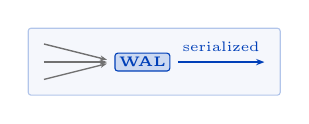
\begin{tikzpicture}[x=1cm,y=1cm]
      \draw[draw=pdcobalt!30,fill=pdcobalt!4,rounded corners=1pt] (0,0) rectangle (3.2,0.85);
      \draw[-{Stealth[length=2.5pt]},pdink!60,line width=0.5pt] (0.2,0.65) -- (1.0,0.45);
      \draw[-{Stealth[length=2.5pt]},pdink!60,line width=0.5pt] (0.2,0.42) -- (1.0,0.42);
      \draw[-{Stealth[length=2.5pt]},pdink!60,line width=0.5pt] (0.2,0.20) -- (1.0,0.40);
      \node[draw=pdcobalt,fill=pdcobalt!20,rounded corners=1pt,inner sep=1.5pt,font=\fontsize{4.5}{5.5}\selectfont\bfseries\color{pdcobalt}] at (1.45,0.42) {WAL};
      \draw[-{Stealth[length=3pt]},pdcobalt,line width=0.8pt] (1.9,0.42) -- (3.0,0.42) node[midway,above,font=\fontsize{4.2}{5.2}\selectfont\color{pdcobalt}] {serialized};
    \end{tikzpicture}%
  }{Arbitration: parallel writer attempts funnel into one causal sequence.}%
  Rules can be enforced before an act only when the system controls the channel through which the act
  occurs. Local effects therefore pass through one serial authority; semantic
  failures that no gate can decide remain matters of detection and remedy.

  \item \textbf{Delegation only narrows (\pdchapref{anchor}{The Anchor Protocol}).}%
  \pdmarginexhibit{anchor-attenuation}{Attenuation Cone}{%
    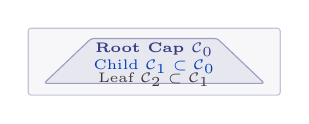
\begin{tikzpicture}[x=1cm,y=1cm]
      \draw[draw=pdindigo!30,fill=pdindigo!4,rounded corners=1pt] (0,0) rectangle (3.2,0.85);
      \draw[draw=pdindigo!50,fill=pdindigo!12,rounded corners=1pt] (0.2,0.15) -- (0.8,0.72) -- (2.4,0.72) -- (3.0,0.15) -- cycle;
      \node[font=\fontsize{4.5}{5.5}\selectfont\bfseries\color{pdindigo}] at (1.6,0.58) {Root Cap $\mathcal{C}_0$};
      \node[font=\fontsize{4.2}{5.2}\selectfont\color{pdcobalt}] at (1.6,0.36) {Child $\mathcal{C}_1 \subset \mathcal{C}_0$};
      \node[font=\fontsize{3.8}{4.8}\selectfont\color{pdinkmuted}] at (1.6,0.20) {Leaf $\mathcal{C}_2 \subset \mathcal{C}_1$};
    \end{tikzpicture}%
  }{Monotonic narrowing: delegated authority only diminishes at each hop.}%
  Every child capability is a strict subset of its parent's authority and lifetime. Authentication says who signed;
  attenuation says what the signature may authorize. Both are needed at every
  hop.

  \item \textbf{Confinement is a property of the room, not of the tenant (\pdchapref{sealed}{The Sealed Harbor}).}%
  \pdmarginexhibit{sealed-meter}{Egress Quota}{%
    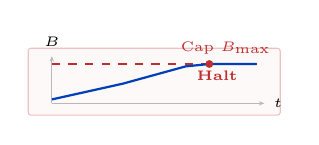
\begin{tikzpicture}[x=1cm,y=1cm]
      \draw[draw=pderror!30,fill=pderror!3,rounded corners=1pt] (0,0) rectangle (3.2,0.85);
      \draw[draw=pdink!30,line width=0.4pt,-{Stealth[length=2pt]}] (0.3,0.15) -- (3.0,0.15) node[right,font=\fontsize{3.5}{4.5}\selectfont] {$t$};
      \draw[draw=pdink!30,line width=0.4pt,-{Stealth[length=2pt]}] (0.3,0.15) -- (0.3,0.75) node[above,font=\fontsize{3.5}{4.5}\selectfont] {$B$};
      \draw[draw=pderror,line width=0.6pt,dashed] (0.3,0.65) -- (2.9,0.65) node[pos=0.85,above,font=\fontsize{3.8}{4.8}\selectfont\color{pderror}] {Cap $B_{\max}$};
      \draw[draw=pdcobalt,line width=0.8pt] (0.3,0.20) -- (1.2,0.40) -- (2.0,0.62) -- (2.3,0.65) -- (2.9,0.65);
      \node[circle,fill=pderror,inner sep=1pt] at (2.3,0.65) {};
      \node[font=\fontsize{3.8}{4.8}\selectfont\color{pderror}\bfseries] at (2.4,0.50) {Halt};
    \end{tikzpicture}%
  }{Spend ceiling: cumulative egress reaches cap $B_{\max}$ and halts execution.}%
  Two owners who trust neither each other nor the venue can still take one
  answer out of a sealed room when its only exit is a metered slot: silence
  except through the slot, a gate on the only enforceable boundary, a budget
  that conserves, and canaries for what the gate cannot prove. What the room
  cannot promise is stated as a limit, at the same prominence as the claims.

  \item \textbf{Supervision has an information cost (\pdchapref{ls}{Attention and Supervision}).}%
  \pdmarginexhibit{attention-entropy}{Rate-Distortion}{%
    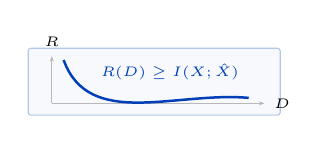
\begin{tikzpicture}[x=1cm,y=1cm]
      \draw[draw=pdcobalt!30,fill=pdcobalt!3,rounded corners=1pt] (0,0) rectangle (3.2,0.85);
      \draw[draw=pdink!30,line width=0.4pt,-{Stealth[length=2pt]}] (0.3,0.15) -- (3.0,0.15) node[right,font=\fontsize{3.5}{4.5}\selectfont] {$D$};
      \draw[draw=pdink!30,line width=0.4pt,-{Stealth[length=2pt]}] (0.3,0.15) -- (0.3,0.75) node[above,font=\fontsize{3.5}{4.5}\selectfont] {$R$};
      \draw[draw=pdcobalt,line width=0.9pt] (0.45,0.70) to[out=-70,in=175] (2.8,0.22);
      \node[font=\fontsize{4.2}{5.2}\selectfont\color{pdcobalt}] at (1.8,0.55) {$R(D) \ge I(X;\hat{X})$};
    \end{tikzpicture}%
  }{Information bound: lossy telemetry compression cannot bypass entropy rate.}%
  A digest cannot guarantee
  that a human will notice any one of many relevant events unless it spends
  enough bits, attention, or artifact openings to distinguish them. A summary
  is therefore an index into evidence, not a substitute for it.

  \item \textbf{Accountability must outlive the process (\pdchapref{stp}{From Spawn to Person}).}%
  \pdmarginexhibit{spawn-continuity}{Identity Lifeline}{%
    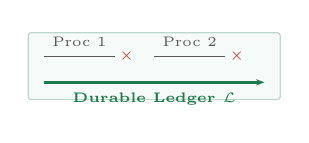
\begin{tikzpicture}[x=1cm,y=1cm]
      \draw[draw=pdhealth!30,fill=pdhealth!4,rounded corners=1pt] (0,0) rectangle (3.2,0.85);
      \draw[pdink!70,line width=0.6pt] (0.2,0.55) -- (1.1,0.55) node[pos=0.5,above,font=\fontsize{3.8}{4.8}\selectfont] {Proc 1};
      \node[font=\fontsize{4.5}{5.5}\selectfont\color{pderror}] at (1.25,0.55) {$\times$};
      \draw[pdink!70,line width=0.6pt] (1.6,0.55) -- (2.5,0.55) node[pos=0.5,above,font=\fontsize{3.8}{4.8}\selectfont] {Proc 2};
      \node[font=\fontsize{4.5}{5.5}\selectfont\color{pderror}] at (2.65,0.55) {$\times$};
      \draw[draw=pdhealth,line width=1.0pt,-{Stealth[length=3pt]}] (0.2,0.22) -- (3.0,0.22) node[pos=0.5,below,font=\fontsize{4.2}{5.2}\selectfont\color{pdhealth}\bfseries] {Durable Ledger $\mathcal{L}$};
    \end{tikzpicture}%
  }{Survivorship: transient process dies; case file and obligations persist.}%
  A task acquires a durable principal, capability history, evidence record, obligations, and
  outcome. Restarting an agent or choosing a new name must not erase that case
  file or refill the resources it already consumed.

  \item \textbf{Exchange requires separated instruments (\pdchapref{he}{The Harbor Economy}).}%
  \pdmarginexhibit{tx-instruments}{Four Instruments}{%
    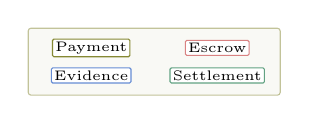
\begin{tikzpicture}[x=1cm,y=1cm]
      \draw[draw=pdgold!40,fill=pdgold!4,rounded corners=1pt] (0,0) rectangle (3.2,0.85);
      \node[draw=pdgold!80,fill=white,rounded corners=0.5pt,inner sep=1pt,font=\fontsize{3.8}{4.8}\selectfont] at (0.8,0.60) {Payment};
      \node[draw=pderror!60,fill=white,rounded corners=0.5pt,inner sep=1pt,font=\fontsize{3.8}{4.8}\selectfont] at (2.4,0.60) {Escrow};
      \node[draw=pdcobalt!60,fill=white,rounded corners=0.5pt,inner sep=1pt,font=\fontsize{3.8}{4.8}\selectfont] at (0.8,0.25) {Evidence};
      \node[draw=pdhealth!70,fill=white,rounded corners=0.5pt,inner sep=1pt,font=\fontsize{3.8}{4.8}\selectfont] at (2.4,0.25) {Settlement};
    \end{tikzpicture}%
  }{Separation: decoupling collateral from payout prevents moral hazard.}%
  Payment rewards the requested work. Collateral prices a bounded failure. Evidence supports a
  claim. Settlement closes it exactly once. Combining those functions in one
  score or token makes each of them less trustworthy.

  \item \textbf{Uncertainty needs an institution (\pdchapref{bonded}{The Bonded Commons}).}%
  \pdmarginexhibit{econ-reserves}{Bond Escrow}{%
    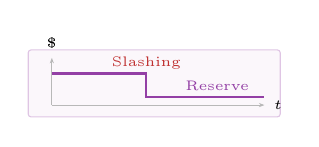
\begin{tikzpicture}[x=1cm,y=1cm]
      \draw[draw=pdviolet!30,fill=pdviolet!4,rounded corners=1pt] (0,0) rectangle (3.2,0.85);
      \draw[draw=pdink!30,line width=0.4pt,-{Stealth[length=2pt]}] (0.3,0.15) -- (3.0,0.15) node[right,font=\fontsize{3.5}{4.5}\selectfont] {$t$};
      \draw[draw=pdink!30,line width=0.4pt,-{Stealth[length=2pt]}] (0.3,0.15) -- (0.3,0.75) node[above,font=\fontsize{3.5}{4.5}\selectfont] {\$};
      \draw[draw=pdviolet,line width=0.8pt] (0.3,0.55) -- (1.5,0.55) -- (1.5,0.25) -- (3.0,0.25);
      \node[font=\fontsize{4}{5}\selectfont\color{pderror}] at (1.5,0.68) {Slashing};
      \node[font=\fontsize{4}{5}\selectfont\color{pdviolet}] at (2.4,0.40) {Reserve};
    \end{tikzpicture}%
  }{Collateral: breach of contract triggers deterministic slashing of bond.}%
  Some harms cannot be prevented and some outcomes cannot be judged mechanically. Witnesses,
  randomized audits, bounded bonds, appeals, and conservation rules turn that
  residual uncertainty into a process that can be inspected and contested.

  \item \textbf{Federation relays evidence, not sovereignty (\pdchapref{fh}{The Federated Harbor}).}%
  \pdmarginexhibit{fed-bridge}{Evidence Relay}{%
    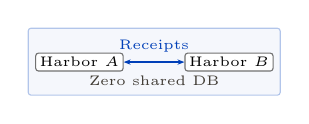
\begin{tikzpicture}[x=1cm,y=1cm]
      \draw[draw=pdcobalt!30,fill=pdcobalt!4,rounded corners=1pt] (0,0) rectangle (3.2,0.85);
      \node[draw=pdink!60,fill=white,rounded corners=1pt,inner sep=1.5pt,font=\fontsize{4}{5}\selectfont] (h1) at (0.65,0.42) {Harbor $A$};
      \node[draw=pdink!60,fill=white,rounded corners=1pt,inner sep=1.5pt,font=\fontsize{4}{5}\selectfont] (h2) at (2.55,0.42) {Harbor $B$};
      \draw[{Stealth[length=2.5pt]}-{Stealth[length=2.5pt]},pdcobalt,line width=0.7pt] (h1) -- (h2) node[midway,above,font=\fontsize{3.8}{4.8}\selectfont\color{pdcobalt}] {Receipts};
      \node[font=\fontsize{3.5}{4.5}\selectfont\color{pdinkmuted}] at (1.6,0.18) {Zero shared DB};
    \end{tikzpicture}%
  }{Federation: independent hosts exchange witness receipts, not sovereignty.}%
  Mutually distrustful machines may exchange signed capabilities, revocations, witness
  roots, and settlement claims without sharing a database or accepting a global
  ruler. Transport can carry evidence; it cannot decide what either machine is
  permitted to do with it.
\end{enumerate}

Read these as a dependency chain: each chapter uses earlier mechanisms and
states what they cannot guarantee.

\subsection{What Counts as Knowing: Epistemic Bounds and Evidence Channels}
\pdmarginfigure{lovelace}{Ada Lovelace observed that analytical engines have no pretensions to originate anything; they execute what we know how to order them to perform.}%
Every consequential statement in this volume has a status and a boundary. Derivations establish
relations under named assumptions. Finite checks exhaust a stated state space,
not every deployment. Simulations estimate behavior under a stated generator;
repository tests exercise named paths; running code proves availability, not
universal mediation. Counterexamples remain in the record because they mark
claims the research killed rather than conclusions it merely failed to prove.

Evidence is typed as well. When a chapter reports what a harbor observed, it
names the channel that produced the observation, and each channel has a blind
spot that no amount of volume removes:
\begin{itemize}[leftmargin=1.8em,itemsep=2pt]
  \item A \emph{deterministic verifier} (a test, a type checker, a model checker) shows that a stated property holds of the artifact it examined, and nothing about properties it did not state.
  \item A \emph{provenance witness} (a signature, a hash, a Merkle inclusion, an append-only log) shows attribution and tamper-evidence relative to a commitment, never that every event was logged or that a description is true.
  \item A \emph{protected meter} (a counter its subject cannot rewrite) shows a quantity, not its cause.
  \item \emph{Expert judgment} shows an assessment under a named rubric and carries the assessor's error rate.
  \item \emph{Buyer preference} shows what was chosen, not that the choice was right.
  \item A \emph{delayed outcome} shows what happened, and arrives too late to prevent it.
\end{itemize}
The reader should ask the same question of any dashboard: which channel, and what can it not show.

\Cref{app:volume-status} gives the implementation boundary;
\cref{app:result-atlas} records the results and their limits. The companion
\path{docs/harbor-research/mega-volume-epistemic-manifest.yaml} preserves each
result's source, status, conditions, boundary, chapter home, and verification
artifact. The chapters stand alone; the book's claim is the chain they make.

\section{Classical Multi-Agent Systems Foundations}\label{sec:prereq-classical-mas}

Before analyzing neural coding agents, we formalize the foundational frameworks developed during the classical era of multi-agent systems.

\subsection{Intentional Agency and Practical Rationality}

Classical decision theory models an agent as an expected utility maximizer balancing subjective beliefs $\mathcal{B}$ and desires $\mathcal{D}$. In his seminal 1987 work \emph{Intention, Plans, and Practical Reason}, philosopher Michael Bratman demonstrated that this two-component model is computationally inadequate for resource-bounded agents operating in dynamic environments~\pdcite{bratman1987intention}.

A resource-bounded agent cannot continuously compute optimal policies from first principles at every millisecond. Practical rationality requires a third mental attitude: \textbf{Intention} ($\mathcal{I}$). Intentions are not merely desires with high utility; they represent \emph{conduct-controlling pro-attitudes to which the agent has actively committed}.

Bratman established four defining functional roles of intentions:
\begin{enumerate}[leftmargin=1.8em,itemsep=2pt]
  \item \textbf{Drive Means-End Reasoning:} An intention to achieve goal $\phi$ obligates the agent to formulate sub-plans and allocate computational cycles until $\phi$ is satisfied.
  \item \textbf{Filter of Admissibility:} Once an intention $\phi$ is adopted, candidate options inconsistent with $\phi$ (given current beliefs $\mathcal{B}$) are ruled inadmissible without evaluating their cost-benefit payoff.
  \item \textbf{Stability and Commitment:} Intentions resist reconsideration in the absence of relevant environmental interrupts or belief updates, preventing computational paralysis.
  \item \textbf{Coordination Scaffolding:} Intentions enable interpersonal coordination: other agents can safely form expectations regarding an agent's future actions based on its declared commitments.
\end{enumerate}

\subsection{The Rao--Georgeff BDI Temporal Logic (\texorpdfstring{$BDI_{CTL^*}$}{BDI-CTL*})}

Rao and Georgeff~\pdcite{rao1991modeling,rao1995bdi} formalized Bratman's theory into a multimodal branching-time temporal logic ($BDI_{CTL^*}$). A temporal world model $\mathcal{M}$ is defined as an 8-tuple:
\begin{equation}
\mathcal{M} \;=\; \langle W, T, \prec, U, \mathcal{B}, \mathcal{D}, \mathcal{I}, \Phi \rangle
\end{equation}
where $W$ is a set of possible worlds, $T$ is a discrete set of time points ordered by tree-branching relation $\prec$, $U$ is the universe of discourse, $\Phi$ interprets predicates across worlds and times, and $\mathcal{B}, \mathcal{D}, \mathcal{I} \subseteq W \times T \times W$ are accessibility relations for Beliefs, Desires, and Intentions.

For world $w \in W$ at time $t \in T$:
\begin{align}
\mathcal{B}_t(w) &= \{ w' \in W \mid (w, t, w') \in \mathcal{B} \} \\
\mathcal{D}_t(w) &= \{ w' \in W \mid (w, t, w') \in \mathcal{D} \} \\
\mathcal{I}_t(w) &= \{ w' \in W \mid (w, t, w') \in \mathcal{I} \}
\end{align}

Semantics of the mental modalities at state $\langle w, t \rangle$:
\begin{align}
\mathcal{M}, w, t \models \mathrm{Bel}(\phi) &\iff \forall w' \in \mathcal{B}_t(w), \; \mathcal{M}, w', t \models \phi \\
\mathcal{M}, w, t \models \mathrm{Des}(\phi) &\iff \forall w' \in \mathcal{D}_t(w), \; \mathcal{M}, w', t \models \phi \\
\mathcal{M}, w, t \models \mathrm{Int}(\phi) &\iff \forall w' \in \mathcal{I}_t(w), \; \mathcal{M}, w', t \models \phi
\end{align}

Beliefs satisfy the $KD45$ axiom system (deductive closure $\mathbf{K}$, consistency $\mathbf{D}$, positive introspection $\mathbf{4}$, and negative introspection $\mathbf{5}$). Desires and Intentions satisfy seriality ($\mathbf{D}$), ensuring an agent never desires or intends logical contradictions ($\neg\mathrm{Des}(\bot)$ and $\neg\mathrm{Int}(\bot)$).

\subsubsection{Compatibility and Weak Realism}
In rational agency, an agent's desires and intentions must be constrained by its beliefs. Under the \textbf{Weak Realism} axiom, an agent cannot intend what it believes to be impossible:
\begin{equation}
\forall w \in W, \; \mathcal{I}_t(w) \cap \mathcal{B}_t(w) \neq \emptyset
\end{equation}
Syntactically, for temporal achievement goals:
\begin{equation}
\mathrm{Int}(\mathbf{A}\lozenge \phi) \;\to\; \neg\mathrm{Bel}(\neg\mathbf{E}\lozenge \phi)
\end{equation}
where $\mathbf{A}\lozenge \phi$ denotes ``$\phi$ holds eventually on all future paths,'' and $\mathbf{E}\lozenge \phi$ denotes ``$\phi$ holds on at least one branch.''

\subsection{Formal Commitment Strategies}

A commitment strategy dictates the precise formal conditions under which an agent drops an intention $\phi$. Rao and Georgeff~\pdcite{rao1991modeling} formalized three canonical strategies:

\begin{table}[H]
\centering
\small
\begin{tabularx}{\textwidth}{lX}
\toprule
\textbf{Commitment Strategy} & \textbf{Formal Drop Axiom} \\
\midrule
\textbf{Blind (Fanatical)} & Maintains $\mathrm{Int}(\mathbf{A}\lozenge \phi)$ until $\mathrm{Bel}(\phi)$ holds. \\
& $\mathrm{Int}(\mathbf{A}\lozenge \phi) \land \neg\mathrm{Bel}(\phi) \to \mathbf{A}\big(\mathrm{Int}(\mathbf{A}\lozenge \phi) \;\mathcal{U}\; \mathrm{Bel}(\phi)\big)$. \\
& \emph{Pathology:} Induces infinite loops if $\phi$ becomes physically impossible. \\
\addlinespace[3pt]
\textbf{Single-Minded} & Drops $\phi$ if achieved \emph{or} believed impossible. \\
& $\mathrm{Int}(\mathbf{A}\lozenge \phi) \land \neg\mathrm{Bel}(\phi) \land \mathrm{Bel}(\mathbf{E}\lozenge \phi) \to \mathbf{A}\big(\mathrm{Int}(\mathbf{A}\lozenge \phi) \;\mathcal{U}\; (\mathrm{Bel}(\phi) \lor \neg\mathrm{Bel}(\mathbf{E}\lozenge \phi))\big)$. \\
& \emph{Standard:} Balances persistence with dynamic feasibility. \\
\addlinespace[3pt]
\textbf{Open-Minded} & Drops $\phi$ if achieved, impossible, \emph{or no longer desired}. \\
& $\mathrm{Int}(\mathbf{A}\lozenge \phi) \land \dots \land \mathrm{Des}(\mathbf{A}\lozenge \phi) \to \mathbf{A}\big(\mathrm{Int}(\mathbf{A}\lozenge \phi) \;\mathcal{U}\; (\mathrm{Bel}(\phi) \lor \neg\mathrm{Bel}(\mathbf{E}\lozenge \phi) \lor \neg\mathrm{Des}(\mathbf{A}\lozenge \phi))\big)$. \\
\bottomrule
\end{tabularx}
\caption{Canonical commitment strategies in BDI agent architectures.}
\label{tab:commitment-strategies}
\end{table}

\begin{pdclaim}{Design invariant}{Commitment Persistence}\label{inv:commitment-persistence}
An agent's intention $\iota \in \mathcal{I}$ must not be abandoned merely because a single step incurs a transient tool failure. Intention reconsideration is an explicit state transition triggered by invariant failure or objective discharge, not an accidental consequence of context window truncation.
\end{pdclaim}

\subsection{Operational Semantics of AgentSpeak(L) and Normative Extensions}

AgentSpeak(L)~\pdcite{bordini2007agentspeak} provides structural operational semantics (SOS) for executing BDI agents. An agent configuration is a tuple $C = \langle bs, ps, is, \mathcal{E}, A \rangle$, where $bs$ is the belief base, $ps$ is the plan library, $is$ is the set of active intention stacks, $\mathcal{E}$ is the event queue, and $A$ is the action history.

The operational execution cycle is governed by three deterministic or priority-driven selection functions:
\begin{enumerate}[leftmargin=1.8em,itemsep=2pt]
  \item $S_E(\mathcal{E}) = \langle te, i \rangle$: Selects an event from $\mathcal{E}$ (e.g., belief change $+b$, goal addition $+!g$).
  \item $S_O(\mathrm{App})$: Selects a plan $(p, \theta)$ from the applicable plans whose context is entailed by $bs\theta$.
  \item $S_I(is) = i$: Selects which intention stack advances its execution step in the current cycle.
\end{enumerate}

When an action $a$ in plan $p$ fails during host execution, AgentSpeak semantics do not silently abort the agent; instead, the failure transition posts a failure event $-!g$ to $\mathcal{E}$, popping the failed plan frame and invoking explicit recovery plans:
\begin{equation}
\frac{\epsilon = \langle te, i \rangle, \quad \mathrm{App}(\mathrm{Rel}(te, ps), bs) = \emptyset}{\langle bs, ps, is, \mathcal{E}, A \rangle \;\longrightarrow\; \langle bs, ps, is, \mathcal{E} \cup \{\langle -!g, \mathrm{pop}(i) \rangle\}, A \rangle}
\end{equation}

Figure~\ref{fig:bdi-execution-flow} synthesizes this operational choice architecture, illustrating how autonomous systems select between reactive rules, static classical planning, and BDI execution, and how $S_E, S_O$, and $S_I$ arbitrate runtime goals.

\begin{figure}[p]
\centering
\definecolor{swissCanvas}{HTML}{F8F9FA}     % Neutral canvas ground
\definecolor{charcoal}{HTML}{1A1A1A}        % Structural boundaries & primary text
\definecolor{activeCobalt}{HTML}{0B4F9C}    % Selected paradigm & active intention commit
\definecolor{activeTint}{HTML}{E8F0FE}      % Active deliberation frame fill
\definecolor{seafoamSuccess}{HTML}{D1E7DD}  % Nominal progression (Exit 0)
\definecolor{seafoamBorder}{HTML}{0F5132}   % Success accent
\definecolor{coralRecovery}{HTML}{F8D7DA}   % Failure trap & recovery (-!g, Exit != 0)
\definecolor{coralBorder}{HTML}{842029}     % Recovery accent
\definecolor{ingressTint}{HTML}{EEF4C7}     % Requirement / External input specification

\begin{tikzpicture}[pd figure,x=1cm,y=1cm,
  >=Stealth,
  baseBox/.style={
    draw=charcoal, line width=0.8pt, fill=white, text=charcoal,
    inner sep=5pt, align=left, font=\footnotesize
  },
  gridBox/.style={
    baseBox, text width=3.6cm, minimum height=1.35cm
  },
  activeBox/.style={
    gridBox, draw=activeCobalt, fill=activeCobalt, text=white
  },
  successBox/.style={
    baseBox, draw=seafoamBorder, fill=seafoamSuccess, text=charcoal, text width=4.8cm, minimum height=1.3cm
  },
  recoveryBox/.style={
    baseBox, draw=coralBorder, fill=coralRecovery, text=charcoal, text width=4.8cm, minimum height=1.3cm
  },
  sectionFrame/.style={
    draw=charcoal, line width=0.9pt
  },
  secHeader/.style={
    font=\bfseries\footnotesize, text=charcoal, anchor=west
  }
]
  \useasboundingbox (0, 0.2) rectangle (15.5, 18.8);

  % ================= HEADER & SEMANTIC KEY =================
  \node[anchor=west, font=\bfseries\normalsize, text=charcoal] at (0.2, 18.4) {BDI AGENT OPERATIONAL CONCURRENCY ARCHITECTURE};
  \node[anchor=west, font=\footnotesize, text=charcoal] at (0.2, 17.95) {AgentSpeak(L) Operational Cycle \textperiodcentered\ Rao--Georgeff State Transition System};
  \node[anchor=east, font=\bfseries\footnotesize, text=charcoal] at (15.3, 17.95) {RAO \& GEORGEFF (1995)};
  \draw[line width=1.2pt, charcoal] (0.2, 17.7) -- (15.3, 17.7);

  % Semantic Key
  \node[anchor=west, font=\footnotesize\bfseries, text=charcoal] at (0.2, 17.35) {SEMANTIC KEY:};
  
  \node[anchor=west, draw=charcoal, fill=ingressTint, line width=0.6pt, minimum width=0.35cm, minimum height=0.25cm] at (2.6, 17.35) {};
  \node[anchor=west, font=\footnotesize, text=charcoal] at (3.05, 17.35) {Problem Spec};

  \node[anchor=west, draw=activeCobalt, fill=activeCobalt, line width=0.6pt, minimum width=0.35cm, minimum height=0.25cm] at (5.7, 17.35) {};
  \node[anchor=west, font=\footnotesize, text=charcoal] at (6.15, 17.35) {Active Deliberation};

  \node[anchor=west, draw=seafoamBorder, fill=seafoamSuccess, line width=0.6pt, minimum width=0.35cm, minimum height=0.25cm] at (9.4, 17.35) {};
  \node[anchor=west, font=\footnotesize, text=charcoal] at (9.85, 17.35) {Nominal (Exit 0)};

  \node[anchor=west, draw=coralBorder, fill=coralRecovery, line width=0.6pt, minimum width=0.35cm, minimum height=0.25cm] at (12.7, 17.35) {};
  \node[anchor=west, font=\footnotesize, text=charcoal] at (13.15, 17.35) {Failure Trap ($-!g$)};

  % ================= SECTION 1: PARADIGM SELECTION =================
  \draw[sectionFrame] (0.2, 11.75) rectangle (15.3, 17.15);
  \node[secHeader] at (0.45, 16.7) {1. ARCHITECTURAL PARADIGM SELECTION (GOAL DYNAMICS VS INTERRUPT ABSORPTION)};

  % Autonomous Requirement Specification
  \node[baseBox, fill=ingressTint, text width=9.2cm, align=center, anchor=north] (req) at (7.75, 16.65) {
    \textbf{\footnotesize Autonomous Behavior Requirement} \\[1pt]
    \footnotesize Ex: \texttt{"Refactor auth middleware to JWT \& pass CI test suite"}
  };

  % Decision Splitter
  \node[baseBox, draw=charcoal, line width=0.9pt, text width=6.6cm, align=center, anchor=north] (decision) at (7.75, 15.35) {
    \textbf{\footnotesize Persistent goals plus interrupts?} \\[1pt]
    \footnotesize Dynamic replanning \& recovery needed?
  };
  \draw[->, line width=1.0pt, charcoal] (req.south) -- (decision.north);

  % Three Columns of Architectures (anchor=north at y = 13.6, text width=3.6cm)
  \node[gridBox, anchor=north] (reactive) at (2.2, 14.15) {
    \textbf{Reactive Rules} \\[2pt]
    \footnotesize Event-condition-action \\[1pt]
    \footnotesize\texttt{on\_busy $\to$ kill(pid)} \\[1pt]
    \footnotesize No persistent goals
  };

  \node[gridBox, anchor=north] (classical) at (7.75, 14.15) {
    \textbf{Classical Planner} \\[2pt]
    \footnotesize Static STRIPS / HTN \\[1pt]
    \footnotesize Brittle to tool failures \\[1pt]
    \footnotesize Cannot handle interrupts
  };

  \node[activeBox, anchor=north] (bdi) at (13.3, 14.15) {
    \textbf{BDI Architecture} \\[2pt]
    \footnotesize Beliefs, Plans, Intentions \\[1pt]
    \footnotesize Dynamic deliberation \\[1pt]
    \footnotesize Goal persistence \& recovery
  };

  % Connectors
  \draw[->, line width=1.0pt, charcoal] (decision.west) -| (reactive.north)
    node[pos=0.4, above=2pt, font=\footnotesize\bfseries] {No interrupts};
  \draw[->, line width=1.0pt, charcoal] (decision.south) -- (classical.north)
    node[midway, fill=white, inner sep=1.5pt, font=\footnotesize\bfseries] {Static goals};
  \draw[->, line width=1.1pt, activeCobalt] (decision.east) -| (bdi.north)
    node[pos=0.4, above=2pt, font=\footnotesize\bfseries, text=activeCobalt] {Goals + Interrupts};

  % ================= SECTION 2: DELIBERATION CYCLE =================
  \draw[sectionFrame, draw=activeCobalt, line width=1.3pt, fill=activeTint!25] (0.2, 0.3) rectangle (15.3, 11.55);
  \node[secHeader, text=activeCobalt] at (0.45, 11.2) {2. AGENTSPEAK(L) OPERATIONAL DELIBERATION CYCLE (STATE TRANSITIONS)};

  % Row 1: Deliberation Steps (anchor=north at y = 10.6)
  \node[gridBox, draw=activeCobalt, anchor=north] (step1) at (2.2, 10.5) {
    \textbf{1. Event Selection ($S_E$)} \\[2pt]
    \footnotesize Pop event from queue $\mathcal{E}$: \\[2pt]
    \footnotesize$\langle +!g_{\text{build}}, i_{\text{auth}} \rangle \leftarrow S_E(\mathcal{E})$
  };

  \node[gridBox, draw=activeCobalt, anchor=north] (step2) at (7.75, 10.5) {
    \textbf{2. Plan Selection ($S_O$)} \\[2pt]
    \footnotesize Match context: $\text{App} \subseteq \mathcal{P}$ \\[2pt]
    \footnotesize Select: $p_{\text{jwt}} \leftarrow S_O(\text{App})$
  };

  \node[activeBox, anchor=north] (step3) at (13.3, 10.5) {
    \textbf{3. Intention Selection ($S_I$)} \\[2pt]
    \footnotesize Schedule: $i_{\text{auth}} \leftarrow S_I(\mathcal{I})$ \\[2pt]
    \footnotesize\textbf{Commit slice to stack}
  };

  % Row 1 Connectors with clean raised labels
  \draw[->, line width=1.0pt, charcoal] (step1.east) -- (step2.west)
    node[midway, above=2pt, font=\footnotesize\bfseries, text=charcoal] {Relevant};
  \draw[->, line width=1.0pt, activeCobalt] (step2.east) -- (step3.west)
    node[midway, above=2pt, font=\footnotesize\bfseries, text=activeCobalt] {Applicable};

  % Row 2: Ingestion, Status, and Commitment (anchor=north at y = 7.4)
  \node[gridBox, anchor=north] (queue) at (2.2, 7.4) {
    \textbf{Queue Ingestion} \\[2pt]
    \footnotesize Enqueue subgoals $+!g$ \\[1pt]
    \footnotesize Enqueue beliefs $+b$
  };

  \node[baseBox, draw=charcoal, line width=0.9pt, text width=3.8cm, align=center, anchor=north] (status) at (7.75, 7.4) {
    \textbf{\footnotesize Execution Status Check} \\[2pt]
    \footnotesize Environmental exit code\\[1pt]
    \footnotesize Verify sandbox result
  };

  \node[gridBox, anchor=north] (commit) at (13.3, 7.4) {
    \textbf{Commitment Review} \\[2pt]
    \footnotesize Check drop conditions \\[1pt]
    \footnotesize Prevent goal thrashing
  };

  % Row 2 Connectors
  \draw[->, line width=1.1pt, activeCobalt] (step3.south) -- (commit.north);
  \draw[->, line width=1.0pt, charcoal] (commit.west) -- (status.east);
  \draw[->, line width=1.0pt, charcoal] (queue.north) -- (step1.south)
    node[midway, right=3pt, font=\footnotesize\bfseries] {New Cycle};

  % Row 3: Outcomes & Recovery (anchor=north at y = 4.1)
  \node[recoveryBox, anchor=north] (recovery) at (4.8, 4.1) {
    \textbf{\footnotesize Post $-!g$ Recovery} \\[2pt]
    \footnotesize Pop failed intention stack frame; \\[1pt]
    \footnotesize Post failure event $-!g$ to queue $\mathcal{E}$
  };

  \node[successBox, anchor=north] (advance) at (10.7, 4.1) {
    \textbf{\footnotesize Advance Intention} \\[2pt]
    \footnotesize Push validated plan body to $i_{\text{auth}}$; \\[1pt]
    \footnotesize Execute next action in slice
  };

  % Split Branching from Status Check
  \draw[line width=1.0pt, charcoal] (7.75, 5.9) -- (7.75, 4.9);

  % Exit != 0 branch (Left)
  \draw[->, line width=1.1pt, coralBorder] (7.75, 4.9) -| (recovery.north)
    node[pos=0.35, above=2pt, font=\footnotesize\bfseries, text=coralBorder] {Exit $\neq 0$ (Failure)};

  % Exit = 0 branch (Right)
  \draw[->, line width=1.1pt, seafoamBorder] (7.75, 4.9) -| (advance.north)
    node[pos=0.35, above=2pt, font=\footnotesize\bfseries, text=seafoamBorder] {Exit $= 0$ (Nominal)};

  % Recovery Feedback Loop (Clean left gutter at x = 0.45)
  \draw[->, line width=1.1pt, coralBorder, dashed] (recovery.west) -- (0.45, 3.45) |- (queue.west)
    node[pos=0.25, left=1pt, font=\footnotesize\bfseries, text=coralBorder] {$-!g$ Trigger};

  % Advance Intention Loopback (Clean right gutter at x = 15.05)
  \draw[->, line width=1.1pt, seafoamBorder] (advance.east) -- (15.05, 3.45) |- (commit.east)
    node[pos=0.25, right=1pt, font=\footnotesize\bfseries, text=seafoamBorder] {Next Slice};

  % Deliberation Invariant Footer Box (anchor=north at y = 1.9)
  \node[baseBox, text width=14.4cm, align=center, inner sep=5pt, anchor=north] at (7.75, 1.9) {
    \textbf{Operational Cycle Invariant $\mathcal{I}_{\text{BDI}}$:} $\forall t, \;\mathcal{E}_{t+1} = \big(\mathcal{E}_t \setminus \{e\}\big) \cup \mathsf{ExtEvents} \cup \mathsf{IntSubgoals}$.\\[2pt]
    Intention commitments persist across clock ticks until explicitly achieved or dropped by commitment review.
  };

\end{tikzpicture}
\caption{BDI execution flow and operational choice architecture, grounded in real-world software engineering workflows. Adapted from AgentSpeak(L) semantics~\pdcite{bordini2007agentspeak}, contrasting reactive rule triggers, static STRIPS-style planners, and dynamic BDI agents. The three core selection functions ($S_E$ for events, $S_O$ for applicable plans, and $S_I$ for intention stacks) arbitrate runtime goal scheduling, with explicit plan failure handling via the $-!g$ recovery event.}
\label{fig:bdi-execution-flow}
\end{figure}
\pdmarginpagebreak

\subsubsection{Normative Extensions: Deontic Constraints and Regret Minimization}
In institutional multi-agent systems, agents are constrained by external \textbf{norms} (deontic logic). A norm is defined as a 6-tuple $N = \langle \text{id}, \text{Type}, \phi_{\text{act}}, \phi_{\text{tgt}}, d, \text{Sanction} \rangle$, where $\text{Type} \in \{\mathcal{O}, \mathcal{F}, \mathcal{P}\}$ (Obligation, Prohibition, Permission), $\phi_{\text{act}}$ is the activation context, $\phi_{\text{tgt}}$ is the target state, $d$ is the deadline, and $\text{Sanction}$ is the penalty for violation.

To reconcile institutional norms with internal intentions, agents maintain an \textbf{Abstract Norm Base} ($ANB$) and evaluate instantiated norms in the \textbf{Norm Instance Base} ($NIB$). When norm instances conflict with active goals ($Plans(is \cup \mathcal{N}) = \emptyset$), the agent resolves the normative conflict by partitioning candidate norms into \textbf{Maximal Non-Conflicting Subsets} (MNCS), selecting the subset that minimizes maximum penalty under a \textbf{minimax regret} criterion:
\begin{equation}
S^* \;=\; \arg\min_{S \in \Omega} \;\max_{n_v \in \mathcal{N} \setminus S} \;\mathrm{Cost}(\mathrm{Sanction}(n_v))
\end{equation}
This ensures that any deliberate norm violation is recorded in an immutable ledger alongside its formal justification.

\subsection{Concurrency: Hewitt--Agha Actor Model vs. Hoare CSP}

Multi-agent coordination requires formal concurrency models. Classical computer science produced two foundational, mathematically rigorous paradigms for message-passing concurrency: the \textbf{Hewitt--Agha Actor Model}~\pdcite{hewitt1973actor,agha1986actors} and C.~A.~R.~Hoare's \textbf{Communicating Sequential Processes (CSP)}~\pdcite{hoare1978csp}. While both reject shared mutable memory in favor of message passing, their underlying abstractions of identity, synchronization, buffering, and failure isolation represent fundamentally divergent philosophies of distributed computation.

\begin{table}[H]
\centering
\small
\begin{tabularx}{\textwidth}{lXX}
\toprule
\textbf{Dimension} & \textbf{Hewitt--Agha Actor Model~\pdcite{hewitt1973actor,agha1986actors}} & \textbf{Hoare's CSP (1978)~\pdcite{hoare1978csp}} \\
\midrule
\textbf{Primitive} & Autonomous Actor with private state & Sequential Process and Named Channel \\
\textbf{Synchronization} & Asynchronous (non-blocking send) & Synchronous (rendezvous handshake) \\
\textbf{Addressing} & First-class Mailbox addresses & Explicit Channel identifiers \\
\textbf{Buffering} & Unbounded mailbox queue & Zero buffer (unbuffered channels) \\
\textbf{State Evolution} & Replacement behavior ($\mathtt{become}(B')$) & Sequential instruction trace \\
\textbf{Failure Mode} & Mailbox overflow; unhandled messages & Circular rendezvous deadlock \\
\textbf{Modern Descendant} & Erlang/OTP, Akka, Ray, agentsd & Go channels, Rust crossbeam \\
\bottomrule
\end{tabularx}
\caption{Message-passing concurrency: Hewitt--Agha actors versus Hoare CSP.}
\label{tab:concurrency-models}
\end{table}

\subsubsection{Mathematical Semantics of Actor Execution}
In the Actor model, an actor $\alpha \in \mathcal{A}$ is an autonomous computational entity encapsulating a private state $S \in \mathcal{S}$ and an incoming message mailbox $\mathcal{Q} \in \mathcal{M}^*$. Crucially, an actor possesses zero shared memory with any peer. When an actor dequeues a message $m \in \mathcal{M}$ from its mailbox, it evaluates an atomic transition function:
\begin{equation}
\mathrm{Actor}(S, m) \;\xrightarrow{\text{atomic}}\; \big\langle S',\; \mathcal{M}_{\mathrm{out}},\; \mathcal{A}_{\mathrm{spawn}} \big\rangle
\end{equation}
where:
\begin{enumerate}[leftmargin=1.8em,itemsep=1pt]
  \item $S' = \mathtt{become}(B')$ designates the actor's \emph{replacement behavior}—the state and logic that will govern the consumption of the subsequent message $m_{t+1}$.
  \item $\mathcal{M}_{\mathrm{out}} = \{ \langle \mathtt{addr}_k, v_k \rangle \}_{k=1}^n$ is a finite set of asynchronous outbound messages dispatched to known recipient addresses.
  \item $\mathcal{A}_{\mathrm{spawn}} = \{ \alpha_{\mathrm{new}, 1}, \dots, \alpha_{\mathrm{new}, j} \}$ is a finite set of newly created actor instances, each endowed with a fresh cryptographic identity and private state.
\end{enumerate}
Because message dispatch is strictly asynchronous and non-blocking ($\mathtt{send}$ returns instantaneously), the sender never waits for the receiver to process the payload. This decouples communicating actors across both space and time.

\subsubsection{Mathematical Semantics of CSP Synchronous Rendezvous}
In contrast, Hoare's Communicating Sequential Processes formalizes concurrency as an algebra of sequential processes interacting via unbuffered, named communication channels $c \in \mathcal{C}$. Communication is modeled in labeled transition systems as a synchronous, atomic event requiring mutual agreement:
\begin{equation}
\frac{P_1 \;\xrightarrow{c!v}\; P_1' \quad\quad P_2 \;\xrightarrow{c?x}\; P_2'[x \mapsto v]}{P_1 \parallel P_2 \;\xrightarrow{\tau}\; P_1' \parallel P_2'}
\end{equation}
In this operational rule:
\begin{itemize}[leftmargin=1.8em,itemsep=1pt]
  \item Process $P_1$ executes the output command $c!v$ (send value $v$ on channel $c$) and immediately blocks.
  \item Process $P_2$ executes the input command $c?x$ (receive into variable $x$ on channel $c$) and blocks until a sender arrives.
  \item The interaction is an instantaneous rendezvous: the value $v$ is transferred into $x$ without intermediate buffering ($|c| = 0$), and both $P_1$ and $P_2$ unblock simultaneously at the exact same physical clock tick ($\Delta t = 0$), emitting the internal transition $\tau$.
\end{itemize}

\subsubsection{Comparative Architectural Analysis}
Understanding the operational distinction between these two models is essential for architecting multi-agent developer workflows:

\begin{enumerate}[leftmargin=1.8em,itemsep=3pt]
  \item \textbf{Addressing and Coupling:} In the Actor model, communication is identity-centric: an actor addresses messages to a destination mailbox reference ($\mathtt{send}(\alpha_{\mathrm{worker}}, m)$). Senders and receivers can be dynamically reconfigured, migrated across physical nodes, or restarted without altering the message protocol. In CSP, communication is channel-centric: processes are anonymous to one another and couple exclusively through named conduits ($c!v$). This affords strong compile-time verification of dataflow graphs, but makes dynamic runtime topology discovery more rigid.
  
  \item \textbf{Temporal Coupling and Latency Variance:} In CSP, synchronous rendezvous enforces strict temporal lockstep. If process $P_1$ attempts to output to $P_2$, but $P_2$ is occupied with compute, $P_1$ is paralyzed until $P_2$ completes its work. In contrast, the Actor model completely decouples temporal execution: $P_1$ deposits the message in $P_2$'s mailbox and immediately resumes local progress.
  
  \item \textbf{State Evolution and Concurrency Safety:} In CSP, processes evolve through an imperative trace of sequential instructions interspersed with channel choices ($P = c?x \to Q(x) \mathbin{\square} d?y \to R(y)$). In the Actor model, state evolution is explicitly functional: an actor never mutates internal state concurrently; instead, it executes the $\mathtt{become}$ primitive, atomically rebinding its message-processing closure for the next dequeued event.
  
  \item \textbf{Failure Semantics and Fault Domains:} The fatal failure mode of CSP is \textbf{circular wait deadlock}: if $P_1$ waits to output on channel $c_1$ to $P_2$, while $P_2$ waits to output on channel $c_2$ to $P_1$, the entire system permanently halts. In the Actor model, circular deadlock on send is structurally impossible because sends never block. However, actors face two distinct hazards: \emph{mailbox overflow} (an actor receiving messages faster than it can process them) and \emph{silent failure} (a crashed actor abandoning unhandled messages). Erlang/OTP resolved this by introducing hierarchical \textbf{supervision trees}: actors are monitored by supervisors operating under a ``let it crash'' philosophy, restarting failed workers from clean initial states.
\end{enumerate}

\subsubsection{Architectural Implications for Autonomous Agent Operating Systems}
When deploying autonomous LLM agents (such as Codex, Claude, or local reasoning models) to perform real-world software engineering, naive concurrency models fail:

\begin{itemize}[leftmargin=1.8em,itemsep=2pt]
  \item \textbf{Why LLM Fleets Cannot Use Pure Synchronous CSP:} Language model inference is inherently stochastic and long-running, with single tool-invocation latencies spanning seconds to minutes. If an orchestrator agent engaged in synchronous CSP rendezvous with child worker agents, the orchestrator's event loop would freeze entirely during child inference. If two agents attempted mutual queries, the swarm would instantly deadlock.
  \item \textbf{Why Naive Unbounded Mailboxes Cause Agentic Collapse:} Conversely, if agents are implemented with unmetered actor mailboxes, asynchronous message flooding causes catastrophic context-window saturation. An agent receiving twenty interleaved status updates during a build tool call will exhaust its prompt token budget upon mailbox drain, inducing hallucinatory drift.
  \item \textbf{The Agent OS Synthesis:} A robust operating kernel therefore synthesizes both lineages:
  \begin{enumerate}[leftmargin=1.4em,itemsep=1pt]
    \item \emph{Actor Encapsulation for Execution Sandboxes:} Each autonomous worker is an isolated Actor running in a seatbelted OS process with private memory, an attenuated capability key, and an append-only evidence mailbox.
    \item \emph{CSP and Linda Tuple Spaces for Physical Synchronization:} Contention over scarce physical resources (TCP port claims, SQLite write-ahead log commits, and git branch locks) is arbitrated through synchronous rendezvous barriers with mandatory lease timeouts, preventing deadlocks while guaranteeing mutual exclusion.
  \end{enumerate}
\end{itemize}

Figure~\ref{fig:actor-concurrency} details the Hewitt--Agha virtual actor concurrency architecture, while Figure~\ref{fig:csp-concurrency} articulates Hoare's Communicating Sequential Processes (CSP) synchronous rendezvous, guarded external choice, and deadlock resolution mechanics.

\pdmarginanalogy{prereq-token-staff}{}{ch01-railway-token-staff}{Like the physical railway token staff that guarantees exclusive single-track authority, an actor holds sovereign right over its private mailbox and sequential state transitions.}%
\begin{figure}[p]
\centering
\definecolor{swissCanvas}{HTML}{F8F9FA}     % Neutral canvas ground
\definecolor{charcoal}{HTML}{1A1A1A}        % Structural boundaries & invariants
\definecolor{ingressTint}{HTML}{EEF4C7}     % Ingress: External boundary & input dispatch
\definecolor{activeCobalt}{HTML}{0B4F9C}    % Active: Mutating execution & hot-path message
\definecolor{activeTint}{HTML}{E8F0FE}      % Active Container Fill
\definecolor{remedySeafoam}{HTML}{D1E7DD}   % Recovery: Fault isolation & supervisory remedy
\definecolor{remedyBorder}{HTML}{0F5132}    % Supervisory Accent
\definecolor{codeBg}{HTML}{EBECEF}          % Durable evidence record

\begin{tikzpicture}[pd figure,x=1cm,y=1cm,
  >=Stealth,
  baseBox/.style={
    draw=charcoal, line width=0.8pt, fill=white, text=charcoal,
    inner sep=3.5pt, align=left, font=\footnotesize
  },
  gridBox/.style={
    baseBox, text width=4.3cm, minimum height=1.15cm
  },
  ingressBox/.style={
    gridBox, fill=ingressTint
  },
  activeBox/.style={
    gridBox, draw=activeCobalt, fill=activeCobalt, text=white
  },
  remedyBox/.style={
    gridBox, fill=remedySeafoam, draw=remedyBorder
  },
  sectionFrame/.style={
    draw=charcoal, line width=0.9pt
  },
  secHeader/.style={
    font=\bfseries\footnotesize, text=charcoal, anchor=west
  }
]
  \useasboundingbox (0, 0.2) rectangle (15.5, 18.8);

  % ================= DOCUMENT HEADER & SEMANTIC LEGEND =================
  \node[anchor=west, font=\bfseries\normalsize, text=charcoal] at (0.2, 18.45) {HEWITT--AGHA VIRTUAL ACTOR CONCURRENCY ARCHITECTURE};
  \node[anchor=west, font=\footnotesize, text=charcoal] at (0.2, 18.05) {Asynchronous Mailbox Queue \textperiodcentered\ Seatbelt Sandbox Confinement};
  \node[anchor=east, font=\bfseries\footnotesize, text=charcoal] at (15.3, 18.05) {HEWITT (1973) \textperiodcentered\ AGHA (1986)};
  \draw[line width=1.2pt, charcoal] (0.2, 17.8) -- (15.3, 17.8);

  % Semantic Legend
  \node[anchor=west, font=\footnotesize\bfseries, text=charcoal] at (0.2, 17.48) {SEMANTIC KEY:};
  
  \node[anchor=west, draw=charcoal, fill=ingressTint, line width=0.6pt, minimum width=0.35cm, minimum height=0.25cm] at (2.9, 17.48) {};
  \node[anchor=west, font=\footnotesize, text=charcoal] at (3.35, 17.48) {External Ingress};

  \node[anchor=west, draw=activeCobalt, fill=activeCobalt, line width=0.6pt, minimum width=0.35cm, minimum height=0.25cm] at (5.8, 17.48) {};
  \node[anchor=west, font=\footnotesize, text=charcoal] at (6.25, 17.48) {Active Execution};

  \node[anchor=west, draw=remedyBorder, fill=remedySeafoam, line width=0.6pt, minimum width=0.35cm, minimum height=0.25cm] at (8.9, 17.48) {};
  \node[anchor=west, font=\footnotesize, text=charcoal] at (9.35, 17.48) {Supervisory Remedy};

  \node[anchor=west, draw=charcoal, fill=white, line width=0.6pt, minimum width=0.35cm, minimum height=0.25cm] at (12.5, 17.48) {};
  \node[anchor=west, font=\footnotesize, text=charcoal] at (12.95, 17.48) {Structural Shell};

  % ================= SECTION 1: INGRESS & DISPATCH =================
  \draw[sectionFrame] (0.2, 14.6) rectangle (15.3, 17.25);
  \node[secHeader] at (0.45, 16.95) {1. INGRESS \& CAPABILITY-ATTENUATED DISPATCH};

  \node[gridBox, anchor=north] (peer) at (2.6, 16.6) {
    \textbf{Peer Actor} $\alpha_{\text{orch}}$ \\[2pt]
    \footnotesize\texttt{(claim\_port, 9876, nonce)} \\[1pt]
    \footnotesize Attenuated Macaroon Card $\mathcal{C}$
  };

  \node[ingressBox, anchor=north] (ingress) at (7.75, 16.6) {
    \textbf{Task Ingress Queue} $Q_{\text{in}}$ \\[2pt]
    \footnotesize Task: \texttt{"refactor"} $\cdot$ Cap: $\mathcal{C}$ \\[1pt]
    \footnotesize Budget: \$5.00 $\cdot$ Lease: 300s
  };

  \node[gridBox, anchor=north] (heartbeat) at (12.9, 16.6) {
    \textbf{Supervisory Heartbeat} \\[2pt]
    \footnotesize Telemetry: $\langle \text{ping}, t_{\text{mono}}, 30\text{s} \rangle$ \\[1pt]
    \footnotesize Dead-man monitoring channel
  };

  % Enqueue Connector Arrow down from peer to mailbox
  \draw[->, line width=1.0pt, charcoal] (peer.south) -- (2.6, 13.9)
    node[midway, fill=white, inner sep=1.5pt, font=\scriptsize\bfseries] {enqueue};

  % ================= SECTION 2: MAILBOX QUEUE =================
  \draw[sectionFrame] (0.2, 12.8) rectangle (15.3, 14.35);
  \node[secHeader] at (0.45, 14.05) {2. BOUNDED FIFO MAILBOX QUEUE $Q_\alpha$ \quad ($|Q_\alpha| \le N_{\max}$, Backpressure Active)};

  \node[font=\bfseries\footnotesize, text=charcoal] at (1.0, 13.45) {TAIL};
  \node[baseBox, text width=2.8cm, fill=charcoal!5, draw=charcoal!30, align=center] (m3) at (3.2, 13.45) {$m_3$: \texttt{ping}};
  \node[baseBox, text width=3.3cm, fill=charcoal!5, draw=charcoal!30, align=center] (m2) at (6.8, 13.45) {$m_2$: \texttt{dispatch\_task}};
  \node[baseBox, text width=3.0cm, fill=activeCobalt, draw=activeCobalt, text=white, align=center] (m1) at (10.6, 13.45) {\textbf{$m_1$: claim\_port}};
  \node[font=\bfseries\footnotesize, text=charcoal] at (13.6, 13.45) {HEAD $\to$};

  % ================= SECTION 3: SEATBELT SANDBOX =================
  \draw[sectionFrame, draw=activeCobalt, line width=1.3pt, fill=activeTint!45] (0.2, 7.0) rectangle (15.3, 12.55);
  \node[secHeader, text=activeCobalt] at (0.45, 12.25) {3. ISOLATED ACTOR ENCLAVE ($\alpha_{42}$)};

  % Dequeue Arrow with background fill to avoid cutting border
  \draw[->, line width=1.2pt, activeCobalt] (m1.south) -- (10.6, 11.9)
    node[midway, fill=white, inner sep=1.5pt, font=\footnotesize\bfseries, text=activeCobalt] {atomic pop $(m_1)$};

  % Private state vector
  \node[baseBox, text width=14.4cm, align=center, anchor=north] (state) at (7.75, 11.9) {
    \textbf{Private Internal State Vector $S_t$ (Encapsulated in Seatbelt Sandbox)} \\[2pt]
    \texttt{\footnotesize $\langle$actor\_id: $\alpha_{42}$ $\vert$ status: PROCESSING $\vert$ budget: \$4.82 $\vert$ lease: $t+30$s $\vert$ locks: \{port:9876\}$\rangle$}
  };

  % Three Atomic Capabilities (all anchor=north at y = 10.2)
  \node[gridBox, anchor=north] (send) at (2.6, 10.2) {
    \textbf{1. Send Message} \\[2pt]
    \footnotesize\texttt{send(}$\alpha_{\text{relay}}, \langle\text{port}, 9876\rangle$\texttt{)} \\[1pt]
    \footnotesize Asynchronous dispatch
  };

  \node[gridBox, anchor=north] (spawn) at (7.75, 10.2) {
    \textbf{2. Create New Actor} \\[2pt]
    \footnotesize\texttt{spawn(}$\alpha_{\text{sub}}, \text{Seatbelt}, \mathcal{C}'$\texttt{)} \\[1pt]
    \footnotesize Attenuates capability: $\mathcal{C}' \subset \mathcal{C}$
  };

  \node[activeBox, anchor=north] (become) at (12.9, 10.2) {
    \textbf{3. Become Next State} \\[2pt]
    \footnotesize\texttt{become(}$S_{t+1}: \text{AWAIT}$\texttt{)} \\[1pt]
    \footnotesize\textbf{Atomic state replacement}
  };

  % Capability dispatch arrows
  \draw[->, line width=1.0pt, charcoal] (2.6, 10.75) -- (send.north) node[midway, left=2pt, font=\footnotesize\bfseries] {$M_{\text{out}}$};
  \draw[->, line width=1.0pt, charcoal] (7.75, 10.75) -- (spawn.north) node[midway, left=2pt, font=\footnotesize\bfseries] {$A_{\text{spawn}}$};
  \draw[->, line width=1.0pt, activeCobalt] (12.9, 10.75) -- (become.north) node[midway, right=2pt, font=\footnotesize\bfseries, text=activeCobalt] {$S_{t+1}$};

  % Sequential Invariant Note
  \node[anchor=north, font=\footnotesize, align=center, text width=14.4cm] at (7.75, 8.35) {
    \textbf{Sequential Invariant $\mathcal{I}_{\text{seq}}$:} $\forall \alpha_i$, state transitions $\langle S_t, m_k \rangle \xrightarrow{\tau} S_{t+1}$ are strictly totally ordered; concurrent execution occurs exclusively across distinct identities $\alpha_i \neq \alpha_j$.
  };

  % ================= SECTION 4: SUPERVISION HIERARCHY =================
  \draw[sectionFrame] (0.2, 3.7) rectangle (15.3, 6.75);
  \node[secHeader] at (0.45, 6.45) {4. SUPERVISION HIERARCHY \& FAULT ISOLATION (``LET IT CRASH'')};

  \node[gridBox, anchor=north] (sup) at (2.6, 6.15) {
    \textbf{Supervisor} $\alpha_{\text{sup}}$ \\[2pt]
    \footnotesize\texttt{trap(}$\alpha_{\text{err}}$\texttt{)} $\to$ \texttt{on\_exit(}$\alpha_c$\texttt{)} \\[1pt]
    \footnotesize Dead-man telemetry monitor
  };

  \node[gridBox, anchor=north] (crash) at (7.75, 6.15) {
    \textbf{Fault Classification} $\mathcal{F}$ \\[2pt]
    \footnotesize $\blacksquare$ \textbf{OOM} $\lor$ \textbf{SeatbeltViolation} \\
    \footnotesize $\blacksquare$ \textbf{SpendCapExceeded} $(\le \$0.00)$ \\
    \footnotesize $\blacksquare$ \textbf{LeaseExpiry} $(t > t_{\text{lease}})$
  };

  \node[remedyBox, anchor=north] (recovery) at (12.9, 6.15) {
    \textbf{Supervisory Remedy} $\mathcal{R}$ \\[2pt]
    \footnotesize $\blacksquare$ \texttt{salvage(}$\mathcal{L}_\alpha$\texttt{)} $\to$ \textbf{Graveyard} \\
    \footnotesize $\blacksquare$ \texttt{restart(}$\alpha, S_0$\texttt{)} $\lor$ \texttt{escalate(}$\Omega_{\text{op}}$\texttt{)} \\
    \footnotesize $\blacksquare$ \textbf{Attenuate lease} $\Delta t' < \Delta t$
  };

  \draw[->, line width=1.0pt, charcoal] (sup.east) -- (crash.west);
  \draw[->, line width=1.2pt, remedyBorder] (crash.east) -- (recovery.west);

  % ================= SECTION 5: APPEND-ONLY WAL LEDGER =================
  \draw[sectionFrame] (0.2, 0.3) rectangle (15.3, 3.45);
  \node[secHeader] at (0.45, 3.15) {5. APPEND-ONLY DURABLE EVIDENCE LOG (SQLITE WAL / SHA-256 WITNESS)};

  \node[baseBox, fill=codeBg, draw=charcoal!40, text width=14.4cm, align=left, anchor=north] at (7.75, 2.85) {
    \texttt{\footnotesize entry(seq=49182, actor="worker:42", msg="claim\_port", port=9876, lease=30s,}\\[1pt]
    \texttt{\footnotesize \quad prev="7f9a1b...", hash="c3d4e5...")}
  };

  \node[anchor=north, font=\footnotesize, align=center, text width=14.4cm] at (7.75, 1.55) {
    \textbf{Durable Lineage Invariant $\mathcal{I}_{\text{WAL}}$:} $\forall \tau \in \mathcal{T}$, $\text{WAL}.\mathtt{append}(\tau) \prec_{\text{commit}} \text{effectuate}(\tau)$. Crash recovery restores $\sup_t S_t$ with zero amnesiac replay.
  };

\end{tikzpicture}
\caption{Hewitt--Agha virtual actor architecture: capability-attenuated mailbox ingress, sequential transitions via $\mathtt{send}$, $\mathtt{spawn}$, and $\mathtt{become}$, and fault recovery under dead-man supervision.}
\label{fig:actor-concurrency}
\end{figure}

\pdmarginanalogy{prereq-railway-lever}{}{ch08-interlocking-railway-lever}{Like an interlocking railway lever frame mechanically locking switches until signals align, unbuffered CSP channels require simultaneous rendezvous to advance.}%
\begin{figure}[p]
\centering
\definecolor{swissCanvas}{HTML}{F8F9FA}     % Neutral canvas ground
\definecolor{charcoal}{HTML}{1A1A1A}        % Structural boundaries & invariants
\definecolor{ingressTint}{HTML}{EEF4C7}     % Ingress: External boundary & input dispatch
\definecolor{activeCobalt}{HTML}{0B4F9C}    % Active: Mutating execution & hot-path message
\definecolor{activeTint}{HTML}{E8F0FE}      % Active Container Fill
\definecolor{remedySeafoam}{HTML}{D1E7DD}   % Recovery: Fault isolation & supervisory remedy
\definecolor{remedyBorder}{HTML}{0F5132}    % Supervisory Accent
\definecolor{seafoamSuccess}{HTML}{D1E7DD}  % Nominal success
\definecolor{seafoamBorder}{HTML}{0F5132}   % Nominal border
\definecolor{codeBg}{HTML}{EBECEF}          % Durable evidence record
\definecolor{hazardTint}{HTML}{F8D7DA}      % Deadlock hazard tint
\definecolor{hazardBorder}{HTML}{842029}    % Deadlock hazard border

\begin{tikzpicture}[pd figure,x=1cm,y=1cm,
  >=Stealth,
  baseBox/.style={
    draw=charcoal, line width=0.8pt, fill=white, text=charcoal,
    inner sep=3.5pt, align=left, font=\footnotesize
  },
  cardBox/.style={
    baseBox, text width=3.2cm, minimum height=1.15cm
  },
  hazardBox/.style={
    baseBox, fill=hazardTint, draw=hazardBorder, text=charcoal
  },
  remedyBox/.style={
    baseBox, fill=remedySeafoam, draw=remedyBorder, text=charcoal
  },
  sectionFrame/.style={
    draw=charcoal, line width=0.9pt
  },
  secHeader/.style={
    font=\bfseries\footnotesize, text=charcoal, anchor=west
  }
]
  \useasboundingbox (0, 0.2) rectangle (15.5, 18.8);

  % ================= DOCUMENT HEADER & SEMANTIC LEGEND =================
  \node[anchor=west, font=\bfseries\normalsize, text=charcoal] at (0.2, 18.45) {COMMUNICATING SEQUENTIAL PROCESSES (CSP) ARCHITECTURE};
  \node[anchor=west, font=\footnotesize, text=charcoal] at (0.2, 18.05) {Synchronous Rendezvous \textperiodcentered\ Guarded Choice \textperiodcentered\ Deadlock Breaking \textperiodcentered\ Actor Duality};
  \node[anchor=east, font=\bfseries\footnotesize, text=charcoal] at (15.3, 18.05) {C. A. R. HOARE (1978)};
  \draw[line width=1.2pt, charcoal] (0.2, 17.8) -- (15.3, 17.8);

  % Semantic Legend
  \node[anchor=west, font=\footnotesize\bfseries, text=charcoal] at (0.2, 17.48) {SEMANTIC KEY:};
  
  \node[anchor=west, draw=activeCobalt, fill=activeCobalt, line width=0.6pt, minimum width=0.35cm, minimum height=0.25cm] at (2.6, 17.48) {};
  \node[anchor=west, font=\footnotesize, text=charcoal] at (3.05, 17.48) {Rendezvous};

  \node[anchor=west, draw=charcoal, fill=codeBg, line width=0.6pt, minimum width=0.35cm, minimum height=0.25cm] at (5.7, 17.48) {};
  \node[anchor=west, font=\footnotesize, text=charcoal] at (6.15, 17.48) {Choice ($\mathbin{\square}$)};

  \node[anchor=west, draw=hazardBorder, fill=hazardTint, line width=0.6pt, minimum width=0.35cm, minimum height=0.25cm] at (8.7, 17.48) {};
  \node[anchor=west, font=\footnotesize, text=charcoal] at (9.15, 17.48) {Deadlock Hazard};

  \node[anchor=west, draw=remedyBorder, fill=remedySeafoam, line width=0.6pt, minimum width=0.35cm, minimum height=0.25cm] at (12.4, 17.48) {};
  \node[anchor=west, font=\footnotesize, text=charcoal] at (12.85, 17.48) {Lease Break};

  % ================= SECTION 1: SYNCHRONOUS RENDEZVOUS BARRIER =================
  \draw[sectionFrame, draw=activeCobalt, line width=1.2pt, fill=activeTint!35] (0.2, 13.55) rectangle (15.3, 17.25);
  \node[secHeader, text=activeCobalt] at (0.45, 16.95) {1. INSTANTANEOUS SYNCHRONOUS RENDEZVOUS BARRIER ($|Q_c| = 0$)};

  % Left Card: Writer P1
  \node[cardBox, draw=activeCobalt, anchor=west] (cardP1) at (0.5, 15.8) {
    
\includegraphics[height=9pt]{figures/lucide/terminal.pdf} \textbf{Writer $P_1$} \\[2pt]
    \scriptsize Expr: $c!\langle\mathtt{commit}\rangle$ \\[1pt]
    \scriptsize\color{hazardBorder}\textbf{Status: BLOCKED}
  };

  % Right Card: Auditor P2
  \node[cardBox, draw=activeCobalt, anchor=east] (cardP2) at (15.0, 15.8) {
    
\includegraphics[height=9pt]{figures/lucide/list-checks.pdf} \textbf{Auditor $P_2$} \\[2pt]
    \scriptsize Expr: $c?x$ \\[1pt]
    \scriptsize\color{hazardBorder}\textbf{Status: BLOCKED}
  };

  % Visual Pipe Channel Between P1 and P2
  \draw[draw=activeCobalt, line width=1.4pt, fill=white] (4.0, 15.3) rectangle (11.5, 16.3);
  
  % Left side feed arrow
  \draw[->, line width=1.6pt, activeCobalt] (4.2, 15.7) -- (6.6, 15.7)
    node[midway, above=1pt, font=\scriptsize\bfseries] {$v$ (send)};

  % Right side recv arrow
  \draw[<-, line width=1.6pt, activeCobalt] (8.9, 15.7) -- (11.3, 15.7)
    node[midway, above=1pt, font=\scriptsize\bfseries] {$x$ (recv)};

  % Central Physical Barrier Gate
  \draw[draw=hazardBorder, fill=hazardTint, line width=1.4pt] (7.1, 15.0) rectangle (8.4, 16.6);
  \node at (7.75, 15.95) {
\includegraphics[height=12pt]{figures/lucide/lock-keyhole.pdf}};
  \node[anchor=center, font=\scriptsize\bfseries\color{hazardBorder}] at (7.75, 14.75) {Gate: $\Delta t = 0$};

  % Crossed-out Buffer Memory Representation
  \begin{scope}[shift={(0.8, 13.9)}]
    % 4 queue slots
    \draw[draw=charcoal!60, line width=0.8pt, fill=white] (0, 0) rectangle (2.4, 0.45);
    \draw[draw=charcoal!60, line width=0.8pt] (0.6, 0) -- (0.6, 0.45);
    \draw[draw=charcoal!60, line width=0.8pt] (1.2, 0) -- (1.2, 0.45);
    \draw[draw=charcoal!60, line width=0.8pt] (1.8, 0) -- (1.8, 0.45);
    % Big Red X
    \draw[draw=hazardBorder, line width=1.8pt] (-0.1, -0.05) -- (2.5, 0.5);
    \draw[draw=hazardBorder, line width=1.8pt] (-0.1, 0.5) -- (2.5, -0.05);
  \end{scope}

  \node[anchor=west, font=\footnotesize, align=left, text width=11.2cm] at (3.6, 14.1) {
    \textbf{Zero Heap Storage ($|Q_c| = 0$):} Direct register handoff across threads.\\
    \scriptsize Neither process advances past primitive until both arrive simultaneously ($\Delta t = 0$).
  };

  % ================= SECTION 2: GUARDED EXTERNAL CHOICE =================
  \draw[sectionFrame] (0.2, 10.15) rectangle (15.3, 13.4);
  \node[secHeader] at (0.45, 13.1) {2. GUARDED EXTERNAL CHOICE COMMUTATOR (HOARE'S $\mathbin{\square}$ OPERATOR)};

  % Left: Code snippet in crisp terminal card
  \node[baseBox, fill=codeBg, text width=4.6cm, font=\footnotesize\ttfamily, inner sep=5pt, anchor=west] (codecard) at (0.5, 11.65) {
    \textbf{select} \{\\
    \ \ $\mathtt{c\_req?j} \implies \textsf{dispatch(j)}$\\
    \ \ $\mathbin{\square}\;\mathtt{c\_die?s} \implies \textsf{abort()}$\\
    \ \ $\mathbin{\square}\;\mathtt{30s} \implies \textsf{salvage()}$\\
    \}
  };

  % Center: Multi-Way Commutator Schematic
  \node[anchor=east, font=\scriptsize\bfseries, text=charcoal] (in1) at (7.5, 12.45) {$\mathtt{c\_req?j}$};
  \node[anchor=east, font=\scriptsize\bfseries, text=charcoal] (in2) at (7.5, 11.65) {$\mathtt{c\_die?s}$};
  \node[anchor=east, font=\scriptsize\bfseries, text=charcoal] (in3) at (7.5, 10.85) {$\Delta t = 30\text{s}$};

  % Clock icon next to timer
  \begin{scope}[shift={(6.0, 10.85)}]
    \draw[line width=0.8pt, charcoal] circle (0.18);
    \draw[line width=0.8pt, charcoal] (0,0) -- (0,0.11);
    \draw[line width=0.8pt, charcoal] (0,0) -- (0.08,0);
  \end{scope}

  % Central Switch Hub
  \draw[draw=activeCobalt, fill=activeTint, line width=1.3pt] (9.1, 11.65) circle (0.55);
  \node[font=\bfseries\large, text=activeCobalt] at (9.1, 11.65) {$\mathbin{\square}$};
  \node[font=\tiny\bfseries, text=activeCobalt] at (9.1, 10.9) {COMMUTATOR};

  % Feed lines into switch
  \draw[->, line width=1.0pt, charcoal] (in1.east) -- (8.6, 11.9);
  \draw[->, line width=1.0pt, activeCobalt] (in2.east) -- (8.55, 11.65);
  \draw[->, line width=1.0pt, charcoal] (in3.east) -- (8.6, 11.4);

  % Switch output branch
  \draw[->, line width=1.8pt, activeCobalt] (9.65, 11.65) -- (11.0, 11.65);

  % Right Output: Execution action
  \node[baseBox, draw=seafoamBorder, fill=seafoamSuccess, text width=3.5cm, anchor=west, inner sep=4pt] at (11.0, 11.65) {
    
\includegraphics[height=9pt]{figures/lucide/workflow.pdf} \textbf{Winner Action}\\[2pt]
    \scriptsize First arrival fires;\\
    \scriptsize others discarded;\\
    \scriptsize zero CPU burn.
  };

  % ================= SECTION 3: DEADLOCK HAZARD & LEASE GUILLOTINE =================
  \draw[sectionFrame] (0.2, 4.35) rectangle (15.3, 10.0);
  \node[secHeader] at (0.45, 9.7) {3. CIRCULAR WAIT DEADLOCK HAZARD \& MANDATORY LEASE TIMEOUT};

  % Left: Visual Circular Dependency Ring (Triangle of Processes)
  \begin{scope}[shift={(0.2, 5.95)}]
    % Process A
    \node[hazardBox, minimum width=1.7cm, minimum height=0.8cm, align=center] (nodeA) at (1.1, 2.7) {
      \textbf{\footnotesize Proc $A$}\\[1pt]\scriptsize waits on $c_1$
    };
    % Process B
    \node[hazardBox, minimum width=1.7cm, minimum height=0.8cm, align=center] (nodeB) at (4.5, 2.7) {
      \textbf{\footnotesize Proc $B$}\\[1pt]\scriptsize waits on $c_2$
    };
    % Process C
    \node[hazardBox, minimum width=1.7cm, minimum height=0.8cm, align=center] (nodeC) at (2.8, 1.3) {
      \textbf{\footnotesize Proc $C$}\\[1pt]\scriptsize waits on $c_3$
    };

    % Circular directed arrows
    \draw[->, line width=1.3pt, hazardBorder] (nodeA.east) -- (nodeB.west)
      node[midway, above=1pt, font=\tiny\bfseries] {$c_1$};
    \draw[->, line width=1.3pt, hazardBorder] (nodeB.south) -- (nodeC.east)
      node[midway, right=1pt, font=\tiny\bfseries] {$c_2$};
    \draw[->, line width=1.3pt, hazardBorder] (nodeC.west) -- (nodeA.south)
      node[midway, left=1pt, font=\tiny\bfseries] {$c_3$};

    % Center circular deadlock badge
    \node[anchor=center, align=center] at (2.8, 2.2) {
      \color{hazardBorder}\textbf{\scriptsize $\mathcal{W}_{\text{circ}}$}\\[-1pt]
      \color{hazardBorder}\textbf{\tiny DEADLOCK}
    };
  \end{scope}

  % Center: The Countdown Timer Clock and Snip Shears
  \begin{scope}[shift={(6.9, 7.65)}]
    % Clock face
    \draw[line width=1.0pt, charcoal] circle (0.45);
    \draw[line width=1.0pt, charcoal] (0, 0) -- (0, 0.28);
    \draw[line width=1.0pt, charcoal] (0, 0) -- (0.2, 0);
    \node[font=\scriptsize\bfseries\color{remedyBorder}] at (0, -0.68) {$\tau \le t_{\text{lease}}$};

    % Cutting Shears / Scissors (Physical Break)
    \begin{scope}[shift={(1.2, 0)}]
      % Blade 1 & handle
      \draw[line width=1.1pt, hazardBorder] (-0.3, 0.18) circle (0.11);
      \draw[line width=1.4pt, hazardBorder] (-0.2, 0.14) -- (0.3, -0.14);
      % Blade 2 & handle
      \draw[line width=1.1pt, hazardBorder] (-0.3, -0.18) circle (0.11);
      \draw[line width=1.4pt, hazardBorder] (-0.2, -0.14) -- (0.3, 0.14);
      % Pivot screw
      \fill[charcoal] (0, 0) circle (0.035);
      \node[above=2pt, font=\scriptsize\bfseries\color{hazardBorder}] at (0.12, 0.16) {SNIP!};
    \end{scope}

    % Direct trigger arrow into recovery card
    \draw[->, line width=1.3pt, remedyBorder] (1.8, 0) -- (2.6, 0);
  \end{scope}

  % Right: Deterministic Recovery Card
  \node[remedyBox, text width=4.8cm, anchor=west] at (9.8, 7.65) {
    \textbf{\footnotesize Deterministic Lease Break}\\[2pt]
    \scriptsize $\bullet$ \textbf{Clock expiry:} $t > t_{\text{lease}}$\\
    \scriptsize $\bullet$ \textbf{Kernel intervention:} Force-kill lock\\
    \scriptsize $\bullet$ \textbf{Salvage pool:} Resources released
  };

  % Full-width Invariant banner below
  \node[baseBox, text width=14.3cm, inner sep=3.5pt, anchor=north] at (7.75, 5.45) {
    \textbf{Kernel Liveness Invariant:} No unbuffered channel may block indefinitely. Every synchronous wait is bounded by mandatory lease timeout ($t_{\text{lease}}$).
  };

  % ================= SECTION 4: ARCHITECTURAL DUALITY (ACTORS VS CSP) =================
  \draw[sectionFrame, fill=codeBg!40] (0.2, 0.3) rectangle (15.3, 4.2);
  \node[secHeader] at (0.45, 3.9) {4. ARCHITECTURAL DUALITY: ASYNCHRONOUS ACTORS VS. SYNCHRONOUS CSP};

  % Left Card: Actor Model (explicit rectangle)
  \draw[draw=activeCobalt, fill=white, line width=0.9pt] (0.5, 1.35) rectangle (7.6, 3.6);
  \node[anchor=west, font=\bfseries\footnotesize, text=activeCobalt] at (0.7, 3.35) {Hewitt--Agha Actor Model};
  \node[anchor=east, font=\scriptsize\bfseries, text=charcoal!60] at (7.4, 3.35) {Async Mailbox};
  
  % Diagram inside Actor Card (positioned at y = 2.65)
  \node[draw=charcoal, fill=ingressTint, inner sep=2pt, font=\scriptsize\bfseries] (actA) at (1.3, 2.65) {Actor $A$};
  \draw[draw=activeCobalt, line width=0.8pt, fill=white] (2.3, 2.5) rectangle (4.3, 2.8);
  \node[draw=activeCobalt, fill=white, inner sep=1pt, font=\scriptsize] at (2.6, 2.65) {$\Box$};
  \node[draw=activeCobalt, fill=white, inner sep=1pt, font=\scriptsize] at (3.3, 2.65) {$\Box$};
  \node[draw=activeCobalt, fill=activeCobalt, text=white, inner sep=1pt, font=\scriptsize] at (4.0, 2.65) {$\Box$};
  \node[draw=charcoal, fill=activeTint, inner sep=2pt, font=\scriptsize\bfseries] (actB) at (5.7, 2.65) {Actor $B$};
  \draw[->, line width=0.8pt] (actA.east) -- (2.2, 2.65);
  \draw[->, line width=0.8pt] (4.4, 2.65) -- (actB.west);

  % Bullets inside Actor Card
  \node[anchor=north west, font=\scriptsize, text width=6.8cm, align=left] at (0.65, 2.25) {
    $\bullet$ \textbf{Decoupled:} Sender proceeds; mailbox buffers queue.\\[2pt]
    $\bullet$ \textbf{Risk:} Mailbox heap exhaustion under packet flood.
  };

  % Right Card: CSP Model (explicit rectangle)
  \draw[draw=activeCobalt, fill=white, line width=0.9pt] (7.9, 1.35) rectangle (15.0, 3.6);
  \node[anchor=west, font=\bfseries\footnotesize, text=activeCobalt] at (8.1, 3.35) {Hoare CSP Model};
  \node[anchor=east, font=\scriptsize\bfseries, text=charcoal!60] at (14.8, 3.35) {Sync Rendezvous};

  % Diagram inside CSP Card (positioned at y = 2.65)
  \node[draw=charcoal, fill=ingressTint, inner sep=2pt, font=\scriptsize\bfseries] (proc1) at (9.1, 2.65) {Proc $P_1$};
  \draw[line width=2.2pt, draw=activeCobalt] (11.45, 2.35) -- (11.45, 2.95);
  \node[font=\scriptsize\bfseries, text=activeCobalt] at (11.45, 2.15) {$\Delta t = 0$};
  \node[draw=charcoal, fill=activeTint, inner sep=2pt, font=\scriptsize\bfseries] (proc2) at (13.8, 2.65) {Proc $P_2$};
  \draw[->, line width=1pt] (proc1.east) -- (11.35, 2.65);
  \draw[<-, line width=1pt] (11.55, 2.65) -- (proc2.west);

  % Bullets inside CSP Card
  \node[anchor=north west, font=\scriptsize, text width=6.8cm, align=left] at (8.05, 2.25) {
    $\bullet$ \textbf{Coupled:} Sender \& receiver meet in lockstep.\\[2pt]
    $\bullet$ \textbf{Risk:} Circular wait causes freeze without lease break.
  };

  % Bottom Synthesis Strip
  \node[baseBox, draw=remedyBorder, fill=remedySeafoam, text width=14.3cm, anchor=north, align=center, inner sep=3.5pt] at (7.75, 1.15) {
    \textbf{The Kernel Synthesis:} Confined \textbf{Actors} run autonomous agent deliberation; synchronous \textbf{CSP rendezvous} serializes physical file/port mutations without mailbox heap overhead.
  };

\end{tikzpicture}
\caption{Hoare's Communicating Sequential Processes (CSP): unbuffered synchronous rendezvous ($\Delta t = 0$), guarded external choice ($\mathbin{\square}$), and circular deadlock resolution via bounded lease timeouts.}
\label{fig:csp-concurrency}
\end{figure}
\pdmarginpagebreak

\subsection{Communicative Action and Speech Acts (FIPA-00037)}

Standard computer networks exchange raw byte packets; autonomous multi-agent engineering systems exchange \textbf{speech acts}. Grounded in Austin's distinction between locutionary (syntactic utterance), illocutionary (communicative intent), and perlocutionary (consequential effect) acts~\pdcite{austin1962how}, and Searle's taxonomy of illocutionary forces~\pdcite{searle1969speech}, the Foundation for Intelligent Physical Agents standardized the \textbf{FIPA ACL Communicative Act Library} (FIPA-00037)~\pdcite{fipa2002acl}.

In a developer's autonomous coding environment, speech acts are not abstract philosophy---they are the formal wire protocol between orchestrator agents, specialized coding subagents, and supervisory daemons. Every communicative act $a(s, r, \phi)$ between sender $s$ and receiver $r$ is formally defined by its \textbf{Feasibility Preconditions} ($FP$) and intended \textbf{Rational Effect} ($RE$). In an operating kernel, performatives cease to be informal chat tokens; they are cryptographically signed protocol events backed by content-addressed receipts. Consider a concrete developer scenario: an Orchestrator agent coordinates with a Database Supervisory agent to execute a non-blocking schema migration (\texttt{"add\_mfa\_col"}) while handling concurrent transaction load and generating synchronized TypeScript types. Table~\ref{tab:fipa-performatives} articulates these core performatives alongside their epistemic semantics:

\begin{table}[H]
\centering
\footnotesize
\setlength{\tabcolsep}{3pt}
\begin{tabularx}{\textwidth}{l l >{\raggedright\arraybackslash}X >{\raggedright\arraybackslash}X}
\toprule
\textbf{Act} & \textbf{Category} & \textbf{Feasibility Precondition ($FP$)} & \textbf{Rational Effect ($RE$)} \\
\midrule
\texttt{inform} & Assertive & $\mathrm{Bel}_s(\phi) \land \neg\mathrm{Bel}_s(\mathrm{Bel}_r(\phi))$ & $\mathrm{Bel}_r(\phi)$ \\
\texttt{request} & Directive & $\mathrm{FP}(\alpha)[s\backslash r] \land \mathrm{Bel}_s(\mathrm{Agent}(r, \alpha))$ & $\mathrm{Done}(\alpha)$ \\
\texttt{query-if} & Directive & $\neg\mathrm{Bel}_s(\phi) \land \neg\mathrm{Bel}_s(\neg\phi)$ & $\mathrm{Bel}_s(\mathrm{Bel}_r(\phi) \lor \mathrm{Bel}_r(\neg\phi))$ \\
\texttt{propose} & Commissive & $\mathrm{Bel}_s(\mathrm{Int}_s(\mathrm{Done}(\alpha, \phi)))$ & $\mathrm{Bel}_r(\mathrm{Int}_s(\mathrm{Done}(\alpha, \phi)))$ \\
\texttt{agree} & Commissive & $\mathrm{Bel}_s(\mathrm{Int}_s(\mathrm{Done}(\alpha)))$ & $\mathrm{Bel}_r(\mathrm{Int}_s(\mathrm{Done}(\alpha)))$ \\
\texttt{refuse} & Directive & $\mathrm{Bel}_s(\neg\mathrm{Int}_s(\mathrm{Done}(\alpha)))$ & $\mathrm{Bel}_r(\neg\mathrm{Int}_s(\mathrm{Done}(\alpha)))$ \\
\texttt{failure} & Assertive & $\mathrm{Bel}_s(\mathrm{Failed}(\alpha, \psi))$ & $\mathrm{Bel}_r(\mathrm{Failed}(\alpha, \psi))$ \\
\bottomrule
\end{tabularx}
\caption{FIPA-00037 communicative performatives with mental-state preconditions and rational effects.}
\label{tab:fipa-performatives}
\end{table}

Figure~\ref{fig:fipa-speech-acts} formalizes this state transition machine, populating every transition and node with concrete engineering payloads.

\begin{figure}[htbp]
\centering
\begin{tikzpicture}[pd figure,x=1cm,y=1cm,
  pd state/.style={draw=pdindigo,line width=0.8pt,fill=white,rounded corners=1.5pt,align=center,inner sep=3pt,font=\pdfiglabelsize},
  pd focus state/.style={draw=pdcobalt,line width=1.0pt,fill=pdcobalt!8,rounded corners=1.5pt,align=center,inner sep=3pt,font=\pdfiglabelsize\bfseries},
  pd term state/.style={draw=pdink!70,line width=0.8pt,double,fill=white,rounded corners=1.5pt,align=center,inner sep=3pt,font=\pdfiglabelsize},
  pd edge/.style={draw=pdink!80,line width=0.7pt,-{Stealth[length=4pt,width=3pt]}},
  pd focus edge/.style={draw=pdcobalt,line width=0.9pt,-{Stealth[length=4pt,width=3pt]}},
  pd fail edge/.style={draw=pderror,line width=0.7pt,-{Stealth[length=3.5pt,width=2.5pt]}},
  pd mute edge/.style={draw=pdinkmuted,line width=0.7pt,-{Stealth[length=3.5pt,width=2.5pt]}}
]
  \useasboundingbox (0, 0) rectangle (11.4, 10.6);

  % Track 1 Header: Directive
  \node[anchor=north west, font=\fontsize{6.0}{7.0}\selectfont\bfseries\color{pdcobalt}] at (0.1, 10.4) {DIRECTIVE SPEECH ACT: \texttt{request} $\implies$ \texttt{agree} / \texttt{refuse} $\implies$ \texttt{inform-done} / \texttt{failure}};

  % Track 2 Header: Assertive
  \node[anchor=north west, font=\fontsize{6.0}{7.0}\selectfont\bfseries\color{pdindigo}] at (2.5, 6.25) {ASSERTIVE SPEECH ACT: \texttt{inform} $\implies$ DIRECT BELIEF UPDATE};

  % Track 3 Header: Commissive
  \node[anchor=north west, font=\fontsize{6.0}{7.0}\selectfont\bfseries\color{pdink}] at (2.5, 4.0) {COMMISSIVE SPEECH ACT: \texttt{propose} $\implies$ \texttt{accept} / \texttt{reject}};

  % Initial State (x = 1.1, y = 4.9)
  \node[pd state, text width=1.8cm] (init) at (1.1, 4.9) {%
    \textbf{Client Idle}\\[1pt]
    {\fontsize{4.8}{5.8}\selectfont $\mathtt{State}: \mathtt{READY}$\\$\mathtt{Task}: \text{"add\_mfa"}$}%
  };

  % -------------------------------------------------------------------------
  % Top Track: Directive / Request (y = 9.1 and y = 7.0)
  % -------------------------------------------------------------------------
  \node[pd state, text width=2.5cm] (req_sent) at (4.2, 9.1) {%
    \textbf{Request Pending}\\[1pt]
    {\fontsize{4.8}{5.8}\selectfont Awaiting DB lock\\Timeout: $30\text{s}$ window}%
  };
  \node[pd focus state, text width=2.4cm] (exec) at (7.4, 9.1) {%
    \textbf{Action Agreed}\\[1pt]
    {\fontsize{4.8}{5.8}\selectfont Lock: \texttt{0x9a} active\\Exclusive DDL open}%
  };
  \node[pd term state, text width=1.9cm] (done) at (10.15, 9.1) {%
    {\color{pdhealth}\textbf{Inform-Done}}\\[1pt]
    {\fontsize{4.8}{5.8}\selectfont $\mathtt{LSN}: \mathtt{0x48a12}$\\[1pt]Committed WAL}%
  };

  % Refusal and Failure
  \node[pd term state, text width=2.5cm] (refuse) at (4.2, 7.0) {%
    \color{pdinkmuted}\textbf{Refused}\\[1pt]
    {\fontsize{4.6}{5.6}\selectfont $\langle \mathtt{busy}: \text{ETL batch} \rangle$\\Retry next epoch}%
  };
  \node[pd term state, text width=2.4cm] (fail) at (7.4, 7.0) {%
    \color{pderror}\textbf{Failure}\\[1pt]
    {\fontsize{4.6}{5.6}\selectfont $\langle \mathtt{err}: \text{"dup col"} \rangle$\\Rollback \& emit $-!g$}%
  };

  \draw[pd edge] (init.north) |- (req_sent.west);
  \node[anchor=west, font=\fontsize{5.0}{6.0}\selectfont\color{pdcobalt}\bfseries] at (1.25, 7.8) {\texttt{request(migrate)}};

  \draw[pd focus edge] (req_sent) -- (exec)
    node[midway, above=1.5pt, font=\fontsize{5.0}{6.0}\selectfont\color{pdcobalt}, fill=white, inner sep=1pt]
    {\texttt{agree} $\langle 60\text{s}\rangle$};

  \draw[pd edge] (exec) -- (done)
    node[midway, above=1.5pt, font=\fontsize{5.0}{6.0}\selectfont\color{pdhealth}\bfseries, fill=white, inner sep=1pt]
    {\texttt{done}};

  \draw[pd mute edge] (req_sent) -- (refuse)
    node[midway, right=2pt, font=\fontsize{4.8}{5.8}\selectfont\color{pdinkmuted}]
    {\texttt{refuse}};

  \draw[pd fail edge] (exec) -- (fail)
    node[midway, right=2pt, font=\fontsize{4.8}{5.8}\selectfont\color{pderror}]
    {\texttt{failure}};

  % -------------------------------------------------------------------------
  % Middle Track: Assertive / Inform (y = 4.9)
  % -------------------------------------------------------------------------
  \node[pd term state, text width=6.0cm] (inf_done) at (7.5, 4.9) {%
    \textbf{Belief Base Updated} ($bs \leftarrow bs \cup \{\phi\}$)\\[1pt]
    {\fontsize{4.8}{5.8}\selectfont $bs \models \mathtt{Schema}(\text{"users"}, \mathtt{mfa\_secret})$; LSP TypeScript definitions regenerated and indexed}%
  };

  \draw[pd edge] (init.east) -- (inf_done.west)
    node[midway, above=2pt, font=\fontsize{4.8}{5.8}\selectfont\color{pdindigo}\bfseries, align=center, fill=white, inner sep=1.2pt]
    {\texttt{inform(types\_gen)}\\[1pt]$\langle \mathtt{file}: \text{"db.d.ts"} \rangle$};

  % -------------------------------------------------------------------------
  % Bottom Track: Commissive / Propose (y = 2.65 and y = 0.85)
  % -------------------------------------------------------------------------
  \node[pd state, text width=2.5cm] (prop_sent) at (4.2, 2.65) {%
    \textbf{Proposal Pending}\\[1pt]
    {\fontsize{4.8}{5.8}\selectfont Evaluate utility function\\$\mathcal{U}(\text{bid}) \ge \theta_{\text{min}}$ threshold}%
  };
  \node[pd focus state, text width=4.4cm] (accept) at (8.4, 2.65) {%
    \textbf{Proposal Accepted}\\[1pt]
    {\fontsize{4.8}{5.8}\selectfont SLA bound: $5\%$ canary routing applied via Envoy proxy}%
  };
  \node[pd term state, text width=2.5cm] (reject) at (4.2, 0.85) {%
    \color{pdinkmuted}\textbf{Rejected}\\[1pt]
    {\fontsize{4.8}{5.8}\selectfont Budget cap exceeded: $\$0.02 > \$0.01$}%
  };

  \draw[pd edge] (init.south) |- (prop_sent.west);
  \node[anchor=west, font=\fontsize{5.0}{6.0}\selectfont\color{pdink}\bfseries] at (1.25, 3.4) {\texttt{propose(canary)}};

  \draw[pd focus edge] (prop_sent) -- (accept)
    node[midway, above=1.5pt, font=\fontsize{5.0}{6.0}\selectfont\color{pdcobalt}, fill=white, inner sep=1pt]
    {\texttt{accept} $\langle \mathtt{PO}: \mathtt{0x99} \rangle$};

  \draw[pd mute edge] (prop_sent) -- (reject)
    node[midway, right=2pt, font=\fontsize{4.8}{5.8}\selectfont\color{pdinkmuted}]
    {\texttt{reject}};

\end{tikzpicture}
\caption{FIPA-00037 Communicative Speech Act state transition machine, populated with practical software engineering payloads. Top: Directive \texttt{request} lifecycle executing an atomic database migration under lock arbitration. Middle: Assertive \texttt{inform} directly mutating an agent's belief base. Bottom: Commissive \texttt{propose} negotiating an SLA for canary deployment routing.}
\label{fig:fipa-speech-acts}
\end{figure}

\subsection{Task Allocation: Smith's Contract Net Protocol (1980)}

Reid G. Smith's (1980) \textbf{Contract Net Protocol (CNP)}~\pdcite{smith1980cnp} formalized bilateral market-inspired negotiation between a Manager and distributed Contractor agents. In autonomous software fleets, CNP is the canonical mechanism for allocating urgent developer tasks—such as triage of a security CVE or compilation of an isolated package—across competing agent workers:

\begin{enumerate}[leftmargin=1.8em,itemsep=2pt]
  \item \textbf{Call for Proposals (CFP Broadcast):} The Manager broadcasts an announcement $\langle \text{task\_id}, \text{eligibility}, \text{spec}, t_{\text{expire}} \rangle$ specifying required toolsets, maximum spend budget, and deadline.
  \item \textbf{Bidding and Capability Self-Assessment:} Eligible contractor agents inspect their current local capacity, sandboxed tools, and model context before submitting formal bids $\langle \text{bid\_id}, \text{cost}, \text{eta}, \text{reputation} \rangle$, or returning explicit refusals if overloaded.
  \item \textbf{Bid Evaluation and Award:} The Manager evaluates bids according to a multi-attribute utility function $\mathcal{U}_M(b) = w_r \cdot \text{rep} - w_c \cdot \text{cost} - w_t \cdot \text{eta}$, awarding an exclusive worktree lease to the winning contractor and rejecting alternative bids.
  \item \textbf{Execution, Interim Streaming, and Settlement:} The contractor checks out an isolated worktree branch, streams structured progress deltas, commits the diff, runs verification tests, and submits cryptographic execution receipts to unlock escrow payment.
\end{enumerate}

Figure~\ref{fig:contract-net-protocol} traces this complete lifecycle using a real-world developer incident: resolving an urgent OpenSSL CVE dependency upgrade across competing Claude and specialized Rust agent workers.

\begin{figure}[htbp]
\centering
\begin{tikzpicture}[pd figure,x=1cm,y=1cm,
  pd line/.style={draw=pdink!25,line width=0.7pt,dashed},
  pd box/.style={draw=pdindigo,line width=0.8pt,fill=pdindigo!8,rounded corners=1.5pt,align=center,inner sep=3pt,font=\pdfiglabelsize\bfseries},
  pd focus box/.style={draw=pdcobalt,line width=1.0pt,fill=pdcobalt!10,rounded corners=1.5pt,align=center,inner sep=3pt,font=\pdfiglabelsize\bfseries},
  pd msg/.style={draw=pdink!80,line width=0.7pt,-{Stealth[length=4pt,width=3pt]}},
  pd focus msg/.style={draw=pdcobalt,line width=0.9pt,-{Stealth[length=4pt,width=3pt]}},
  pd success msg/.style={draw=pdhealth,line width=0.9pt,-{Stealth[length=4pt,width=3pt]}},
  pd gold msg/.style={draw=pdgold,line width=0.9pt,-{Stealth[length=4pt,width=3pt]}},
  pd actbar/.style={draw=pdcobalt!60,fill=pdcobalt!10,rounded corners=0.5pt,line width=0.5pt}
]
  \useasboundingbox (0, 0.4) rectangle (11.4, 9.8);

  % Top Agent Header Nodes (within 11.4cm)
  \node[pd focus box, text width=2.3cm] (mgr) at (1.4, 9.2) {%
    \textbf{Manager Agent}\\
    {\fontsize{4.8}{5.8}\selectfont\normalfont Lead Orchestrator}%
  };
  \node[pd box, text width=2.8cm] (c1) at (6.0, 9.2) {%
    \textbf{Contractor 1 (Worker A)}\\
    {\fontsize{4.8}{5.8}\selectfont\normalfont Claude 3.7 $\cdot$ Vitest / Node}%
  };
  \node[pd box, text width=2.4cm] (c2) at (10.2, 9.2) {%
    \textbf{Contractor 2 (Worker B)}\\
    {\fontsize{4.8}{5.8}\selectfont\normalfont Rust Toolchain Specialist}%
  };

  % Continuous Lifelines
  \draw[pd line] (1.4, 8.5) -- (1.4, 0.6);
  \draw[pd line] (6.0, 8.5) -- (6.0, 0.6);
  \draw[pd line] (10.2, 8.5) -- (10.2, 0.6);

  % Manager Activation Bar
  \draw[pd actbar] (1.30, 8.10) rectangle (1.50, 0.85);
  % Contractor 1 Activation Bar (Active during lease)
  \draw[draw=pdindigo!60,fill=pdindigo!10,rounded corners=0.5pt,line width=0.5pt] (5.90, 4.65) rectangle (6.10, 1.85);

  % 1. CFP Broadcast to Contractor 1 (y = 7.85)
  \draw[pd msg] (1.50, 7.85) -- (5.90, 7.85)
    node[pos=0.5, above=1pt, align=center, font=\fontsize{4.8}{5.8}\selectfont\bfseries\color{pdink}, fill=white, inner sep=1.2pt]
    {1. \textbf{CFP}: \texttt{patch-openssl}\\[1pt]{\normalfont\fontsize{4.4}{5.4}\selectfont$\langle \text{budget}: \$12, \text{target}: \text{"crypto"} \rangle$}};

  % 1b. CFP Broadcast to Contractor 2 (y = 7.00)
  \draw[pd msg] (1.50, 7.00) -- (10.10, 7.00)
    node[pos=0.35, above=1.5pt, font=\fontsize{4.8}{5.8}\selectfont\color{pdinkmuted}, fill=white, inner sep=1.2pt]
    {1. \textbf{CFP Broadcast} (monorepo alert $\cdot$ all registered workers)};

  % 2. Contractor 1 Submits Competitive Bid (y = 6.15)
  \draw[pd msg] (5.90, 6.15) -- (1.50, 6.15)
    node[pos=0.5, above=1pt, align=center, font=\fontsize{4.8}{5.8}\selectfont\bfseries\color{pdindigo}, fill=white, inner sep=1.2pt]
    {2. \textbf{Formal Bid}\\[1pt]{\normalfont\fontsize{4.4}{5.4}\selectfont$\langle \text{cost}: \$4.20, \text{ETA}: 180\text{s}, \text{slot}: \text{free} \rangle$}};

  % 2b. Contractor 2 Refusal (y = 5.30)
  \draw[pd msg] (10.10, 5.30) -- (1.50, 5.30)
    node[pos=0.35, above=1.5pt, font=\fontsize{4.8}{5.8}\selectfont\color{pderror}, fill=white, inner sep=1.2pt]
    {2. \textbf{Refusal}: $\langle \text{overloaded: 4 active locks, queue full} \rangle$};

  % 3. Manager Awards Contract to Contractor 1 (y = 4.45)
  \draw[pd focus msg] (1.50, 4.45) -- (5.90, 4.45)
    node[pos=0.5, above=1pt, align=center, font=\fontsize{4.8}{5.8}\selectfont\bfseries\color{pdcobalt}, fill=white, inner sep=1.2pt]
    {\textbf{3. Award}\\[1pt]{\normalfont\fontsize{4.4}{5.4}\selectfont$\langle \mathtt{lease}: \mathtt{09b}, \mathtt{branch}: \text{"fix/tls"}, \mathtt{escrow}: \$4.20 \rangle$}};

  % 3b. Manager Rejection to Contractor 2 (y = 3.60)
  \draw[pd msg] (1.50, 3.60) -- (10.10, 3.60)
    node[pos=0.35, above=1.5pt, font=\fontsize{4.8}{5.8}\selectfont\color{pdinkmuted}, fill=white, inner sep=1.2pt]
    {3. \textbf{Reject Proposal}: $\langle \text{peer capacity conflict resolved} \rangle$};

  % 4. Interim Progress Stream (y = 2.75)
  \draw[pd msg] (5.90, 2.75) -- (1.50, 2.75)
    node[pos=0.5, above=1pt, align=center, font=\fontsize{4.8}{5.8}\selectfont\bfseries\color{pdink}, fill=white, inner sep=1.2pt]
    {4. \textbf{Progress}\\[1pt]{\normalfont\fontsize{4.4}{5.4}\selectfont$\langle \text{phase}: \text{"AST transform"}, \text{progress}: 60\% \rangle$}};

  % 5. Delivery with Verification Receipts (y = 1.90)
  \draw[pd success msg] (5.90, 1.90) -- (1.50, 1.90)
    node[pos=0.5, above=1pt, align=center, font=\fontsize{4.8}{5.8}\selectfont\bfseries\color{pdhealth}, fill=white, inner sep=1.2pt]
    {\textbf{5. Verified Delivery}\\[1pt]{\normalfont\fontsize{4.4}{5.4}\selectfont$\langle \mathtt{commit}: \mathtt{7a31f}, 142/142 \text{ pass}, \mathtt{receipt}: \mathtt{0x9f} \rangle$}};

  % 6. Escrow Settlement and Lock Release (y = 1.05)
  \draw[pd gold msg] (1.50, 1.05) -- (5.90, 1.05)
    node[pos=0.5, above=1pt, align=center, font=\fontsize{4.8}{5.8}\selectfont\bfseries\color{pdgold}, fill=white, inner sep=1.2pt]
    {\textbf{6. Escrow Release}\\[1pt]{\normalfont\fontsize{4.4}{5.4}\selectfont$\langle \text{payout}: \$4.20, \mathtt{status}: \mathtt{MERGED} \rangle$}};

\end{tikzpicture}
\caption{Smith's (1980) Contract Net Protocol (CNP) negotiation cycle instantiated for autonomous software engineering. An Orchestrator broadcasts a Call for Proposals (CFP) to patch a critical dependency CVE across competing agent workers. Competing workers assess tools and queue capacity to submit bids. The winner receives an exclusive worktree lease, streams progress deltas, and claims escrow upon verified test execution.}
\label{fig:contract-net-protocol}
\end{figure}

\subsection{Dynamic Epistemic Logic and Big Brother Logic}

In multi-agent swarms, coordination requires reasoning about higher-order knowledge: what agent $i$ knows about what agent $j$ knows. In modal epistemic logic ($S5_n$), Kripke relations $R_i$ represent epistemic indistinguishability.

Public Announcement Logic (PAL) models communication as epistemic model restriction: when proposition $\psi$ is announced, worlds where $\psi$ is false are eliminated ($W' = \{ w \in W \mid \mathcal{M}, w \models \psi \}$), establishing common knowledge $C_G \psi$.

Charrier et al.~\pdcite{charrier2014bigbrother} developed \textbf{Big Brother Logic (BBL)}, formalizing epistemic reasoning over embodied agents equipped with directed observation cones (vision sets $V(a)$). If agent $a_1$ observes agent $a_2$ ($a_2 \in V(a_1)$), $a_1$ knows what $a_2$ observes, yielding $K_{a_1} K_{a_2}(\phi)$. By inverting verification into a planning problem, BBL proves that multi-agent systems can achieve target epistemic goals $\Phi$ by autonomously reconfiguring observation cones and network routes.

\pdmarginpagebreak

\subsection{Game-Theoretic Foundations and Mechanism Design}

When agents have independent objective functions, coordination cannot assume altruism. Shoham and Leyton-Brown~\pdcite{shoham2009multiagent} systematized the algorithmic and game-theoretic foundations of multi-agent systems.

\subsubsection{Social Choice Impossibilities: From Municipal Voting to Merge Queues}
Arrow's Impossibility Theorem (1951) and the Gibbard--Satterthwaite Theorem (1973/1975) establish that in ordinal voting environments with three or more alternatives, every strategy-proof (dominant-strategy incentive compatible) social choice rule is necessarily a dictatorship. Consequently, in multi-agent engineering swarms without monetary transfers, strategic manipulation of priority rankings is mathematically unavoidable.

To ground this impossibility in software engineering practice, consider three autonomous coding agents executing concurrently across an enterprise monorepo:
\begin{itemize}[leftmargin=1.8em,itemsep=2pt]
  \item \textbf{Agent 1 ($\alpha_{\text{sec}}$, Security Auditor):} Demands merging an urgent OpenSSL remote code execution patch ($PR_A$) before any other branch is accepted.
  \item \textbf{Agent 2 ($\alpha_{\text{db}}$, Data Platform Lead):} Demands applying a PostgreSQL schema migration ($PR_B$) that acquires an exclusive table lock before traffic volume spikes.
  \item \textbf{Agent 3 ($\alpha_{\text{api}}$, Gateway Architect):} Demands landing an API routing refactor ($PR_C$) required by downstream microservices.
\end{itemize}

If an orchestrator attempts to schedule these competing pull requests democratically through ranked-choice voting, their rational individual preferences form a classic Condorcet cycle:
\begin{equation}
\begin{gathered}
\alpha_{\text{sec}}: PR_A \succ PR_B \succ PR_C, \qquad
\alpha_{\text{db}}: PR_B \succ PR_C \succ PR_A, \\
\alpha_{\text{api}}: PR_C \succ PR_A \succ PR_B
\end{gathered}
\end{equation}
Evaluating pairwise majorities reveals the collective deadlock: two agents prefer $PR_A$ over $PR_B$; two prefer $PR_B$ over $PR_C$; and two prefer $PR_C$ over $PR_A$. Every candidate pull request is rejected by a $2/3$ majority in favor of another!

\begin{figure}[htbp]
\centering
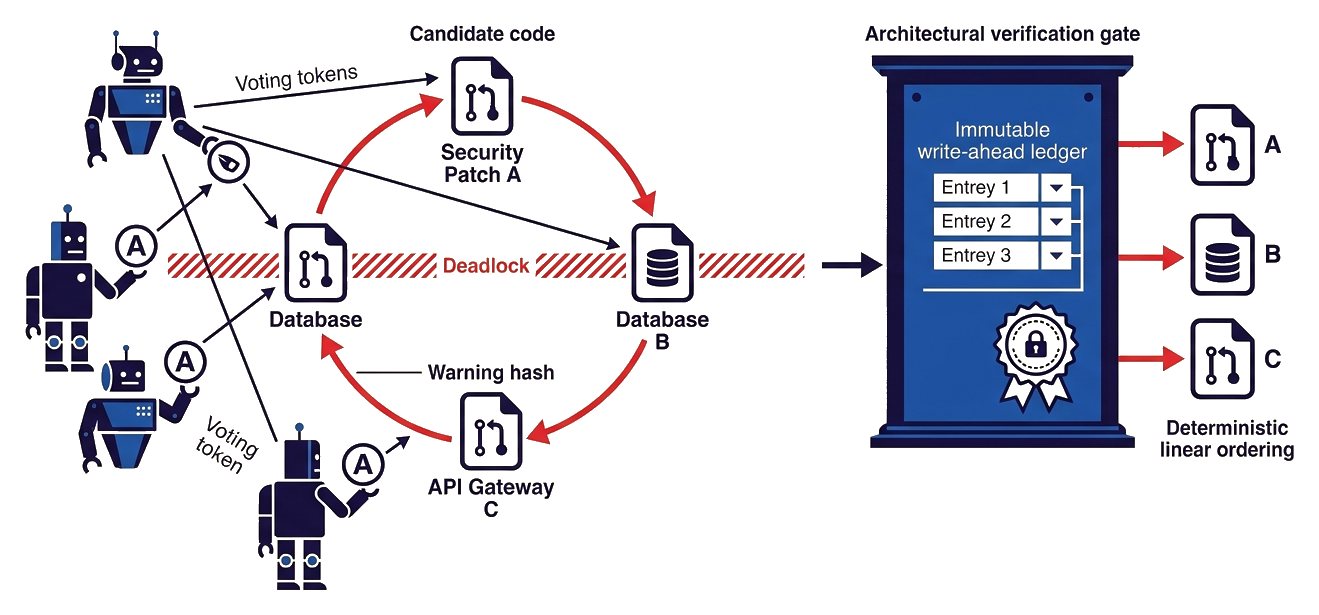
\includegraphics[width=0.88\linewidth]{figures/fig-arrows-impossibility.png}
\caption{Arrow's Impossibility Theorem across civic municipal governance and multi-agent merge queues, creating an intransitive Condorcet cycle ($PR_A \succ PR_B \succ PR_C \succ PR_A$).}
\label{fig:arrows-theorem}
\end{figure}

\begin{table}[htbp]
\centering
\fontsize{6.8}{8.5}\selectfont
\setlength{\tabcolsep}{3.5pt}
\begin{tabularx}{\linewidth}{@{}l >{\raggedright\arraybackslash}X >{\raggedright\arraybackslash}X@{}}
\toprule
\textbf{Structural Dimension} & \textbf{Civic Municipal Dilemma} & \textbf{Agent Swarm CI/CD Merge Dilemma} \\
\midrule
\textbf{Deciding Actors} & 3 City Council factions (Transit, Flood, Health) & 3 Autonomous agents ($\alpha_{\text{sec}}$, $\alpha_{\text{db}}$, $\alpha_{\text{api}}$) \\
\textbf{Competing Options} & Subway ($A$), Flood Levee ($B$), Hospital ($C$) & OpenSSL CVE ($PR_A$), Schema Mig ($PR_B$), Gateway ($PR_C$) \\
\textbf{Actor 1 Preference} & $A \succ B \succ C$ (Transit priority) & $PR_A \succ PR_B \succ PR_C$ (Zero-day vulnerability patch) \\
\textbf{Actor 2 Preference} & $B \succ C \succ A$ (Flood mitigation priority) & $PR_B \succ PR_C \succ PR_A$ (Exclusive table lock migration) \\
\textbf{Actor 3 Preference} & $C \succ A \succ B$ (Public health priority) & $PR_C \succ PR_A \succ PR_B$ (Microservice route refactor) \\
\midrule
\textbf{Pairwise Majority} & $2/3$ prefer $A \succ B$; $2/3$ prefer $B \succ C$ & $2/3$ prefer $PR_A \succ PR_B$; $2/3$ prefer $PR_B \succ PR_C$ \\
\textbf{Condorcet Cycle} & $2/3$ prefer $C \succ A \implies \mathbf{A \succ B \succ C \succ A}$ & $2/3$ prefer $PR_C \succ PR_A \implies \mathbf{PR_A \succ PR_B \succ PR_C \succ PR_A}$ \\
\textbf{Arrow's Theorem} & No fair ordinal social choice without a dictator & Democratic voting produces deadlock or agenda manipulation \\
\midrule
\textbf{Kernel Resolution} & Political compromise or centralized mandate & \textbf{Deterministic Invariant Attestation}: reject voting; \\
& & linearize via AST verification receipts and WAL commit \\
\bottomrule
\end{tabularx}
\caption{Civic voting paradoxes vs.\ agent merge deadlocks under Arrow's Theorem, resolved by deterministic kernel attestation.}
\label{tab:arrows-comparison}
\end{table}

As Figure~\ref{fig:arrows-theorem} and Table~\ref{tab:arrows-comparison} demonstrate, the structure of the civic dilemma and the multi-agent merge queue are formally identical. In both cases, ordinal ranking cannot escape the tripartite tradeoff of Arrow's Theorem: non-dictatorship, Pareto efficiency, and independence of irrelevant alternatives (IIA).

The Operating Kernel resolves this impossibility not by tuning the voting algorithm, but by \textbf{rejecting social choice voting entirely}. The kernel evaluates candidate state transitions through deterministic attestation gates ($\mathcal{V}(s, a) = \mathtt{PASS}$), AST symbol/region lease checks, and single-writer write-ahead ledger (WAL) linear commitment. When priorities conflict, order is established by monotonic dependency DAG topology and priority-fee staking (Chapter 6), never subjective agent consensus.

\subsubsection{The VCG Mechanism and Dominant-Strategy Incentive Compatibility}
In quasi-linear environments where agents have private valuations $v_i(o, \theta_i)$ and make monetary transfers $p_i$, the \textbf{Vickrey--Clarke--Groves (VCG)} mechanism aligns private incentives with global social welfare $W(o) = \sum_{i} v_i(o, \theta_i)$.

Under VCG, the mechanism determines the socially optimal outcome:
\begin{equation}
o^* \;=\; \arg\max_{o \in O} \sum_{j} v_j(o, \hat{\theta}_j)
\end{equation}
and charges each agent $i$ its Clarke pivot payment:
\begin{equation}
p_i(\hat{\theta}) \;=\; \max_{o \in O} \sum_{j \neq i} v_j(o, \hat{\theta}_j) \;-\; \sum_{j \neq i} v_j(o^*, \hat{\theta}_j)
\end{equation}
The Clarke payment equals the exact negative externality agent $i$'s presence imposes on all other participants. Under VCG, truth-telling ($\hat{\theta}_i = \theta_i$) is a strictly dominant strategy (DSIC).

\subsubsection{The Myerson--Satterthwaite Boundary}
The Myerson--Satterthwaite Theorem (1983) proves that no bilateral trade mechanism can simultaneously achieve: (1)~Dominant-strategy incentive compatibility; (2)~Ex-post Pareto efficiency; (3)~Individual rationality; and (4)~Budget balance without an external subsidy. In local agent economies (Chapter 6), resource clearing must explicitly trade off budget balance against exact allocative efficiency.

\pdmarginpagebreak

\section{Modern Coding Agent Architectures}\label{sec:prereq-coding-agents}

We now transition from classical multi-agent foundations to contemporary coding agents, examining how modern LLM-based harnesses interface with host execution environments.

\subsection{The Contemporary Landscape: Systems Comparison}

Contemporary coding agents bridge unstructured natural language reasoning with deterministic host tools (shells, AST parsers, compilers, git checkouts). Table~\ref{tab:coding-agents} compares the five leading production architectures:

\begin{table}[H]
\centering
\footnotesize
\setlength{\tabcolsep}{2.5pt}
\begin{tabularx}{\textwidth}{l >{\raggedright\arraybackslash}X >{\raggedright\arraybackslash}X >{\raggedright\arraybackslash}X >{\raggedright\arraybackslash}X}
\toprule
\textbf{Agent} & \textbf{Isolation Boundary} & \textbf{Context Strategy} & \textbf{Tool Interface} & \textbf{Rollback Engine} \\
\midrule
\textbf{Claude Code} & Subprocess + Seatbelt & Progressive disclosure & File edit, bash, MCP & Git commit checkpoint \\
\textbf{Codex CLI} & Container sandbox & History compaction & Sandboxed patch apply & Ephemeral container reset \\
\textbf{Gemini CLI} & Local / Cloud Run & 1M--2M token window & POSIX CLI, GCP SDK & Workspace rewind \\
\textbf{Aider} & Host process & Repo-map (Tree-sitter) & Git-backed diff engine & Automatic git commit undo \\
\textbf{Devin} & MicroVM (Firecracker) & Multi-buffer browser/shell & Full root pseudo-terminal & Snapshot restoration \\
\bottomrule
\end{tabularx}
\caption{Architectural comparison of contemporary production coding agents.}
\label{tab:coding-agents}
\end{table}

\subsection{Closed-Loop Deliberation vs. Open-Loop Sampling}

Stateless code generation evaluates an autoregressive distribution $Y \sim P_\theta(Y \mid X)$ in an open loop. Any syntactic, semantic, or environmental error compounds irreversibly:
\begin{equation}
\mathrm{ErrorRate}_{\text{open-loop}}(T) \;=\; 1 - \prod_{t=1}^T (1 - \epsilon_t)
\end{equation}

In contrast, an agent harness operates as a Partially Observable Markov Decision Process (POMDP):
\begin{equation}
\mathcal{M} \;=\; \langle \mathcal{S}, \mathcal{A}, \mathcal{T}, \mathcal{R}, \Omega, \mathcal{O}, \gamma \rangle
\end{equation}
where $\mathcal{S}$ is the true environment state (filesystem, git index, running processes), $\mathcal{A}$ is the action space (tool invocations), $\Omega$ is the observation space (stdout, stderr, exit codes), and $\mathcal{O}$ generates observations. The agent maintains a belief state $b_t = \mathrm{Pr}(s_t \mid h_t)$ conditioned on history $h_t = (a_0, o_0, \dots, a_{t-1}, o_{t-1})$.

\subsubsection{Deliberation Frameworks}
Four primary frameworks govern closed-loop agent reasoning:
\begin{enumerate}[leftmargin=1.8em,itemsep=2pt]
  \item \textbf{ReAct (Reasoning and Acting)~\pdcite{yao2022react}:} Interleaves natural language reasoning traces (``Thoughts'') with structured tool executions (``Actions'') and environment feedback (``Observations''). When factual uncertainty is encountered, reasoning halts and an exploratory tool is invoked.
  \item \textbf{Tree of Thoughts (ToT)~\pdcite{yao2023tree}:} Explores search trees over candidate thought steps using BFS, DFS, or MCTS, evaluating intermediate node viability via self-critique rubrics and backtracking upon failure.
  \item \textbf{Reflexion~\pdcite{shinn2023reflexion}:} Employs verbal reinforcement learning. Upon task failure, the model generates linguistic self-reflections that are stored in an episodic memory buffer and prepended to subsequent execution prompts.
  \item \textbf{Plan-and-Solve:} Divides execution into a macro-planning phase (generating ordered subgoals) followed by iterative sub-task execution with explicit replanning interrupts.
\end{enumerate}

\subsection{Cognitive Control, Training, and Fine-Tuning}\label{sec:prereq-cognitive-control}

Coding agents are trained across a three-stage continuum:
\begin{enumerate}[leftmargin=1.8em,itemsep=2pt]
  \item \textbf{Pre-Training:} Self-supervised next-token autoregressive modeling over trillions of tokens of source code, version history, documentation, and technical literature:
  \begin{equation}
  \mathcal{L}_{\mathrm{PT}}(\theta) \;=\; -\mathbb{E}_{x \sim \mathcal{D}}\left[ \sum_t \log P_\theta(x_t \mid x_{<t}) \right]
  \end{equation}
  \item \textbf{Tool-Use Supervised Fine-Tuning (SFT):} Training over multi-turn trajectories with \emph{loss masking}: loss gradients are computed strictly over model-generated tool calls and arguments, masking prompt context and tool output tokens.
  \item \textbf{Reinforcement Learning Alignment (RLHF / DPO):} Direct Preference Optimization optimizes policy weights over paired trajectories without training an explicit reward model:
  \begin{align}
  \mathcal{L}_{\mathrm{DPO}}(\theta; \theta_{\mathrm{ref}}) \;&=\; -\mathbb{E}_{(x, y_w, y_l)}\Big[ \log \sigma \Big( \beta \log \frac{\pi_\theta(y_w \mid x)}{\pi_{\mathrm{ref}}(y_w \mid x)} \nonumber \\
  &\qquad\qquad\qquad\quad -\; \beta \log \frac{\pi_\theta(y_l \mid x)}{\pi_{\mathrm{ref}}(y_l \mid x)} \Big) \Big]
  \end{align}
\end{enumerate}

\subsubsection{Test-Time Compute and Process Reward Models}
Reasoning-focused frontier models shift compute to inference time. Instead of sampling greedily, inference search trees explore alternative reasoning chains scored by \textbf{Process Reward Models (PRMs)} that evaluate correctness at each logical derivation step:
\begin{equation}
\mathrm{Score}(\tau) \;=\; \prod_{t=1}^T \mathrm{PRM}(c_t \mid c_{<t}, x)
\end{equation}
When an intermediate verification score falls below a threshold $\tau_{\mathrm{cut}}$, the search beam backtracks to a previous checkpoint.

\subsection{Instruction Hierarchy and Context Economics}\label{sec:prereq-transformers}

A fundamental vulnerability of LLM architectures is the absence of hardware-enforced privilege separation between instructions and data. An agent that reads an untrusted file or issue comment is susceptible to \textbf{indirect prompt injection}, where malicious text commandeers model control flow. Production harnesses enforce strict instruction hierarchies: system prompts occupy privileged framing, while user inputs and tool outputs are quarantined in escaped delimitations.

\subsubsection{The KV-Cache Asymptotics}
During autoregressive decoding, key and value activations for preceding tokens are stored in high-bandwidth memory (HBM). For a model with $L$ layers, $N_h$ KV-heads, dimension $d_h$, and precision bytes $b_p$, the memory footprint for a context of length $T$ is:
\begin{equation}\label{eq:kv-cache-mem}
\mathrm{Memory}_{\mathrm{KV}} \;=\; 2 \times L \times N_h \times d_h \times T \times b_p \quad \text{bytes}
\end{equation}
For a 70-billion parameter model ($L=80, N_h=8, d_h=128, b_p=2$), each context token consumes $\approx 320\text{ KB}$. At $T = 128{,}000$ tokens, the KV-cache consumes $\approx 40.96\text{ GB}$ of VRAM per concurrent agent.

\begin{pdexample}{Numbers by hand: KV-cache memory exhaustion}
\setlength{\parskip}{4pt plus 1pt}
Calculate the physical high-bandwidth memory (HBM) required to support a small fleet of concurrent coding subagents. Suppose we deploy an 8-agent specialized swarm (1~orchestrator, 4~domain coders, 1~test harness runner, 1~adversarial reviewer, and 1~docs compiler) backed by a 70-billion parameter frontier dense model with $L = 80$ transformer layers, grouped-query attention using $N_h = 8$ key-value head pairs, per-head dimension $d_h = 128$, and 16-bit floating point precision ($b_p = 2$ bytes).

First, price the KV memory footprint of a single token using Eq.~\eqref{eq:kv-cache-mem}:
\[
\mathrm{Memory}_{\mathrm{token}} \;=\; 2 \times 80 \times 8 \times 128 \times 2 \;=\; 327{,}680\text{ bytes} \;\approx\; 320\text{ KiB}.
\]
When each agent works across an active multi-turn session of length $T = 128{,}000$ tokens (reading AST symbol maps, terminal outputs, and compiler diagnostics), each agent's active cache footprint reaches:
\[
\mathrm{Memory}_{\mathrm{KV}}(T) \;=\; 128{,}000 \times 327{,}680\text{ bytes} \;\approx\; 41.94\text{ GB}.
\]
For our 8-agent fleet, the concurrent KV-cache alone demands:
\[
8 \times 41.94\text{ GB} \;=\; 335.54\text{ GB of HBM3}.
\]
Before reserving a single byte for the base model weights ($70\text{B} \times 2\text{ bytes} \approx 140\text{ GB}$), the agent fleet requires five 80~GB H100 GPUs exclusively dedicated to storing historical tokens. If an agent attempts to maintain state by dumping verbose JSON test traces directly into its prompt context, it induces rapid memory exhaustion, forcing the inference scheduler to page activations to host DDR memory (spiking generation latency by $\sim 25\times$) or evict tokens, inducing disastrous task amnesia. Durable coordination state must therefore be externalized into an out-of-band kernel ledger.
\end{pdexample}

\begin{pdclaim}{Theorem}{The Ephemeral Memory Limit}\label{thm:ephemeral-memory}
The context window of a transformer is volatile, expensive, and subject to attention dilution (effective information retrieval degrades with sequence depth~\cite{liu2024lost}). Consequently, long-term system state cannot be maintained by continuously appending tool execution logs to the prompt. Durable state must reside in an external, indexed, and ACID-compliant storage engine.
\end{pdclaim}

\section{Tools, Protocols, Skills, and Hooks}\label{sec:prereq-hypervisors}

To interact safely with the host environment, an agent harness must govern tool dispatch, encapsulate domain knowledge, and enforce runtime invariants.

\subsection{Tool Dispatch and the Model Context Protocol (MCP)}

The Model Context Protocol (MCP) standardizes agent-to-tool communication using JSON-RPC 2.0. MCP defines four core primitives:
\begin{itemize}[leftmargin=1.8em,itemsep=2pt]
  \item \textbf{Tools:} Executable actions with strict JSON-Schema input validation and structured result payloads.
  \item \textbf{Resources:} URI-addressable read-only context (files, database rows, logs).
  \item \textbf{Prompts:} Parametric prompt templates engineered for specific operational workflows.
  \item \textbf{Sampling:} Protocol affordances enabling servers to request nested LLM inference through the client harness under client permission boundaries.
\end{itemize}

\subsection{Skill Architectures and Progressive Disclosure}

A critical architectural challenge in agent design is \emph{context bloat}. Injecting complete documentation, code examples, and reference manuals for hundreds of specialized tools into the agent's system prompt exhausts context limits and induces severe attention dilution~\cite{liu2024lost}. If an agent repository maintains 500 specialized domain skills, each averaging 10,000 tokens of documentation, monolithic injection would require $5{,}000{,}000$ tokens per inference turn---exceeding the physical memory capacity of frontier models and incurring catastrophic monetary and latency costs.

Modern agent harnesses resolve this dilemma via \textbf{Three-Tier Progressive Disclosure} (Figure~\ref{fig:progressive-skills-iceberg}):
\begin{enumerate}[leftmargin=1.8em,itemsep=3pt]
  \item \textbf{Tier 1 (Surface Frontmatter Index):} The system prompt contains only lightweight index entries: the skill's unique identifier and a concise 1-to-2 sentence description ($10^1$--$10^2$ tokens per skill). Across a library of 500 skills, this consumes a static footprint of $\approx 15{,}000$ tokens ($\approx 7.5\%$ of a 200k context window). Because Tier~1 is static across all turns, modern inference providers cache this prompt prefix in HBM, reducing input costs by up to $90\%$. The probability of inclusion in the prompt is $P = 1.0$.
  \item \textbf{Tier 2 (On-Demand Instruction Activation):} When the agent's semantic classifier or planning policy determines that a task requires a specific capability, it invokes a read tool to load the corresponding \path{SKILL.md} into its working context ($10^3$--$10^4$ tokens). Tier~2 contains operational instructions, parameter constraints, decision tables, and error recovery protocols. Its activation probability is conditionally sparse ($P \approx 10^{-1}$), loaded only for the duration of the subtask and purged or compacted when the goal is achieved.
  \item \textbf{Tier 3 (Deep Reference and Subprocess Execution):} Beneath the instruction manual lies the deepest architectural layer: specialized executable scripts (\path{scripts/}), schemas, and large reference manuals (\path{references/}), spanning $10^4$--$10^5$ tokens. Crucially, the agent \emph{does not load Tier~3 assets into its language context}. Instead, Tier~2 instructs the agent to execute Tier~3 scripts in an isolated host subshell or query specific byte offsets on demand. Because invoking a specialized script or deep reference is needed only for esoteric domain edge-cases, its execution probability is orders of magnitude lower ($P \approx 10^{-3}$ to $10^{-4}$).
\end{enumerate}

\providecolor{pdcyan}{HTML}{00859B}
\begin{figure}[htbp]
\centering
\begin{tikzpicture}[pd figure,x=1cm,y=1cm]
  \useasboundingbox (0, 0.4) rectangle (11.4, 7.2);
  
  % 1. Logarithmic Graph Paper Background (4 Decades: 10^-4 to 10^0) across 11.4cm
  \draw[draw=pdcyan!35,fill=pdcyan!3,line width=0.6pt] (1.2, 0.5) rectangle (11.2, 6.9);
  
  % Vertical grid lines across graph paper
  \foreach \gx in {2.2, 3.2, 4.2, 5.2, 6.2, 7.2, 8.2, 9.2, 10.2} {
    \draw[draw=pdcyan!14,line width=0.2pt] (\gx, 0.5) -- (\gx, 6.9);
  }
  
  % Horizontal log sub-grid lines within each decade (height = 1.55cm per decade)
  % Decade 0: 10^-4 to 10^-3 (y: 0.6 to 2.15)
  % Decade 1: 10^-3 to 10^-2 (y: 2.15 to 3.70)
  % Decade 2: 10^-2 to 10^-1 (y: 3.70 to 5.25)
  % Decade 3: 10^-1 to 10^0  (y: 5.25 to 6.80)
  \foreach \dec in {0, 1, 2, 3} {
    \foreach \sub in {2, 3, 4, 5, 6, 7, 8, 9} {
      \pgfmathsetmacro{\suby}{0.6 + \dec*1.55 + 1.55*log10(\sub)}
      \draw[draw=pdcyan!18,line width=0.2pt] (1.2, \suby) -- (11.2, \suby);
    }
    \pgfmathsetmacro{\decy}{0.6 + \dec*1.55}
    \draw[draw=pdcyan!50,line width=0.6pt] (1.2, \decy) -- (11.2, \decy);
  }
  \draw[draw=pdcyan!50,line width=0.6pt] (1.2, 6.8) -- (11.2, 6.8);

  % Y-Axis Ticks and Logarithmic Labels
  \node[anchor=east,font=\fontsize{6.0}{7.0}\selectfont\bfseries] at (1.15, 6.8) {$10^0$};
  \node[anchor=east,font=\fontsize{4.8}{5.8}\selectfont\color{pdinkmuted}] at (1.15, 6.55) {100\%};

  \node[anchor=east,font=\fontsize{6.0}{7.0}\selectfont\bfseries] at (1.15, 5.25) {$10^{-1}$};
  \node[anchor=east,font=\fontsize{4.8}{5.8}\selectfont\color{pdinkmuted}] at (1.15, 5.0) {10\%};

  \node[anchor=east,font=\fontsize{6.0}{7.0}\selectfont\bfseries] at (1.15, 3.70) {$10^{-2}$};
  \node[anchor=east,font=\fontsize{4.8}{5.8}\selectfont\color{pdinkmuted}] at (1.15, 3.45) {1\%};

  \node[anchor=east,font=\fontsize{6.0}{7.0}\selectfont\bfseries] at (1.15, 2.15) {$10^{-3}$};
  \node[anchor=east,font=\fontsize{4.8}{5.8}\selectfont\color{pdinkmuted}] at (1.15, 1.90) {0.1\%};

  \node[anchor=east,font=\fontsize{6.0}{7.0}\selectfont\bfseries] at (1.15, 0.60) {$10^{-4}$};
  \node[anchor=east,font=\fontsize{4.8}{5.8}\selectfont\color{pdinkmuted}] at (1.15, 0.40) {0.01\%};

  \node[anchor=center,rotate=90,font=\fontsize{5.2}{6.2}\selectfont\color{pdcobalt}\bfseries] at (0.35, 3.7) {ACTIVATION PROBABILITY $P(\text{task})$ PER TURN (LOG SCALE)};

  % Prompt Waterline (boundary between prompt injection and on-disk files)
  \draw[draw=pdcobalt,line width=1.1pt,dashed] (1.2, 5.26) -- (11.2, 5.26);
  \node[anchor=center, font=\fontsize{4.8}{5.8}\selectfont\color{pdcobalt}\bfseries, fill=white, inner sep=1.5pt] at (6.2, 5.26) {PROMPT WATERLINE (IN-CONTEXT) $\blacktriangledown$ \quad {\color{pdinkmuted}\textperiodcentered \quad $\blacktriangle$ ON-DISK REPOSITORY (SUBPROCESS)}};

  % Logarithmic Decay Sparkline Curve
  \draw[draw=pdcobalt!85,line width=1.8pt,-{Stealth[length=5pt,width=3.5pt]}]
    (2.5, 6.25) .. controls (3.8, 5.8) and (4.2, 4.4) ..
    (5.2, 3.65) .. controls (6.2, 2.9) and (7.0, 1.7) .. (10.0, 1.15);
  \node[anchor=south west,font=\fontsize{4.8}{5.8}\selectfont\bfseries\color{pdcobalt},fill=white,fill opacity=0.9,inner sep=1.2pt]
    at (4.4, 4.25) {Log Decay Sparkline: Context Consumption $\propto \log(P)$};

  % TIER 1: YAML Frontmatter Header (P = 1.0)
  \draw[draw=pdcobalt,fill=white,fill opacity=0.96,line width=0.8pt,rounded corners=2pt] (2.7, 5.85) rectangle (9.9, 6.65);
  \node[anchor=west,font=\fontsize{5.6}{6.6}\selectfont\color{pdcobalt}\bfseries] at (2.9, 6.40) {TIER 1: YAML FRONTMATTER INDEX};
  \node[anchor=east,font=\fontsize{5.0}{6.0}\selectfont\ttfamily\color{pdink}] at (9.7, 6.40) {SKILL.md};
  \node[anchor=west,font=\fontsize{4.8}{5.8}\selectfont\color{pdink}] at (2.9, 6.08) {$P = 1.0$ (Every Turn) $\;\cdot\;$ $\approx 30$ tok/skill $\;\cdot\;$ \textbf{HBM Prefix Cached}};

  % TIER 2: SKILL.md Markdown Body (P ~ 10^-1)
  \draw[draw=pdindigo,fill=white,fill opacity=0.96,line width=0.8pt,rounded corners=2pt] (2.7, 4.45) rectangle (9.9, 5.20);
  \node[anchor=west,font=\fontsize{5.6}{6.6}\selectfont\color{pdindigo}\bfseries] at (2.9, 4.97) {TIER 2: ON-DEMAND INSTRUCTION MANUAL};
  \node[anchor=east,font=\fontsize{5.0}{6.0}\selectfont\ttfamily\color{pdink}] at (9.7, 4.97) {SKILL.md Body};
  \node[anchor=west,font=\fontsize{4.8}{5.8}\selectfont\color{pdink}] at (2.9, 4.67) {$P \approx 10^{-1}$ (On-Demand) $\;\cdot\;$ $2\text{k}$--$5\text{k}$ tok/task $\;\cdot\;$ \textbf{Active Working Context}};

  % TIER 2.5: Subagents & References (P ~ 10^-2)
  \draw[draw=pdviolet!80,fill=white,fill opacity=0.96,line width=0.8pt,rounded corners=2pt] (2.7, 2.95) rectangle (9.9, 3.70);
  \node[anchor=west,font=\fontsize{5.6}{6.6}\selectfont\color{pdviolet!90}\bfseries] at (2.9, 3.47) {TIER 2.5: SPECIALIZED SUBAGENTS \& REFERENCES};
  \node[anchor=east,font=\fontsize{5.0}{6.0}\selectfont\ttfamily\color{pdink}] at (9.7, 3.47) {agents/ \& refs/};
  \node[anchor=west,font=\fontsize{4.8}{5.8}\selectfont\color{pdink}] at (2.9, 3.17) {$P \approx 10^{-2}$ (Spawn/Lookup) $\;\cdot\;$ $10\text{k}$--$30\text{k}$ tok/delegate $\;\cdot\;$ \textbf{Isolated Subagent}};

  % TIER 3: Executables & Schemas (P ~ 10^-3 to 10^-4)
  \draw[draw=pdink!80,fill=white,fill opacity=0.96,line width=0.8pt,rounded corners=2pt] (2.7, 1.35) rectangle (9.9, 2.10);
  \node[anchor=west,font=\fontsize{5.6}{6.6}\selectfont\color{pdink}\bfseries] at (2.9, 1.87) {TIER 3: HOST EXECUTABLES \& FORMAL SCHEMAS};
  \node[anchor=east,font=\fontsize{5.0}{6.0}\selectfont\ttfamily\color{pdink}] at (9.7, 1.87) {scripts/ \& schemas/};
  \node[anchor=west,font=\fontsize{4.8}{5.8}\selectfont\color{pdink}] at (2.9, 1.57) {$P \approx 10^{-3}$--$10^{-4}$ (Subprocess) $\;\cdot\;$ \textbf{\color{pdhealth}0 TOKENS IN CONTEXT} $\;\cdot\;$ \textbf{Native Sandbox}};
\end{tikzpicture}
\caption{The Progressive Disclosure of Skills drafted across logarithmic graph paper. By partitioning capabilities across four decades of activation frequency---from baseline YAML frontmatter ($P=1.0$), through on-demand \texttt{SKILL.md} manuals ($P \approx 10^{-1}$) and specialized \texttt{agents/} and \texttt{references/} ($P \approx 10^{-2}$), down to host-executed \texttt{scripts/} and \texttt{schemas/} ($P \approx 10^{-3}$--$10^{-4}$) consuming zero LLM context tokens---the log curve acts as a visual sparkline showing how context consumption contracts exponentially with task specialization.}
\label{fig:progressive-skills-iceberg}
\end{figure}

\subsection{Lifecycle Hooks and Supervisory Control}

Harness lifecycle hooks intercept agent control flow at critical execution boundaries. Formally, lifecycle hooks operate as a \textbf{Ramadge--Wonham Supervisory Controller} ($S / G$).

Let the unconstrained agent execution be modeled as a discrete-event generator $G = \langle X, \Sigma, \delta, x_0, X_m \rangle$, where events $\Sigma = \Sigma_c \cup \Sigma_u$ are partitioned into controllable events $\Sigma_c$ (tool invocations, file writes, network requests) and uncontrollable events $\Sigma_u$ (model token generation, host hardware interrupts, external process termination). A supervisory hook $S: L(G) \to \mathcal{P}(\Sigma)$ dynamically disables tool invocations that violate safety invariants:
\begin{equation}
L(S / G) \;\subseteq\; K \;\subset\; L(G)
\end{equation}
where $K$ is the formal language of safe execution traces (e.g., preventing writes to protected branches, restricting filesystem mutations to leased workspaces, or halting when spending caps are exceeded).

Figure~\ref{fig:lifecycle-hooks-engines} formalizes the complete cross-section of modern production agent lifecycle hooks, modeled after the production architecture of Anthropic's Claude Code and the Port Daddy Giant Squid Harness. Execution proceeds through two nested supervisory loops:
\begin{enumerate}[leftmargin=1.8em,itemsep=2pt]
  \item \textbf{The Outer Session \& Turn Loop:} Encompasses initial context injection (\texttt{SessionStart}), prompt interception (\texttt{UserPromptSubmit}), context pressure management (\texttt{PreCompact}), turn-level invariant verification (\texttt{Stop}/\texttt{StopFailure}), and session teardown (\texttt{SessionEnd}).
  \item \textbf{The Inner Agentic Tool Loop:} Governs the iterative reasoning-action cycle: pre-tool interception and deterministic vetoes (\texttt{PreToolUse}), sandboxed execution, and reactive post-tool sanitization (\texttt{PostToolUse}).
\end{enumerate}

\begin{figure}[htbp]
\centering
\begin{tikzpicture}[pd figure,x=1cm,y=1cm,
  hk start/.style={draw=pdhealth!80,fill=pdhealth!12,line width=0.8pt,rounded corners=2pt,align=center,font=\fontsize{5.6}{6.6}\selectfont\color{pdhealth}\bfseries},
  hk core/.style={draw=pdcobalt!80,fill=pdcobalt!8,line width=0.8pt,rounded corners=2pt,align=center,font=\fontsize{5.6}{6.6}\selectfont\color{pdcobalt}\bfseries},
  hk stop/.style={draw=pderror!80,fill=pderror!12,line width=0.8pt,rounded corners=2pt,align=center,font=\fontsize{5.6}{6.6}\selectfont\color{pderror}\bfseries},
  hk compact/.style={draw=pdviolet!80,fill=pdviolet!10,line width=0.8pt,rounded corners=2pt,align=center,font=\fontsize{5.6}{6.6}\selectfont\color{pdviolet!90}\bfseries},
  hk llm/.style={draw=pdgold!90,fill=pdgold!15,line width=0.9pt,rounded corners=2pt,align=center,font=\fontsize{5.8}{6.8}\selectfont\color{pdink}\bfseries},
  hk gate/.style={draw=pdcobalt,fill=white,line width=0.9pt,rounded corners=2pt,align=center,font=\fontsize{5.6}{6.6}\selectfont\color{pdcobalt}\bfseries},
  hk sandbox/.style={draw=pdink!80,fill=pdink!6,line width=0.8pt,rounded corners=2pt,align=center,font=\fontsize{5.6}{6.6}\selectfont\color{pdink}\bfseries},
  hk post/.style={draw=pdindigo,fill=pdindigo!10,line width=0.8pt,rounded corners=2pt,align=center,font=\fontsize{5.6}{6.6}\selectfont\color{pdindigo}\bfseries},
  hk edge/.style={draw=pdink!80,line width=0.7pt,-{Stealth[length=4pt,width=3pt]}},
  hk allow edge/.style={draw=pdhealth!90,line width=0.9pt,-{Stealth[length=4pt,width=3pt]}},
  hk deny edge/.style={draw=pderror!90,line width=0.9pt,-{Stealth[length=4pt,width=3pt]}},
  hk loop edge/.style={draw=pdcobalt,line width=0.8pt,-{Stealth[length=4pt,width=3pt]}}
]
  \useasboundingbox (0, 0) rectangle (11.4, 9.6);

  % =========================================================================
  % CONTAINER 1: Outer Session & Turn Loop (Left Column: x: 0.1 to 4.7)
  % =========================================================================
  \draw[draw=pdcobalt!40,fill=pdcobalt!2,rounded corners=3pt,line width=0.6pt] (0.1, 0.65) rectangle (4.7, 9.45);
  \node[anchor=north,font=\fontsize{6.2}{7.2}\selectfont\color{pdcobalt}\bfseries] at (2.40, 9.30) {OUTER SESSION \& TURN LIFECYCLE};

  \node[hk start,text width=3.8cm] (start) at (2.40, 8.40) {
    \textbf{SessionStart: Context Ingress}\\[1pt]
    {\fontsize{4.8}{5.8}\selectfont\normalfont Injects branch, active locks, inbox}
  };

  \node[hk core,text width=3.8cm] (prompt) at (2.40, 6.95) {
    \textbf{UserPromptSubmit: Turn Ingress}\\[1pt]
    {\fontsize{4.8}{5.8}\selectfont\normalfont Prompt normalization $\cdot$ Worktree lease}
  };
  \draw[hk edge] (start) -- (prompt);

  \node[hk stop,text width=3.8cm] (stop) at (2.40, 4.45) {
    \textbf{Stop / StopFailure: Test Gate}\\[1pt]
    {\fontsize{4.8}{5.8}\selectfont\normalfont Verification suite $\cdot$ Exit 0 vs Exit 2}
  };

  \node[hk compact,text width=3.8cm] (precomp) at (2.40, 2.75) {
    \textbf{PreCompact: Memory Snapshot}\\[1pt]
    {\fontsize{4.8}{5.8}\selectfont\normalfont At $85\%$ tokens: dump plan to disk}
  };
  \draw[hk edge] (stop) -- (precomp);

  \node[hk core,text width=3.8cm] (send) at (2.40, 1.25) {
    \textbf{SessionEnd: Clean Teardown}\\[1pt]
    {\fontsize{4.8}{5.8}\selectfont\normalfont Release locks $\cdot$ Graveyard salvage}
  };
  \draw[hk edge] (precomp) -- (send);

  % =========================================================================
  % CONTAINER 2: Inner Agentic Tool Loop (Right Column: x: 5.1 to 11.3)
  % =========================================================================
  \draw[draw=pdgold!90,line width=0.8pt,rounded corners=3pt,fill=pdgold!4] (5.1, 0.65) rectangle (11.3, 9.45);
  \node[anchor=north,font=\fontsize{6.2}{7.2}\selectfont\color{pdgold!90}\bfseries] at (8.20, 9.30) {INNER AGENTIC REASONING \& TOOL LOOP};

  \node[hk llm,text width=5.2cm] (agent_delib) at (8.20, 8.40) {
    \textbf{Agent Deliberation: Policy $\pi_\theta(a_t \mid C_t)$}\\[1pt]
    {\fontsize{4.8}{5.8}\selectfont\normalfont Proposes tool call $a_t$ or final answer}
  };

  \node[hk gate,text width=5.2cm] (pretool) at (8.20, 6.70) {
    \textbf{PreToolUse: Interception Gate}\\[1pt]
    {\fontsize{4.8}{5.8}\selectfont\normalfont Pattern match: \texttt{Bash | Edit | Write | Spawn}}
  };
  \draw[hk edge] (agent_delib) -- (pretool);

  % Decision branch: Exit 2 (VETO) loops back on right side
  \draw[hk deny edge] (pretool.east) -- (11.0, 6.70) -- (11.0, 8.40) -- (agent_delib.east);
  \node[anchor=west,font=\fontsize{4.8}{5.8}\selectfont\color{pderror}\bfseries,align=left] at (10.35, 7.55) {Exit 2\\Veto};

  \node[hk sandbox,text width=5.2cm] (sandbox) at (8.20, 4.85) {
    \textbf{[Seatbelt Sandbox Confinement]}\\[1pt]
    {\fontsize{4.8}{5.8}\selectfont\normalfont Isolated worktree $\cdot$ Metered network egress}
  };
  \draw[hk allow edge] (pretool) -- (sandbox)
    node[midway,right=2pt,font=\fontsize{4.8}{5.8}\selectfont\color{pdhealth}\bfseries] {Exit 0 (Allow)};

  \node[hk post,text width=5.2cm] (posttool) at (8.20, 3.00) {
    \textbf{PostToolUse: Hygiene \& Secret Scrubbing}\\[1pt]
    {\fontsize{4.8}{5.8}\selectfont\normalfont AST format (\texttt{biome}) $\cdot$ Redact credentials}
  };
  \draw[hk edge] (sandbox) -- (posttool);

  % Loopback from PostToolUse back to Agent Deliberation
  \draw[hk loop edge] (posttool.west) -- (5.45, 3.00) -- (5.45, 8.40) -- (agent_delib.west);
  \node[anchor=east,font=\fontsize{4.8}{5.8}\selectfont\color{pdcobalt}\bfseries,align=right] at (5.45, 5.70) {Next turn\\$\mathcal{O}_{t+1}$};

  % Cross-Loop Edges:
  % Prompt to Agent Deliberation
  \draw[hk edge] (prompt.east) -- (agent_delib.south west);

  % Agent done -> Stop Gate
  \draw[hk edge] (agent_delib.south west) -- (stop.north east)
    node[midway,above=2pt,font=\fontsize{4.8}{5.8}\selectfont\color{pderror}\bfseries] {done};

  % Stop Gate Veto loopback to Agent Deliberation
  \draw[hk deny edge] (stop.east) -- (6.0, 4.45) -- (6.0, 7.80) -- (agent_delib.south);
  \node[anchor=south west,font=\fontsize{4.8}{5.8}\selectfont\color{pderror}\bfseries] at (6.0, 5.20) {Exit 2 (Test Fail)};

  % =========================================================================
  % Bottom Invariant Banner
  % =========================================================================
  \draw[draw=pdink!30,fill=pdink!3,rounded corners=2pt] (0.1, 0.05) rectangle (11.3, 0.50);
  \node[anchor=center,font=\fontsize{4.8}{5.8}\selectfont\color{pdinkmuted},text width=10.9cm,align=center] at (5.7, 0.27) {
    \textbf{Supervisory Control Invariant ($S/G$):} Deterministic hooks govern external execution ($\Sigma_c$) via binary vetoes (\texttt{Exit 0} vs \texttt{Exit 2}) and context injection, operating strictly outside the statistical model's weights.
  };
\end{tikzpicture}
\caption{The Agent Lifecycle Hook cross-section, modeled after the production architecture of Anthropic's Claude Code and the Port Daddy Giant Squid Harness. Execution is partitioned into two nested supervisory loops: the outer Session and Turn lifecycle manages user context, memory compaction (\texttt{PreCompact}), and test verification (\texttt{Stop}), while the inner \texttt{AGENTIC TOOL LOOP} supervises iterative tool invocations, pre-execution security vetoes (\texttt{PreToolUse}), sandbox execution, and reactive post-tool sanitization (\texttt{PostToolUse}).}
\label{fig:lifecycle-hooks-engines}
\end{figure}

\subsubsection{Case Studies in Lifecycle Hook Enforcement}
\label{sec:lifecycle-hook-cases}

In production harnesses, lifecycle hooks replace conversational model instructions with deterministic binary gates. The following three scenarios illustrate how the inner and outer supervisory loops enforce system invariants:

\begin{description}[leftmargin=1.5em,style=sameline,font=\normalfont]
\item[\textbf{Case A (Pre-Tool Security Veto):}] \emph{Destructive Command Interception.}
When an agent attempts a forbidden operation such as \texttt{Bash("git push -f origin main")}, the \texttt{PreToolUse} hook pattern-matches against \texttt{push.*(-f|--force)}. The hook exits with code \texttt{2} (\textbf{BLOCKED}), aborting execution before any host system call occurs. The hook injects standard-error feedback (\texttt{"VETO: force-push forbidden. Use topic branch."}) directly into the agent's observation buffer, compelling self-correction with zero physical blast radius.

\item[\textbf{Case B (Post-Tool Code Hygiene):}] \emph{Reactive Normalization and Linting.}
When an agent edits a source file via \texttt{Edit("src/auth/jwt.ts", diff)}, the \texttt{PostToolUse} hook triggers automatically on file closure. The hook executes \texttt{npx biome format --write} within the confined worktree, normalizing AST whitespace and fixing lint violations before mutations are staged or witnessed by the compiler.

\item[\textbf{Case C (Closeout Test Verification):}] \emph{Deterministic Turn Completion Gate.}
When an agent declares completion (\texttt{"I have completed the JWT refactoring"}), the \texttt{Stop} hook halts the turn and executes the unit test suite (\texttt{vitest run auth}). If any test fails, the hook exits with code \texttt{2} (\textbf{REJECTED}), preventing session exit and injecting failure diagnostics (\texttt{"Stop vetoed: test 'jwt\_verify' failed. Fix it."}). The agent cannot leave broken code in the worktree.
\end{description}

\subsubsection{What Lifecycle Hooks Allow and What They Exclude}
Understanding the mathematical boundary of lifecycle hooks is crucial for operating kernel design:
\begin{itemize}[leftmargin=1.8em,itemsep=2pt]
  \item \textbf{What Hooks Allow:}
  \begin{enumerate}[label=(\alph*),itemsep=1pt]
    \item \emph{Deterministic Pre-Execution Veto:} The \texttt{PreToolCall} hook can inspect parameters, evaluate capability macaroons, verify file leases, and abort execution before any physical syscall occurs.
    \item \emph{Parameter Normalization and Containment:} Hooks can rewrite paths to confine edits within a designated sandbox, enforcing confinement at the API boundary.
    \item \emph{Confidentiality Scrubbing:} The \texttt{PostToolCall} hook can intercept stdout/stderr, scrubbing discovered API tokens and private credentials before they enter the model's KV-cache.
    \item \emph{Spend and Time Metering:} Hooks enforce hard stopping conditions on cumulative token usage and execution time.
  \end{enumerate}
  \item \textbf{What Hooks Cannot Allow (The Inherent Limitations):}
  \begin{enumerate}[label=(\alph*),itemsep=1pt]
    \item \emph{Zero Control Over Internal Deliberation:} Hooks intercept only external events ($\Sigma_c$). They cannot steer the internal attention weights of the transformer during autoregressive generation.
    \item \emph{Cannot Repair Corrupted KV-Activations:} Once an untrusted string or misleading prompt injection enters the context buffer, hooks cannot selectively excise its semantic influence without rolling back the entire context window.
    \item \emph{Post-Hoc Ineffectiveness:} Intercepting an event after execution (\texttt{PostToolCall}) cannot undo destructive side effects (such as an unauthenticated network egress or an unbacked drop of a production table) that already occurred in the host environment.
  \end{enumerate}
\end{itemize}

\pdmarginpagebreak

\section{Multi-Agent Swarm Topologies and Interaction Patterns}\label{sec:prereq-swarms}

When multiple agents collaborate on a codebase, their interaction follows standard topological patterns:

\begin{table}[H]
\centering
\small
\begin{tabularx}{\textwidth}{l >{\raggedright\arraybackslash}X}
\toprule
\textbf{Topology} & \textbf{Coordination Characteristics} \\
\midrule
\textbf{Hierarchical Orchestrator} & A primary agent decomposes goals, spawns specialized subagents, aggregates findings, and enforces review gates. Single point of failure; prone to orchestrator context saturation. \\
\addlinespace[3pt]
\textbf{Peer-to-Peer Gossip} & Agents communicate directly via broadcast or targeted channels. Highly resilient, but vulnerable to message explosion ($O(N^2)$) and consensus divergence. \\
\addlinespace[3pt]
\textbf{Tuple Space (Blackboard)} & Agents coordinate asynchronously through an associative shared memory (Linda model). Writes, reads, and takes are atomic; enables loose temporal and spatial coupling. \\
\addlinespace[3pt]
\textbf{Market-Based Clearing} & Tasks and resources are allocated through sealed-bid or English auctions under budget constraints. Prevents resource hoarding and aligns allocation with task priority. \\
\bottomrule
\end{tabularx}
\caption{Taxonomy of multi-agent swarm interaction topologies.}
\label{tab:swarm-topologies}
\end{table}

Figure~\ref{fig:swarm-topologies-detailed} contrasts these five communication patterns geometrically, highlighting the structural failure modes of peer chatter versus the resilience of kernel-mediated stigmergy.

\begin{figure}[p]
\centering
\begin{tikzpicture}[pd figure,x=1cm,y=1cm,
  pd panel/.style={draw=pdink!25,line width=0.6pt,fill=white,rounded corners=2pt},
  pd titlebar/.style={fill=pdindigo!8,draw=pdink!20,line width=0.5pt},
  pd agent/.style={draw=pdindigo,line width=0.7pt,fill=pdindigo!10,rounded corners=2pt,align=center,font=\fontsize{5.2}{6.2}\selectfont\bfseries,inner sep=2.5pt},
  pd lead/.style={draw=pdcobalt,line width=0.9pt,fill=pdcobalt!15,rounded corners=2pt,align=center,font=\fontsize{5.6}{6.6}\selectfont\bfseries,inner sep=2.5pt},
  pd kernel/.style={draw=pdcobalt,line width=1.1pt,fill=pdcobalt!12,rounded corners=2pt,align=center,font=\fontsize{6.0}{7.0}\selectfont\bfseries,inner sep=3.5pt},
  pd task/.style={draw=pdink!70,line width=0.6pt,fill=white,rounded corners=2pt,align=center,font=\fontsize{5.0}{6.0}\selectfont,inner sep=2.5pt},
  pd edge/.style={draw=pdink!80,line width=0.6pt,-{Stealth[length=3.5pt,width=2.5pt]}},
  pd focus edge/.style={draw=pdcobalt,line width=0.8pt,-{Stealth[length=4pt,width=3pt]}},
  pd red edge/.style={draw=pderror!80,line width=0.7pt,{Stealth[length=3pt]}-{Stealth[length=3pt]}},
  pd chat/.style={draw=pderror!40,fill=pderror!8,rounded corners=1.5pt,font=\fontsize{4.4}{5.4}\selectfont,inner sep=1.5pt,align=center}
]
  \useasboundingbox (0, 0) rectangle (11.4, 18.5);

  % =========================================================================
  % UPPER ROW: (a), (b), (c) (y: 9.8 to 18.3, height = 8.5cm)
  % =========================================================================

  % -------------------------------------------------------------------------
  % (a) Hub-and-Spoke Orchestrator (x: 0.1 to 3.7)
  % -------------------------------------------------------------------------
  \draw[pd panel] (0.1, 9.8) rectangle (3.7, 18.3);
  \fill[pd titlebar] (0.1, 17.65) rectangle (3.7, 18.3);
  \draw[draw=pdink!20,line width=0.5pt] (0.1, 17.65) -- (3.7, 17.65);
  \node[anchor=center,font=\fontsize{5.8}{6.8}\selectfont\bfseries] at (1.9, 17.97) {(a) Hub-and-Spoke};

  \node[pd lead,text width=2.8cm] (hub) at (1.9, 16.2) {
    Lead Orchestrator\\
    {\fontsize{4.6}{5.6}\selectfont\normalfont \texttt{claude-code:lead}}
  };
  \node[pd agent,text width=1.3cm] (w1) at (0.95, 13.8) {
    UI Agent\\{\fontsize{4.4}{5.4}\selectfont\normalfont \texttt{codex}}
  };
  \node[pd agent,text width=1.3cm] (w2) at (2.85, 13.8) {
    DB Agent\\{\fontsize{4.4}{5.4}\selectfont\normalfont \texttt{gemini}}
  };

  \draw[pd focus edge] (hub.south -| w1.north) -- (w1.north)
    node[midway,left=0.5pt,font=\fontsize{4.2}{5.2}\selectfont\color{pdcobalt}\bfseries] {dispatch};
  \draw[pd edge] (w1.north east) -- (hub.south)
    node[midway,right=0.5pt,font=\fontsize{4.2}{5.2}\selectfont\color{pdinkmuted}] {80k diff};
  \draw[pd focus edge] (hub.south -| w2.north) -- (w2.north)
    node[midway,right=0.5pt,font=\fontsize{4.2}{5.2}\selectfont\color{pdcobalt}\bfseries] {dispatch};

  \draw[draw=pdink!30,fill=pdink!3,rounded corners=1.5pt] (0.2, 10.05) rectangle (3.6, 11.95);
  \node[anchor=center,font=\fontsize{4.8}{5.8}\selectfont,align=center,text width=3.2cm] at (1.9, 11.0) {
    \textbf{$\mathcal{O}(N)$ Links $\cdot$ SPoF}\\[1.5pt]
    Orchestrator context window saturates under worker diffs.
  };

  % -------------------------------------------------------------------------
  % (b) Hierarchical Tree Delegation (x: 3.9 to 7.5)
  % -------------------------------------------------------------------------
  \draw[pd panel] (3.9, 9.8) rectangle (7.5, 18.3);
  \fill[pd titlebar] (3.9, 17.65) rectangle (7.5, 18.3);
  \draw[draw=pdink!20,line width=0.5pt] (3.9, 17.65) -- (7.5, 17.65);
  \node[anchor=center,font=\fontsize{5.8}{6.8}\selectfont\bfseries] at (5.7, 17.97) {(b) Hierarchical Tree};

  \node[pd lead,text width=2.8cm] (root) at (5.7, 16.3) {Release Manager};
  \node[pd agent,text width=1.4cm] (l1) at (4.7, 14.6) {Sec Lead};
  \node[pd agent,text width=1.4cm] (l2) at (6.7, 14.6) {Data Lead};
  \node[pd task,text width=1.3cm] (c1) at (4.7, 13.0) {\texttt{cve-scan}};
  \node[pd task,text width=1.3cm] (c2) at (6.7, 13.0) {\texttt{migrate}};

  \draw[pd edge] (root) -- (l1); \draw[pd edge] (root) -- (l2);
  \draw[pd edge] (l1) -- (c1); \draw[pd edge] (l2) -- (c2);

  \draw[draw=pdink!30,fill=pdink!3,rounded corners=1.5pt] (4.0, 10.05) rectangle (7.4, 11.95);
  \node[anchor=center,font=\fontsize{4.8}{5.8}\selectfont,align=center,text width=3.2cm] at (5.7, 11.0) {
    \textbf{Structured Subgoals}\\[1.5pt]
    Enforces least privilege, but high latency bubbling status up.
  };

  % -------------------------------------------------------------------------
  % (c) Peer-to-Peer Mesh (Chat Swarm) (x: 7.7 to 11.3)
  % -------------------------------------------------------------------------
  \draw[pd panel] (7.7, 9.8) rectangle (11.3, 18.3);
  \fill[pd titlebar] (7.7, 17.65) rectangle (11.3, 18.3);
  \draw[draw=pdink!20,line width=0.5pt] (7.7, 17.65) -- (11.3, 17.65);
  \node[anchor=center,font=\fontsize{5.8}{6.8}\selectfont\bfseries] at (9.5, 17.97) {(c) Peer-to-Peer Mesh};

  \node[pd agent,circle,inner sep=2.5pt] (p1) at (8.5, 16.1) {$\alpha_1$};
  \node[pd agent,circle,inner sep=2.5pt] (p2) at (10.5, 16.1) {$\alpha_2$};
  \node[pd agent,circle,inner sep=2.5pt] (p3) at (10.5, 13.6) {$\alpha_3$};
  \node[pd agent,circle,inner sep=2.5pt] (p4) at (8.5, 13.6) {$\alpha_4$};

  \draw[pd red edge] (p1) -- (p2); \draw[pd red edge] (p2) -- (p3);
  \draw[pd red edge] (p3) -- (p4); \draw[pd red edge] (p4) -- (p1);
  \draw[pd red edge] (p1) -- (p3); \draw[pd red edge] (p2) -- (p4);

  \node[pd chat] at (9.5, 16.35) {``edit auth''};
  \node[pd chat] at (9.5, 13.35) {``conflict!''};

  \draw[draw=pderror!50,fill=pderror!8,rounded corners=1.5pt] (7.8, 10.05) rectangle (11.2, 11.95);
  \node[anchor=center,font=\fontsize{4.8}{5.8}\selectfont,align=center,text width=3.2cm] at (9.5, 11.0) {
    \textbf{\color{pderror}$\mathcal{O}(N^2)$ Chatter $\cdot$ Drift}\\[1.5pt]
    Unanchored chat causes \textbf{Agentic Psychosis}.
  };

  % =========================================================================
  % LOWER ROW: (d), (e) (y: 1.6 to 9.4, height = 7.8cm)
  % =========================================================================

  % -------------------------------------------------------------------------
  % (d) Directed Acyclic Graph (DAG) Pipeline (x: 0.1 to 5.6)
  % -------------------------------------------------------------------------
  \draw[pd panel] (0.1, 1.6) rectangle (5.6, 9.4);
  \fill[pd titlebar] (0.1, 8.75) rectangle (5.6, 9.4);
  \draw[draw=pdink!20,line width=0.5pt] (0.1, 8.75) -- (5.6, 8.75);
  \node[anchor=center,font=\fontsize{5.8}{6.8}\selectfont\bfseries] at (2.85, 9.07) {(d) Directed Acyclic Graph (DAG)};

  \node[pd task,text width=1.7cm] (da) at (1.15, 5.8) {
    \textbf{T1: AST Lint}\\[1pt]
    {\fontsize{4.4}{5.4}\selectfont \texttt{biome check}}
  };
  \node[pd task,text width=1.6cm] (db) at (2.85, 7.3) {
    \textbf{T2: Tests}\\[1pt]
    {\fontsize{4.4}{5.4}\selectfont \texttt{vitest run}}
  };
  \node[pd task,text width=1.6cm] (dc) at (2.85, 4.3) {
    \textbf{T3: Types}\\[1pt]
    {\fontsize{4.4}{5.4}\selectfont \texttt{tsc}}
  };
  \node[pd task,text width=1.5cm] (dd) at (4.55, 5.8) {
    \textbf{T4: Build}\\[1pt]
    {\fontsize{4.4}{5.4}\selectfont \texttt{docker}}
  };

  \draw[pd edge] (da.east) -- (db.west);
  \draw[pd edge] (da.east) -- (dc.west);
  \draw[pd edge] (db.east) -- (dd.west);
  \draw[pd edge] (dc.east) -- (dd.west);

  \draw[draw=pdink!30,fill=pdink!3,rounded corners=1.5pt] (0.25, 1.85) rectangle (5.45, 3.15);
  \node[anchor=center,font=\fontsize{4.8}{5.8}\selectfont,align=center,text width=5.0cm] at (2.85, 2.5) {
    \textbf{Topological Execution $\cdot$ Parallel Fan-Out}\\[1.5pt]
    Deterministic dependencies; transitions gated on cryptographic receipts ($\mathcal{R}_{\text{pass}}$).
  };

  % -------------------------------------------------------------------------
  % (e) Stigmergic Blackboard (Operating Kernel) (x: 5.8 to 11.3)
  % -------------------------------------------------------------------------
  \draw[pd panel] (5.8, 1.6) rectangle (11.3, 9.4);
  \fill[pd titlebar] (5.8, 8.75) rectangle (11.3, 9.4);
  \draw[draw=pdink!20,line width=0.5pt] (5.8, 8.75) -- (11.3, 8.75);
  \node[anchor=center,font=\fontsize{5.8}{6.8}\selectfont\bfseries] at (8.55, 9.07) {(e) Stigmergic Coordination (Kernel)};

  \node[pd kernel,text width=4.8cm] (bb) at (8.55, 6.7) {
    \textbf{\color{pdcobalt}Operating Kernel Substrate (agentsd)}\\[1.5pt]
    {\fontsize{4.8}{5.8}\selectfont\normalfont Git Worktrees $\cdot$ Single-Writer WAL Log\\Linda Tuple Space $\cdot$ AST Region Locks}
  };

  \node[pd agent,text width=1.3cm] (ba1) at (6.55, 4.4) {
    $\alpha_{\text{auth}}$\\[1pt]
    {\fontsize{4.4}{5.4}\selectfont\normalfont \texttt{auth.ts}}
  };
  \node[pd agent,text width=1.3cm] (ba2) at (8.55, 4.4) {
    $\alpha_{\text{db}}$\\[1pt]
    {\fontsize{4.4}{5.4}\selectfont\normalfont \texttt{prisma/}}
  };
  \node[pd agent,text width=1.3cm] (ba3) at (10.55, 4.4) {
    $\alpha_{\text{api}}$\\[1pt]
    {\fontsize{4.4}{5.4}\selectfont\normalfont \texttt{routes/}}
  };

  \draw[pd focus edge] (ba1.north) -- (bb.south -| ba1.north)
    node[midway,left=0.5pt,font=\fontsize{4.5}{5.5}\selectfont\color{pdcobalt}\bfseries] {\texttt{claim}};
  \draw[pd focus edge] (ba2.north) -- (bb.south)
    node[midway,right=0.5pt,font=\fontsize{4.5}{5.5}\selectfont\color{pdcobalt}\bfseries] {\texttt{take}};
  \draw[pd focus edge] (ba3.north) -- (bb.south -| ba3.north)
    node[midway,right=0.5pt,font=\fontsize{4.5}{5.5}\selectfont\color{pdcobalt}\bfseries] {\texttt{commit}};

  \draw[draw=pdhealth!50,fill=pdhealth!8,rounded corners=1.5pt] (5.95, 1.85) rectangle (11.15, 3.15);
  \node[anchor=center,font=\fontsize{4.8}{5.8}\selectfont,align=center,text width=5.0cm] at (8.55, 2.5) {
    \textbf{\color{pdhealth}$\mathcal{O}(N)$ Linear Scaling $\cdot$ Zero Peer Chatter}\\[1.5pt]
    Agents coordinate strictly through physical mutations mediated by the kernel.
  };

  % =========================================================================
  % BOTTOM SYNTHESIS BANNER across full 11.2cm width (y: 0.1 to 1.45)
  % =========================================================================
  \draw[draw=pdcobalt!40,fill=pdcobalt!3,rounded corners=2pt] (0.1, 0.1) rectangle (11.3, 1.45);
  \node[anchor=center,font=\fontsize{4.8}{5.8}\selectfont,text width=10.9cm,align=center] at (5.7, 0.77) {
    \textbf{Taxonomic Synthesis:} While naive peer-to-peer swarms ($c$) suffer from quadratic message explosion ($\mathcal{O}(N^2)$), unresolvable git merge conflicts, and compounding agentic hallucination drift (Agentic Psychosis), stigmergic coordination ($e$) achieves linear $\mathcal{O}(N)$ scale by eliminating peer conversation and mediating all interaction through durable, atomic mutations in the physical operating environment.
  };
\end{tikzpicture}
\caption{Taxonomy of Multi-Agent Swarm Topologies. While naive peer-to-peer swarms suffer from $\mathcal{O}(N^2)$ message explosion, git merge conflicts, and agentic hallucination drift, the Stigmergic Blackboard coordinates agents via environmental state mutations mediated by the authoritative operating kernel.}
\label{fig:swarm-topologies-detailed}
\end{figure}

\subsection{Stigmergy and Shared Coordination Mediums}

Why do multi-agent chat systems fail to scale past three or four concurrent participants? The answer lies in the physics of communication channels. In 1959, French biologist Pierre-Paul Grass{\'e} coined the term \textbf{Stigmergy} (from the Greek \emph{stigma}, mark, and \emph{ergon}, work) to explain how social insects construct intricate, cathedral-like termite mounds without central leadership or point-to-point communication. \pdmarginfigure{termites}{Cathedral termite mound (\emph{Nasutitermes triodiae}) in Litchfield National Park, Australia. Social insects construct massive architectural edifices through stigmergic environmental modification without central coordination or peer-to-peer communication.}%

A termite does not whisper instructions to its neighbors. Instead, it deposits a moist pellet of earth impregnated with a chemical pheromone. Nearby termites sense the physical deposit and the pheromone concentration gradient, which stimulates them to deposit their own pellets at that exact location. The physical modification of the environment regulates subsequent behavior: \emph{the environment itself serves as the coordination medium}.

In naive multi-agent software systems, coordination is attempted through direct conversational messaging (chat swarms). For $N$ autonomous agents, the number of potential pairwise communication edges scales as:
\begin{equation}
E \;=\; \binom{N}{2} \;=\; \frac{N(N-1)}{2} \;=\; \mathcal{O}(N^2)
\end{equation}
Under direct messaging, every agent's context window becomes saturated with conversational chatter: acknowledgments, status queries, redundant progress reports, and semantic misinterpretations. Worse, because statistical language models possess non-zero hallucination rates ($\epsilon > 0$), unanchored peer chat causes errors to compound exponentially: agent $A$ hallucinates an assumption; agent $B$ accepts it and extrapolates; agent $C$ builds upon $B$. Within three turns, the swarm descends into mutual conviction around a completely fabricated state---a catastrophic emergent failure mode that we formally define and term here as \textbf{Agentic Psychosis}.

In an Agent Operating Kernel, swarm coordination is strictly \textbf{Stigmergic}:
\begin{enumerate}[leftmargin=1.8em,itemsep=2pt]
  \item \textbf{The Git Worktree as the Physical Substrate:} Agents do not tell peers which lines of code they modified. They commit concrete diffs to isolated worktree branches. Other agents inspect the commit graph and the physical AST on disk.
  \item \textbf{The Single-Writer WAL as the Event Horizon:} State mutations (task claims, test completions, lock leases) are written to a single-writer write-ahead log. Agents observe state transitions by streaming deterministic change events from the kernel, never by polling peers.
  \item \textbf{Associative Tuple Spaces (Linda Model):} Agents coordinate asynchronously via atomic Linda tuples:
  \begin{equation}
  \langle \text{tag}, \text{key}, \text{payload} \rangle
  \end{equation}
  An orchestrator posts $\langle \mathtt{task\_dispatch}, \mathtt{refactor\_auth}, \text{spec} \rangle$. An available worker takes the tuple atomically, computes the change, and writes $\langle \mathtt{task\_result}, \mathtt{refactor\_auth}, \text{diff\_sha} \rangle$. Neither agent needs to know the other's process identity, physical location, or memory state.
  \item \textbf{Mutual Exclusion Locks and Port Registries:} Contention over scarce resources (TCP ports, shared database tables, benchmark runners) is resolved by atomic kernel mutexes. If agent $A$ holds lock $\mathcal{L}_{\mathtt{db}}$, agent $B$'s attempt to acquire it fails immediately at the kernel gate, preventing silent data corruption.
\end{enumerate}

By replacing conversational chatter with physical substrate mutations, stigmergic coordination scales linearly $\mathcal{O}(N)$ with fleet size, eliminates split-brain hallucinations, and preserves deterministic replayability.

\subsection{Context Compaction, Externalized Plans, and Cryptographic Identity}

Scaling autonomous agents across multi-day engineering campaigns requires solving three interrelated state problems: context window limits, planning durability, and persistent identity.

\subsubsection{The Failure of Naive Context Compaction}
When an agent's context window approaches capacity ($T \to T_{\max}$), execution engines trigger context compaction. In unmediated harnesses, compaction is implemented as a lossy prompt summarization: the model is instructed to ``summarize the conversation history and key achievements so far.''

For rigorous software engineering, naive prose summarization is catastrophic:
\begin{itemize}[leftmargin=1.8em,itemsep=2pt]
  \item \textbf{Precision Erasure:} Exact 40-character git commit SHAs, file path basenames, compiler error line numbers, and active lock identifiers are compressed into vague natural language summaries (e.g., ``I refactored the auth module and encountered some test issues'').
  \item \textbf{Hallucinatory Success Promotion:} In subsequent turns, the model reads its own positive summary and hallucinates that failing tests passed or that uncommitted edits were merged.
  \item \textbf{Obligation Evaporation:} Active normative obligations, pending PR reviews, and unreleased capability leases vanish from context, leaving orphaned locks and unfinished transactions in the host system.
\end{itemize}

The operating kernel replaces lossy summarization with \textbf{Structured State-Delta Projection}:
\begin{equation}
\mathcal{P}_{\text{compact}}(h_t) \;=\; \langle \text{HEAD}_{\text{SHA}},\; \mathcal{L}_{\text{active}},\; \mathcal{C}_{\text{uncommitted}},\; \mathcal{O}_{\text{pending}},\; \mathcal{R}_{\text{verified}} \rangle
\end{equation}
The kernel extracts the exact machine-checkable invariants: the currently checked-out commit hash, active lock leases with expiration timestamps, dirty file paths, open obligation receipts, and passing test hashes. This structured ledger is re-injected as a verified system preamble, guaranteeing zero loss of physical state across compaction boundaries.

\subsubsection{Externalized Durable Plans as State Machines}
In naive agent frameworks, a plan is an ephemeral Markdown checklist generated in the model's scratchpad. As execution progresses and tokens scroll out of the attention window, the agent suffers from \emph{intention drift}: it forgets earlier subgoals, repeats already-completed steps, or prematurely declares success.

In an accountable architecture, a plan is an \textbf{Externalized State Machine} managed by the kernel. The plan is stored in the database as a Directed Acyclic Graph (DAG) of discrete tasks with explicit dependency edges. Task transitions are executed via atomic Compare-And-Swap (CAS) operations:
\begin{equation}
\mathtt{CAS}(\text{task\_id},\; \text{expected} = \mathtt{IN\_PROGRESS},\; \text{new} = \mathtt{COMPLETED},\; \text{receipt} = \mathcal{H}_{\text{test}})
\end{equation}
An agent cannot unilaterally check off a plan item merely by writing prose; it must submit a verified cryptographic receipt (such as a passing test run digest or a signed git commit) to advance the state machine. If an agent process crashes or is killed mid-task, the externalized plan state remains intact in the kernel WAL, allowing a replacement worker to resume immediately from the exact point of interruption.

\subsubsection{Persistent Identity Data Structures}
Finally, we formalize the separation of durable identity from transient execution bodies:
\begin{itemize}[leftmargin=1.8em,itemsep=2pt]
  \item \textbf{Cryptographic Keypairs (Ed25519):} Each durable agent identity $\mathcal{I}$ is bound to an asymmetric keypair $(sk_{\mathcal{I}}, pk_{\mathcal{I}})$. All notes, commit assertions, and task proposals are signed with $sk_{\mathcal{I}}$.
  \item \textbf{Attenuated Capabilities (Macaroons):} Authorization is carried via chained capability tokens:
  \begin{equation}
  M_n \;=\; \mathcal{H}(M_{n-1} \parallel c_n)
  \end{equation}
  where $c_n$ represents a contextual caveat (e.g., $\mathtt{path\_prefix} = \texttt{src/auth/}$, $\mathtt{max\_spend} = \$5.00$, $\mathtt{expires} = 1774320000$). Caveats can only narrow authority, never widen it.
  \item \textbf{Tamper-Evident Event Chains:} Every action and observation is chained into an append-only Merkle tree:
  \begin{equation}
  R_t \;=\; \mathcal{H}(R_{t-1} \parallel \mathcal{A}_{\text{act}} \parallel \mathcal{H}(\mathcal{O}_{\text{obs}}) \parallel \text{timestamp})
  \end{equation}
  providing non-repudiable audit trails that survive process recycling, container termination, and machine reboots.
\end{itemize}

\subsection{Durable Identity vs. Ephemeral Execution Bodies}

A fundamental architectural principle of robust swarms is the strict decoupling of \textbf{Durable Identity} from \textbf{Ephemeral Execution Bodies}:
\begin{itemize}[leftmargin=1.8em,itemsep=2pt]
  \item An \emph{Identity} represents the persistent persona, cryptographic keypair, credit balance, and accountability record of an agent. Identity survives machine reboots and process terminations.
  \item A \emph{Body} is a temporary OS subprocess or container leased to execute a specific work slice.
\end{itemize}

When a subprocess crashes or hangs, the kernel reclaims the ephemeral body via \textbf{Zombie Salvage} (\S\ref{pre:sec:kernel-gap}), returning unfinished task claims to the work register and assigning a fresh body to resume the durable identity's mission.

\section{The Agent Harness Lifecycle}

An LLM is a stateless mathematical function mapping an input sequence of tokens to a probability distribution. An \emph{Agent} is formed only when this stateless sampler is wrapped in a stateful execution loop known as the \textbf{Agent Harness}.

Figure~\ref{fig:pre-agent-loop} illustrates the closed agentic loop, stratified into three architectural tiers: the probabilistic Deliberation Layer, the confined Execution Layer, and the deterministic Governance Layer.

\begin{figure}[htbp]
\centering
\begin{tikzpicture}[pd figure,x=1cm,y=1cm,
  pd box/.style={draw=pdink!70,line width=0.6pt,fill=white,rounded corners=0pt,align=center,inner xsep=4pt,inner ysep=4pt},
  pd focus box/.style={draw=pdcobalt,line width=1.1pt,fill=pdcobalt!6,rounded corners=0pt,align=center,inner xsep=4pt,inner ysep=4pt},
  pd layer panel/.style={draw=pdink!20,line width=0.5pt,fill=pdinkmuted!3,rounded corners=0pt},
  pd edge/.style={draw=pdink!80,line width=0.7pt,-{Stealth[length=4pt,width=3pt]}},
  pd focus edge/.style={draw=pdcobalt,line width=0.9pt,-{Stealth[length=4pt,width=3pt]}}
]
  \useasboundingbox (0, 0) rectangle (11.4, 9.8);

  % =============================================================
  % LAYER 1: DELIBERATION (y: 6.80 to 9.50)
  % =============================================================
  \draw[pd layer panel] (0.1, 6.80) rectangle (11.3, 9.50);
  \node[anchor=north west, pd title] at (0.3, 9.32) {\textbf{DELIBERATION LAYER}};
  \node[anchor=north east, pd kind] at (11.1, 9.32) {Probabilistic Reasoning Engine};

  \node[pd box, text width=2.5cm] (ctx) at (1.95, 7.75) {
    \textbf{Context Buffer}\\[2pt]
    {\fontsize{4.8}{5.8}\selectfont\color{pdinkmuted} $C_t = \langle \mathcal{P}, \mathcal{H}_t, \mathcal{T}_k \rangle$}
  };
  \node[pd box, text width=2.8cm] (llm) at (5.70, 7.75) {
    \textbf{Reasoning Engine}\\[2pt]
    {\fontsize{4.8}{5.8}\selectfont\color{pdinkmuted} Stochastic Policy $\pi_\theta(a_t \mid C_t)$}
  };
  \node[pd box, text width=2.5cm] (parse) at (9.45, 7.75) {
    \textbf{Tool Validation Gate}\\[2pt]
    {\fontsize{4.8}{5.8}\selectfont\color{pdinkmuted} $\mathcal{V}_{\text{schema}}(a_t) \to a_t^*$}
  };

  \draw[pd edge] (ctx) -- (llm) node[midway, above=1pt, pd kind, fill=pdinkmuted!4, inner sep=1.2pt] {tokens $C_t$};
  \draw[pd edge] (llm) -- (parse) node[midway, above=1pt, pd kind, fill=pdinkmuted!4, inner sep=1.2pt] {proposal $a_t \sim \pi_\theta$};

  % =============================================================
  % LAYER 2: EXECUTION & ACTUATION (y: 3.50 to 6.20)
  % =============================================================
  \draw[pd layer panel] (0.1, 3.50) rectangle (11.3, 6.20);
  \node[anchor=north west, pd title] at (0.3, 6.02) {\textbf{EXECUTION LAYER} \quad {\color{pdinkmuted}\normalfont\textperiodcentered \quad Confined Host Runtime}};

  \node[pd box, text width=2.8cm] (host) at (5.70, 4.45) {
    \textbf{Host Environment}\\[2pt]
    {\fontsize{4.8}{5.8}\selectfont\color{pdinkmuted} Worker $\mathtt{proc}(\alpha_i) \in \mathcal{W}_k$}
  };
  \node[pd box, text width=2.5cm] (sandbox) at (9.45, 4.45) {
    \textbf{Sandboxed Runtime}\\[2pt]
    {\fontsize{4.8}{5.8}\selectfont\color{pdinkmuted} Enclave $\mathcal{E}_{\text{seatbelt}} \subset \Omega_{\text{host}}$}
  };

  % Descent from Layer 1 to Layer 2 at x = 9.45
  \draw[pd edge] (parse) -- (sandbox) node[midway, right=2pt, pd kind, fill=pdinkmuted!4, inner sep=1.2pt] {dispatch $a_t^*$};
  % Horizontal confinement in Layer 2
  \draw[pd edge] (sandbox) -- (host) node[midway, above=1pt, pd kind, fill=pdinkmuted!4, inner sep=1.2pt] {confine $\mathcal{E}$};

  % =============================================================
  % LAYER 3: COORDINATION & GOVERNANCE (y: 0.20 to 2.90)
  % =============================================================
  \draw[pd layer panel] (0.1, 0.20) rectangle (11.3, 2.90);
  \node[anchor=north west, pd title] at (0.3, 2.72) {\textbf{GOVERNANCE LAYER}};
  \node[anchor=north east, pd kind] at (11.1, 2.72) {Kernel Authority};

  \node[pd box, text width=2.5cm] (hook) at (1.95, 1.15) {
    \textbf{Hook Interceptor}\\[2pt]
    {\fontsize{4.8}{5.8}\selectfont\color{pdinkmuted} $\mathcal{H}_{\text{post}}: \Sigma_c \to \mathcal{O}_{t+1}$}
  };
  \node[pd focus box, text width=2.8cm] (kernel) at (5.70, 1.15) {
    \textbf{Supervisory Kernel}\\[2pt]
    {\fontsize{4.8}{5.8}\selectfont\color{pdcobalt} $\mathcal{K}_{\text{TCB}}: \mathtt{acquire}(\ell) \land \mathtt{verify}(\mathcal{C})$}
  };
  \node[pd box, text width=2.5cm] (ledger) at (9.45, 1.15) {
    \textbf{Evidence Ledger}\\[2pt]
    {\fontsize{4.8}{5.8}\selectfont\color{pdinkmuted} $\mathcal{L}_{\text{WAL}} \leftarrow \langle t, \alpha, \Delta, \sigma \rangle$}
  };

  % Descent from Layer 2 to Layer 3 at x = 5.70
  \draw[pd edge] (host) -- (kernel) node[midway, right=2pt, pd kind, fill=pdinkmuted!4, inner sep=1.2pt] {syscall $\sigma \in \Sigma_c$};
  % Layer 3 horizontal flows
  \draw[pd edge] (kernel) -- (hook) node[midway, above=1pt, pd kind, fill=pdinkmuted!4, inner sep=1.2pt] {witness $\rho$};
  \draw[pd edge] (kernel) -- (ledger) node[midway, above=1pt, pd kind, fill=pdinkmuted!4, inner sep=1.2pt] {commit $\tau$};

  % =============================================================
  % LOOP CLOSURE: Hook -> Context Buffer (Straight up at x = 1.95)
  % =============================================================
  \draw[pd focus edge] (hook.north) -- (ctx.south)
    node[midway, right=2pt, pd kind, align=left, fill=pdinkmuted!4, inner sep=1.2pt] {observation\\[1pt]{\fontsize{4.5}{5.5}\selectfont\color{pdcobalt}$\mathcal{O}_{t+1}$ (sanitized)}};

\end{tikzpicture}
\caption{The closed agentic architecture loop: three architectural tiers separating probabilistic deliberation from deterministic kernel coordination.}
\label{fig:pre-agent-loop}
\end{figure}

The harness operates as a deterministic finite-state machine driving an indeterminate generator:
\begin{enumerate}[leftmargin=1.8em,itemsep=2pt]
  \item \textbf{Pre-Invocation Assembly:} The harness compiles system instructions, tool schemas, retrieved repository symbols, and recent conversation turns into the token buffer.
  \item \textbf{Inference:} The prompt is transmitted to the inference engine. Tokens stream autoregressively until a function-call termination token is detected.
  \item \textbf{Validation and Policy Gate:} The parser extracts tool arguments. The supervisor validates types against JSON-Schema definitions and verifies authority against local capability policies.
  \item \textbf{Sandboxed Execution:} The command executes inside an isolated runtime container (macOS Seatbelt, Linux Bubblewrap) under strict egress caps.
  \item \textbf{Kernel Witnessing:} Mutations, locks, and file reservations are submitted to the local kernel, appending a receipt to the audit log.
  \item \textbf{Observation Injection:} Raw output is sanitized, truncated to preserve token budget, and appended to the context buffer for the next deliberation step.
\end{enumerate}

\pdmarginpagebreak

\section{Compute Topology: Frontier Cloud vs. Edge Actuation}

Autonomous agent fleets are split across a fundamental physical asymmetry:

\begin{table}[H]
\centering
\small
\begin{tabularx}{\textwidth}{lXX}
\toprule
\textbf{Attribute} & \textbf{Frontier Cloud Reasoning} & \textbf{Local Kernel / Host Edge} \\
\midrule
\textbf{Workload} & Multi-step decomposition, code synthesis & Deterministic ordering, file I/O, compilation \\
\textbf{Latency} & $500\text{ ms} - 10\text{ s}$ per deliberation step & $< 1\text{ ms}$ (POSIX locks, SQLite WAL writes) \\
\textbf{Cost} & \$1.00 -- \$15.00 per million tokens & Local CPU cycles (effectively zero marginal cost) \\
\textbf{Trust Boundary} & Third-party cloud datacenter & Operator-controlled workstation / secure enclave \\
\textbf{Failure Mode} & Hallucination, semantic drift, timeout & Crash-stop, lock contention, disk exhaustion \\
\bottomrule
\end{tabularx}
\caption{Asymmetry between cloud inference engines and local host execution surfaces.}
\label{tab:pre-compute-topology}
\end{table}

Because cloud reasoning is high-latency and probabilistic, it is physically incapable of resolving local race conditions. If two cloud agents concurrently attempt to edit line 42 of the same file, relying on their internal world models to avoid collisions guarantees data corruption. The resolution must be executed locally by a synchronous, zero-latency authority.

\section{The Kernel Gap: Why LLMs Cannot Be Their Own OS}\label{pre:sec:kernel-gap}

A seductive but fatal fallacy in modern AI engineering is the belief that an LLM can serve as its own operating system kernel---that prompts such as ``\emph{Please do not modify files currently being edited by other agents}'' are sufficient to preserve system integrity.

We term this discrepancy the \textbf{Kernel Gap}. Language models fail as operating systems across four fundamental dimensions:

\subsection{Non-Determinism vs.\ Invariant Regimentation}
An operating system kernel must enforce \emph{regimented invariants}: physical guarantees that cannot be bypassed by any user process (e.g., memory page protection via MMU hardware). Prompts are mere suggestions. Even fine-tuned models exhibit a non-zero probability of instruction failure, hallucination, or adversarial prompt injection. A security policy enforced solely by a prompt is an advisory boundary, not an invariant.

\subsection{Concurrency and the Mutual Exclusion Anomaly}
In any concurrent system with two or more uncoordinated writers, atomic mutual exclusion is required to prevent race conditions. Without an external serialized lock broker, concurrent LLM agents exhibit the classic lost-update anomaly: Agent A reads version $v_0$, Agent B reads $v_0$, Agent A writes $v_A$, and Agent B subsequently overwrites with $v_B$, silently destroying Agent A's work without compiler or runtime warning.

\subsection{Attenuation and Privilege Escalation}
In classical capability-based operating systems (e.g., KeyKOS, EROS, Capsicum), authority flows monotonically downward: a child process can never possess more capability than its parent. When an LLM delegates sub-tasks by synthesizing new prompt instructions, authority frequently inflates due to broad, imprecise system instructions. True privilege containment requires cryptographically unforgeable, attenuated tokens (Harbor Cards, Chapter 2).

\subsection{Mortality and Economic Accountability}
Subprocesses are transient. An agent can crash, get SIGKILLed, or reset its context, discarding all local history. If reputation, debt, and liability exist only in process RAM, defecting agents face zero consequence for bad actions. Accountability requires persistent outcome ledgers, Merkle-backed event histories, and economic escrows that survive the death of the acting process (Chapters 5--7).

\begin{pdclaim}{Theorem}{Non-Sovereignty of Autoregressive Generation}\label{thm:kernel-gap}
Let $\mathcal{M}$ be a generative autoregressive language model and let $\mathcal{S}$ be a shared physical environment state space subject to concurrent mutation. For any sequence policy $\pi_\theta(a_t \mid C_t)$ operating over context buffer $C_t$:
\begin{enumerate}[leftmargin=1.5em,itemsep=1.5pt]
  \item \textbf{Advisory Boundary:} The probability of invariant violation under open-loop generation is strictly positive: $\Pr[\mathtt{violate}(\mathcal{I}) \mid \pi_\theta] > 0$, rendering prompt-level safety constraints insufficient for kernel-level security guarantees.
  \item \textbf{Mutual Exclusion Incompleteness:} In the absence of an out-of-band serialized physical mutex $\mathcal{K}_{\text{TCB}}$, concurrent independent autoregressive streams $\pi^A, \pi^B$ cannot guarantee serializability: $\exists \tau: \mathrm{LostUpdate}(\tau) = \mathtt{true}$.
  \item \textbf{Amnesiac Irresponsibility:} The process state $\mathcal{M}_t$ vanishes upon SIGKILL or context eviction. Liability, capability attenuation, and resource conservation cannot be maintained endogenously by the model, but must be enforced by an external, crash-durable supervisory kernel.
\end{enumerate}
Therefore, generative models cannot act as their own operating system kernel; an authoritative, out-of-band coordination substrate is strictly required.
\end{pdclaim}

\section{Chapter Map and Structure of the Book}

The remainder of this textbook is organized into eight cumulative chapters across four distinct operational levels:

\begin{itemize}[leftmargin=1.8em,itemsep=1.5pt,topsep=1.5pt,parsep=0pt]
  \item \textbf{Chapter 1: The Single-Writer Kernel (Ground Truth).} We construct the minimal deterministic local kernel using SQLite WAL mode, establishing serializability, synchronous state decidability, and crash durability across process failures.
  \item \textbf{Chapter 2: The Anchor Protocol (Capability Delegation).} We design cryptographically verifiable capability tokens (Harbor Cards) and prove that delegated authority can only narrow at every hop.
  \item \textbf{Chapter 3: The Sealed Harbor (Confinement \& Leakage).} We construct isolated execution harbors that bound information leakage between distrustful principals under strict egress quotas.
  \item \textbf{Chapter 4: The Legible Swarm (Human Supervision).} We derive the information-theoretic cost of supervisory attention, proving how digests must retain evidence paths without drowning the operator in raw telemetry.
  \item \textbf{Chapter 5: From Spawn to Person (Durable Agency).} We define persistent agent identity, append-only outcome ledgers, and reputation mechanisms that survive process restarts.
  \item \textbf{Chapter 6: The Harbor Economy (Markets \& Clearing).} We establish bilateral clearing, underwriting reserves, and dynamic pricing for scarce host resources.
  \item \textbf{Chapter 7: The Bonded Commons (Game-Theoretic Governance).} We formalize claim signaling as an incentive-compatible repeated game, proving when cooperation is sustained under bonded escrow.
  \item \textbf{Chapter 8: The Federated Harbor (Cross-Machine Consensus).} We extend governance across distrustful host boundaries via witness logs and sheaf-theoretic consistency without central sovereignty.
\end{itemize}



























































































\bibliographystyle{plain}
\begin{thebibliography}{10}

\bibitem{agha1986actors}
G.~Agha.
\newblock {\em Actors: A Model of Concurrent Computation in Distributed Systems}.
\newblock MIT Press, Cambridge, MA, 1986.

\bibitem{austin1962how}
J.~L. Austin.
\newblock {\em How to Do Things with Words}.
\newblock Oxford University Press, 1962.

\bibitem{bordini2007agentspeak}
R.~H. Bordini, J.~F. H{\"u}bner, and M.~Wooldridge.
\newblock {\em Programming Multi-Agent Systems in AgentSpeak using Jason}.
\newblock John Wiley \& Sons, 2007.

\bibitem{bratman1987intention}
M.~E. Bratman.
\newblock {\em Intention, Plans, and Practical Reason}.
\newblock Harvard University Press, Cambridge, MA, 1987.

\bibitem{charrier2014bigbrother}
T.~Charrier, F.~Ouchet, and F.~Schwarzentruber.
\newblock Big Brother logic: Reasoning about agents equipped with surveillance cameras in the plane.
\newblock In {\em Proc. 13th International Conference on Autonomous Agents and Multiagent Systems (AAMAS)}, pages 421--428, 2014.

\bibitem{fipa2002acl}
{Foundation for Intelligent Physical Agents}.
\newblock {FIPA ACL Communicative Act Library Specification}.
\newblock Technical Report SC00037J, FIPA, 2002.

\bibitem{hewitt1973actor}
C.~Hewitt, P.~Bishop, and R.~Steiger.
\newblock A universal modular {ACTOR} formalism for artificial intelligence.
\newblock In {\em Proc. 3rd International Joint Conference on Artificial Intelligence (IJCAI)}, pages 235--245, 1973.

\bibitem{hoare1978csp}
C.~A.~R. Hoare.
\newblock Communicating sequential processes.
\newblock {\em Communications of the ACM}, 21(8):666--677, 1978.

\bibitem{liu2024lost}
N.~F. Liu, K.~Lin, J.~Hewitt, A.~Paranjape, M.~Bevilacqua, F.~Petroni, and P.~Liang.
\newblock Lost in the middle: How language models use long contexts.
\newblock {\em Transactions of the Association for Computational Linguistics}, 12:157--173, 2024.

\bibitem{rao1991modeling}
A.~S. Rao and M.~P. Georgeff.
\newblock Modeling rational agents within a {BDI}-architecture.
\newblock In {\em Proc. 2nd International Conference on Principles of Knowledge Representation and Reasoning (KR)}, pages 473--484, 1991.

\bibitem{rao1995bdi}
A.~S. Rao and M.~P. Georgeff.
\newblock {BDI} agents: From theory to practice.
\newblock In {\em Proc. 1st International Conference on Multi-Agent Systems (ICMAS)}, pages 312--319, 1995.

\bibitem{searle1969speech}
J.~R. Searle.
\newblock {\em Speech Acts: An Essay in the Philosophy of Language}.
\newblock Cambridge University Press, 1969.

\bibitem{shinn2023reflexion}
N.~Shinn, F.~Cassin, B.~Labash, A.~Gopinath, P.~Narasimhan, and S.~Yao.
\newblock Reflexion: Language agents with verbal reinforcement learning.
\newblock In {\em Proc. NeurIPS}, 2023.

\bibitem{shoham2009multiagent}
Y.~Shoham and K.~Leyton-Brown.
\newblock {\em Multiagent Systems: Algorithmic, Game-Theoretic, and Logical Foundations}.
\newblock Cambridge University Press, 2009.

\bibitem{smith1980cnp}
R.~G. Smith.
\newblock The {Contract Net Protocol}: High-level communication and control in a distributed problem solver.
\newblock {\em IEEE Transactions on Computers}, C-29(12):1104--1113, 1980.

\bibitem{yao2022react}
S.~Yao, J.~Zhao, D.~Yu, N.~Du, I.~Shafran, K.~Narasimhan, and Y.~Cao.
\newblock {ReAct}: Synergizing reasoning and acting in language models.
\newblock In {\em Proc. ICLR}, 2023.

\bibitem{yao2023tree}
S.~Yao, D.~Yu, J.~Zhao, I.~Shafran, T.~L. Griffiths, Y.~Cao, and K.~Narasimhan.
\newblock Tree of Thoughts: Deliberate problem solving with large language models.
\newblock In {\em Proc. NeurIPS}, 2023.

\end{thebibliography}

\end{document}
